\chapter{Stability and Performance Indices for Limbed Robots}
\label{ch:chapter_three}%

It is known that evolution has led living things to efficient anatomical structures: bipedal, quadrupedal\cite{bipedalVSquadrupedal}, hexapod, and octopods, 
this symmetry is not casual, and roboticists take inspiration from that\cite{robotsymmetry}.
An even number of legs allows the execution of periodic gaits and efficient locomotion\cite{LeggedSurvey}, and locomotion stability is guaranteed by repositioning the torso based on the position of the feet.
Stability is important whenever discrete, time-varying ground contact is involved, and understanding how to evaluate it is fundamental to designing and controlling any limbed or legged robot. Furthermore, legged locomotion is energy-expensive, and analyzing the performance and efficiency provides important insight.   

For the reasons above, this chapter presents tools for analyzing multi-limbed robots' stability and performance. Most of the theory discussed here was introduced for robots walking on legs but the same holds for limbed locomotion. 

First, quantitative state-of-the-art tools to evaluate system stability against falling are discussed. Then, performance in terms of efficiency is considered, introducing energetic indices related to power consumption during motion. 
Finally, a novel index to evaluate pose dexterity is formulated as an extension of the manipulability index for cooperative manipulators. This measure provides a visual tool to understand the motion capability of a robot in a given configuration, a problem not addressed until now. 

\section{Stability Indices}
\label{sec:stability_indices}
The challenge of achieving locomotion using legs has been studied long before the development of legged robots\cite{animalsInMotion}\cite{InsectLeggedWalking},
and McGhee and Frank have been the pioneers in the application of biomechanics on the legged mechanism\cite{LocomotionLeggedStudy}\cite{McGhee}\cite{Frank1968}.
They formalize the main theory behind legged robots, which is still used to study and characterize stability and gaits. First, some of their definitions are presented and reformulated, then from the limitations of those methods, other criteria are defined. 

\subsection{Static Stability}
\label{sec:static_stability}

Simplifying the leg tip as a single point, and defining the \textbf{contact points} as the position in the supporting plane where stance feet are located, the \textbf{support pattern} is defined as: 
\begin{definition}\label{def:support_pattern}
\cite{McGhee}The \textbf{support pattern} (or \textbf{support polygon}) is the minimum area convex point set in the support plane such that all of the leg contact points are contained 
\end{definition}
In simple terms, it is the area inside of the perimeter obtained by connecting the contact legs in sequence, as represented in Fig.\ref{fig:supportPolygon}.
\begin{figure}[H]
    \centering
    \subfloat{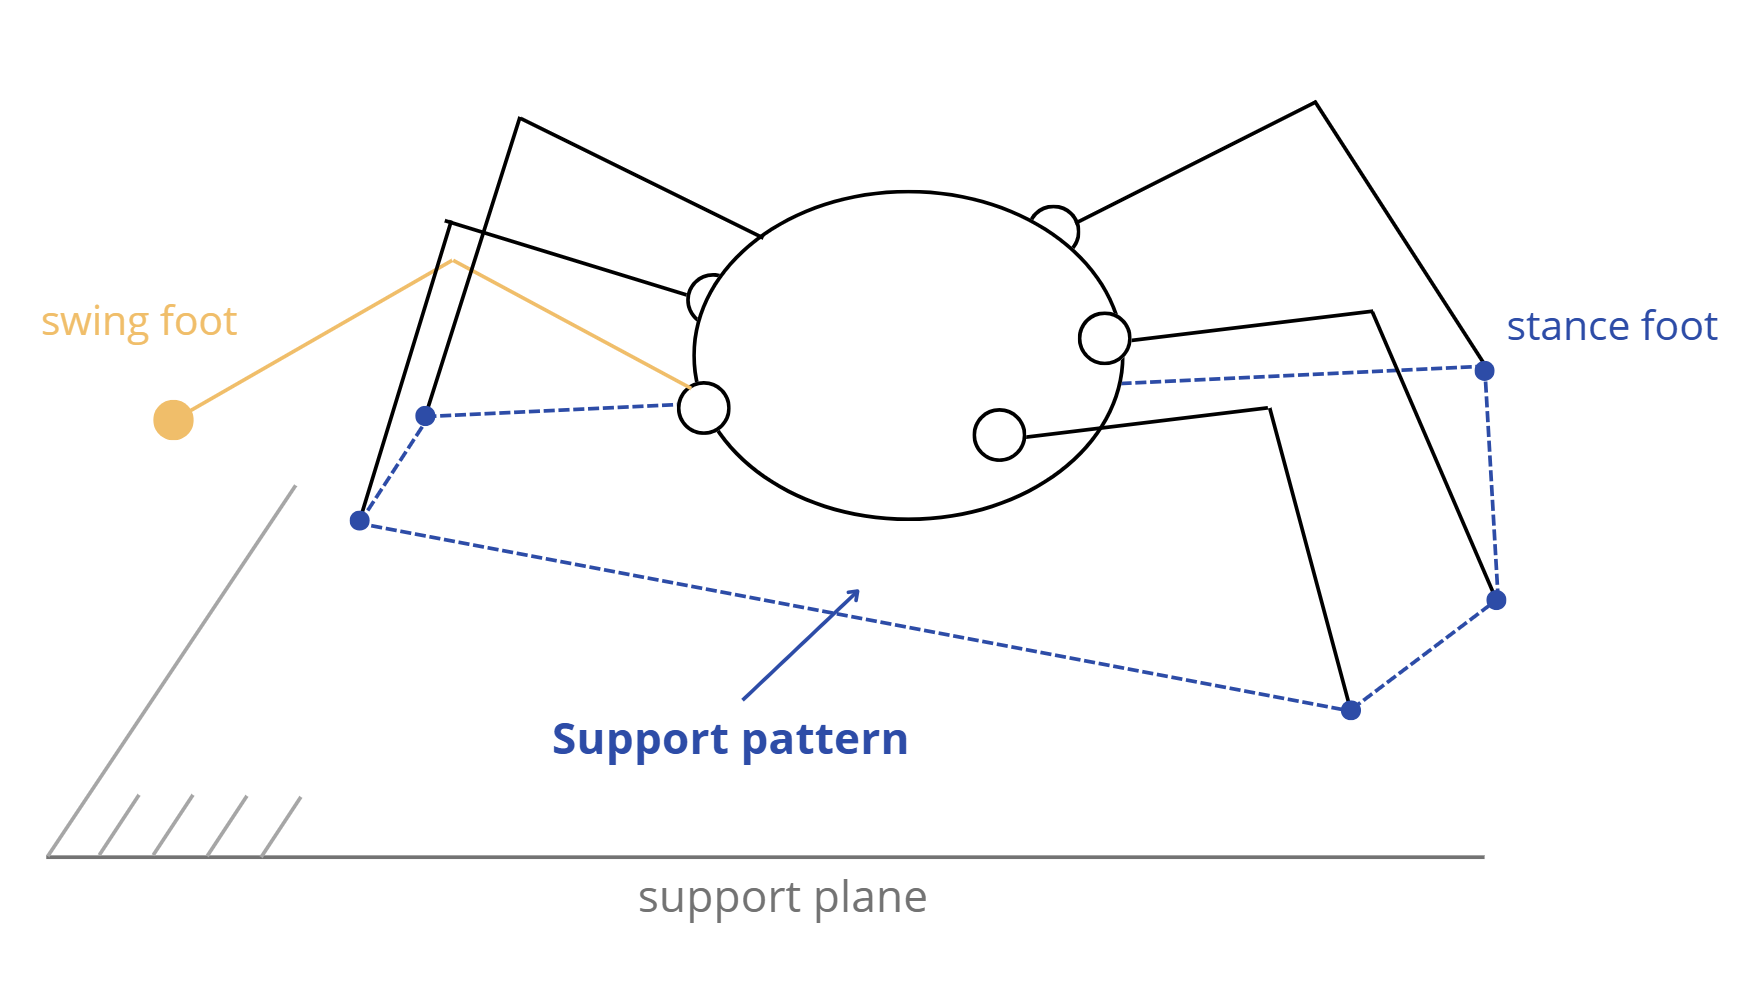
\includegraphics[scale=0.4]{Images/img_ch3/supportpattern1.png}}
    \subfloat{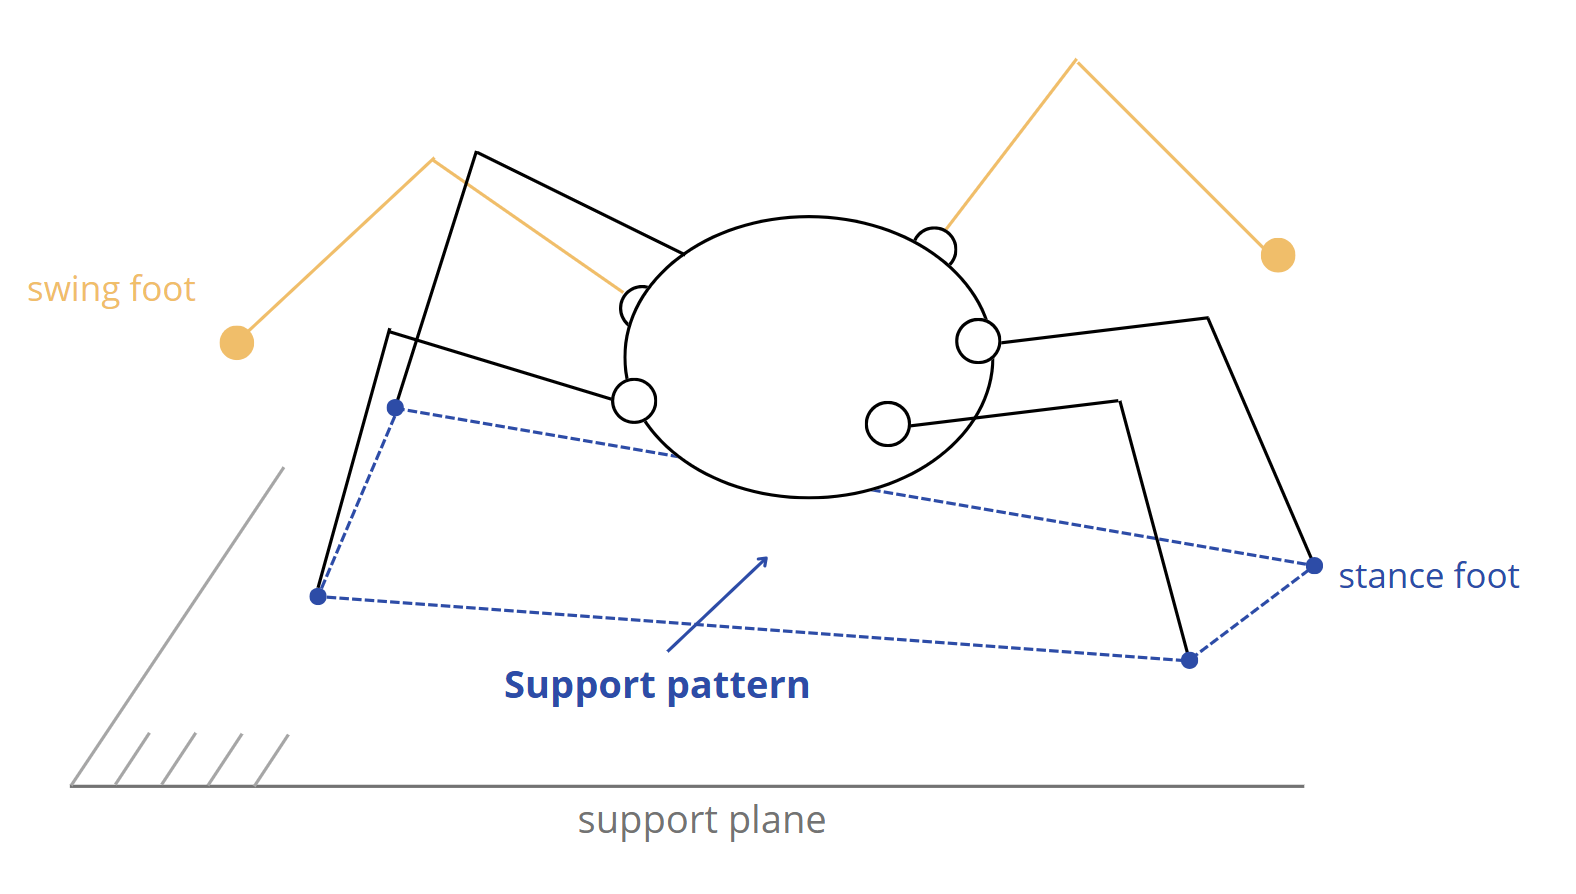
\includegraphics[scale=0.45]{Images/img_ch3/supportpattern2.png}}
    \caption[Examples of support pattern]{Example of support pattern in two different leg configurations.}
    \label{fig:supportPolygon}
\end{figure}

Support patterns are related to the static stability of legged machines, and a theorem to evaluate this stability for a horizontal support plane has been formalized \cite{McGhee}
\begin{definition}\label{def:static_stability}
A legged locomotion machine is \textbf{statically stable} at time $t$ if all legs in contact with the support plane at the given time remain in contact with that plane when all legs of the machine are fixed at their locations at time $t$ and the translational and rotational velocities of the resulting rigid body are simultaneously reduced to zero
\end{definition}
\begin{theorem}\label{th:static_stability}
A legged locomotion machine supported by a stationary horizontal plane surface is \textbf{statically stable} at time $t$ if and only if the vertical projection of the center of gravity of the machine onto the supporting surface lies within its support pattern at the given time
\end{theorem}

Theorem \ref{th:static_stability} holds for an ideal machine not subjected to external disturbances\cite{McGhee}, a notion of relative stability according to this theory is desirable to provide a margin of reliability.


\newpage
\begin{definition}\label{def:static_stability_margin}
\cite{McGhee}The magnitude of the \textbf{static stability margin}(SSM) at time $t$ for an arbitrary support pattern is equal to the shortest distance from the vertical projection of the center of gravity to any point on the boundary of the support pattern. If the pattern is statically stable, the stability margin is positive. Otherwise, it is negative.
\end{definition}

The SSM requires the computation of all the distances of the CoM projection from the support pattern perimeter, McGhee introduced an additional stability margin related to the direction of motion\cite{McGheeRoughLocomotion}:
\begin{definition}\label{def:static_stability_margin}
The magnitude of the \textbf{longitudinal stability margin} (LSM) at time $t$ for an arbitrary support pattern is equal to the shortest distance from the vertical projection of the center of gravity to the front or rear boundary of the support pattern as measured in the direction of travel 
\end{definition}

Using the kinematic model of multi-limbed robots introduced in \ref{sec:forward}, it is possible to reformulate these important concepts mathematically. 
The time dependency is neglected for notation conciseness, but all the quantities described are time-dependent, furthermore, all the 3D vectors above are measured in an inertial frame, for example, the World frame \textbf{w}. 
Remembering that the set of contact limbs has been defined as $J_c$, the support pattern (SP) is given by the convex hull formed by the contact points of the feet in the support plane $\mathbf{P}_{c,j},\forall j \in J_c$:

\begin{equation}
\label{eq:SP}
    SP = \text{Conv}(J_c) = \left\{ \sum_{j \in J_c} \lambda_j \mathbf{P}_{c.j} \;\Bigg|\; \sum_{j \in J_c} \lambda_j = 1, \; \lambda_j \geq 0, \; \forall j \in J_c \right\}
\end{equation}

Denoting with $\mathbf{P}_{CoM}$ the position of the base CoM, with $\mathbf{\overline{P}}_{CoM}$ its vertical projection on the support plane, theorem \ref{th:static_stability} can be reformulated. 
First, it is important to notice that the support plane is assumed horizontal, at height $z_0$ in the inertial frame, so $\mathbf{\overline{P}}_{CoM} = \begin{bmatrix} \overline{x}_{CoM} & \overline{y}_{CoM} & \overline{z}_{CoM}\end{bmatrix}^T \in \mathbb{R}^3$ can be reduced to a 2D vector $\mathbf{\overline{P}}_{CoM} = \begin{bmatrix} \overline{x}_{CoM} & \overline{y}_{CoM}\end{bmatrix}^T$ in the support plane, being $\overline{z}_{CoM} = z_0$ constant.  
This reduction of space allows to formulate the condition of static stability ($\overline{P_{CoM}} \in SP$) using the convex combination condition ($\overline{\mathbf{P}}_{CoM}$ is given by a convex combination of SP vertex, with the same formulation of SP points):
\begin{theorem}\label{th:static_stability_math}
A legged locomotion machine supported by a stationary horizontal plane surface is \textbf{statically stable} at time $t$ if and only if \\ $\exists \lambda_j \ge 0 \;,\; j\in J_c \;|\; \sum_{j \in J_c} \lambda_j = 1 \;, \overline{\mathbf{P}}_{CoM} = \sum_{j \in J_c} \lambda_j \mathbf{P}_{c.j}$
\end{theorem}

\newpage
Furthermore, with the same logic, it is possible to define a function $\sigma_{SS}(\overline{\mathbf{P}}_{CoM})$ equal to $+1$ if ($\overline{\mathbf{P}_{CoM}} \in SP$), $-1$ otherwise, this is needed to define the SSM correctly. 

\begin{equation}
\label{eq:sigma_SS}
\sigma_{SS}(\overline{\mathbf{P}}_{CoM}) = \
    \begin{cases}
    +1 \quad\text{ if } \exists \lambda_j \ge 0 \;,\; j\in J_c \;|\; \sum_{j \in J_c} \lambda_j = 1 \;, \overline{\mathbf{P}}_{CoM} = \sum_{j \in J_c} \lambda_j \mathbf{P}_{c.j}\\ \\ 
    -1 \quad\text{ otherwise}
    \end{cases}
\end{equation}

Finally, denoting with $\partial SP$ the perimeter of the SP, identified by all the edges $\overline{\mathbf{P}_{c.j}\mathbf{P}_{c.j+1}}\;,\; \forall j\in J_c$, the SSM can be defined as:
\begin{equation}
\label{eq:SSM_1}
    SSM = \sigma_{SS}(\overline{\mathbf{P}}_{CoM}) \cdot\min_{\mathbf{P}\in\partial SP}{\text{dist}(\overline{\mathbf{P}}_{CoM}, \mathbf{P})}
\end{equation}
Where dist($\mathbf{P_1}$,$\mathbf{P_2}$) denotes a measure of distance between $\mathbf{P_1}$ and $\mathbf{P_2}$, for example, the Euclidean distance in 3D space  $||\mathbf{P_2} - \mathbf{P_1}||$. 
This can be further reformulated considering that the SP perimeter is composed by the segments connecting the sequence of contact points: 
\begin{equation}
\label{eq:SSM_2}
    SSM =\sigma_{SS}(\overline{\mathbf{P}}_{CoM})\cdot \min_{j}{\frac{\left|(\mathbf{P}_{c,j+1} - \mathbf{P}_{c,j})  \times (\mathbf{P}_{c,j} - \mathbf{\overline{P}}_{CoM})\right|}{||\mathbf{P}_{c,j+1} - \mathbf{P}_{c,j}||}}
\end{equation}

Multiplying by $\sigma_{SS}(\overline{\mathbf{P}}_{CoM})$ is important to maintain the characteristic of the SSM to be positive is the legged robot is stable, negative otherwise. Clearly, the bigger the SSM and higher the level of stability, $SSM=0$ is a critical boundary condition, when $SSM < 0$ the robot is unstable.

To define the LSM, if the direction of motion is identified by the translational base velocity vector $\dot{\mathbf{p}}_b$, a mathematical formulation of that index requires also the identification of the intersection between the projection of the direction of motion in the support plane $\overline{\dot{\mathbf{p}}}_b$ and the support polygon perimeter $\partial SP$. This is not addressed here, instead Figure\ref{fig:SP_SSM_LSM} is a graphical representation of this, including the SP and the SSM.

\begin{figure}[H]
    \centering
    \subfloat[Stable configuration.\label{fig:stableLegged}]{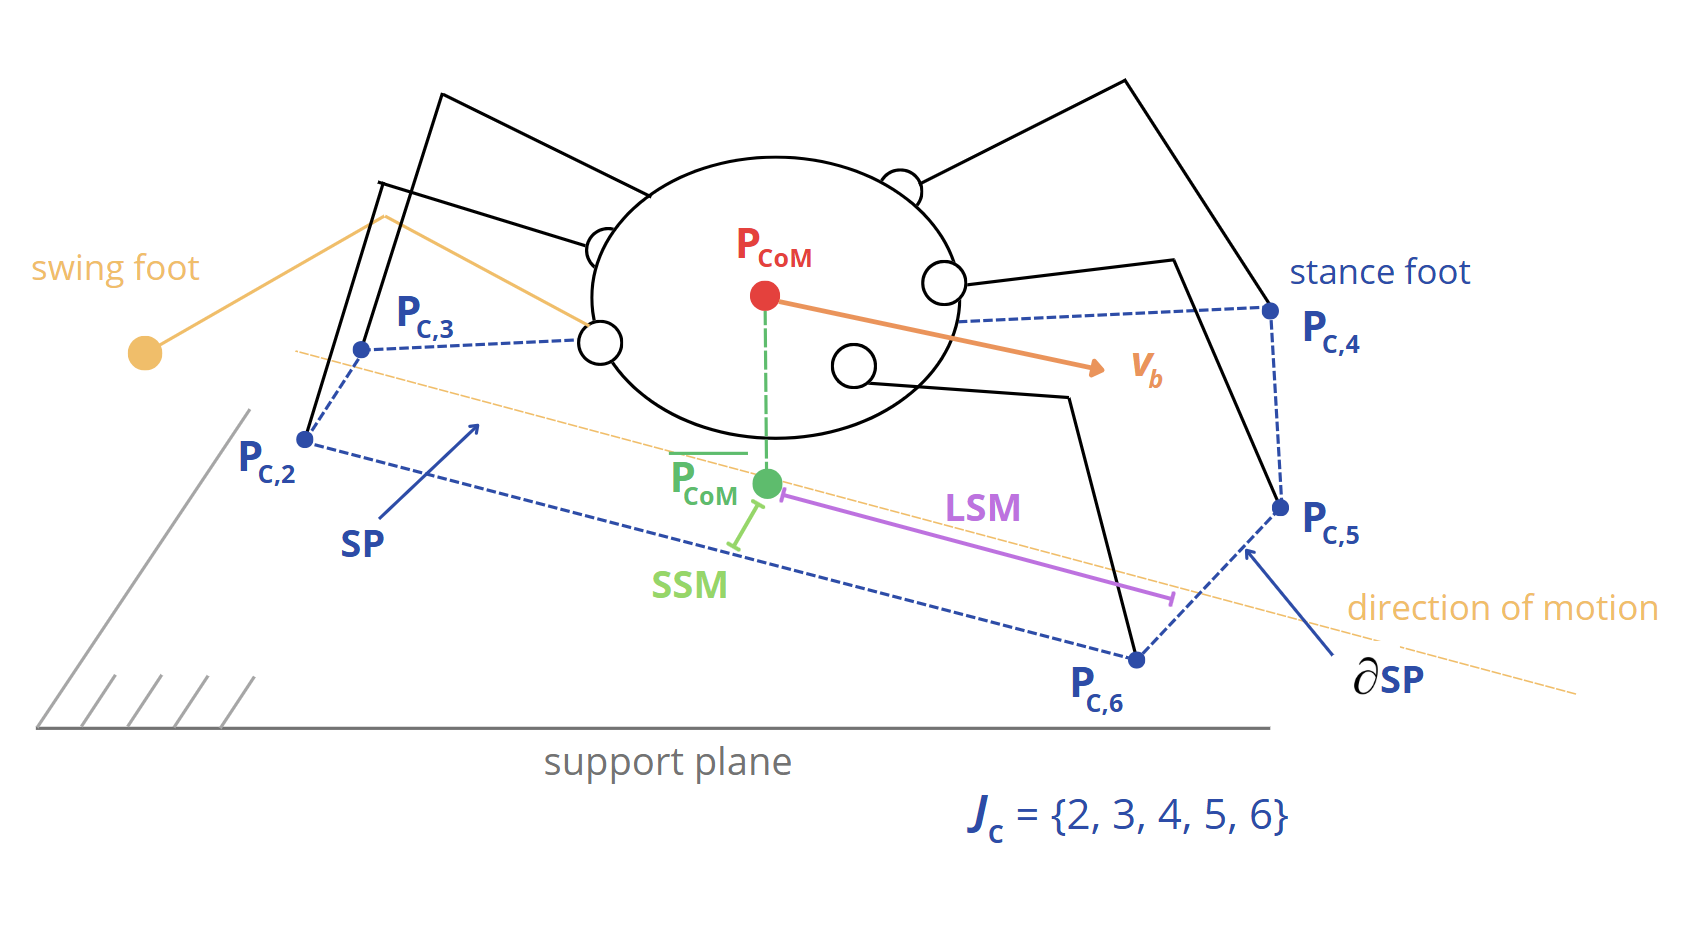
\includegraphics[scale=0.45]{Images/img_ch3/StabilityMargin1.png}}
    \subfloat[Unstable configuration.\label{fig:unstableLegged}]{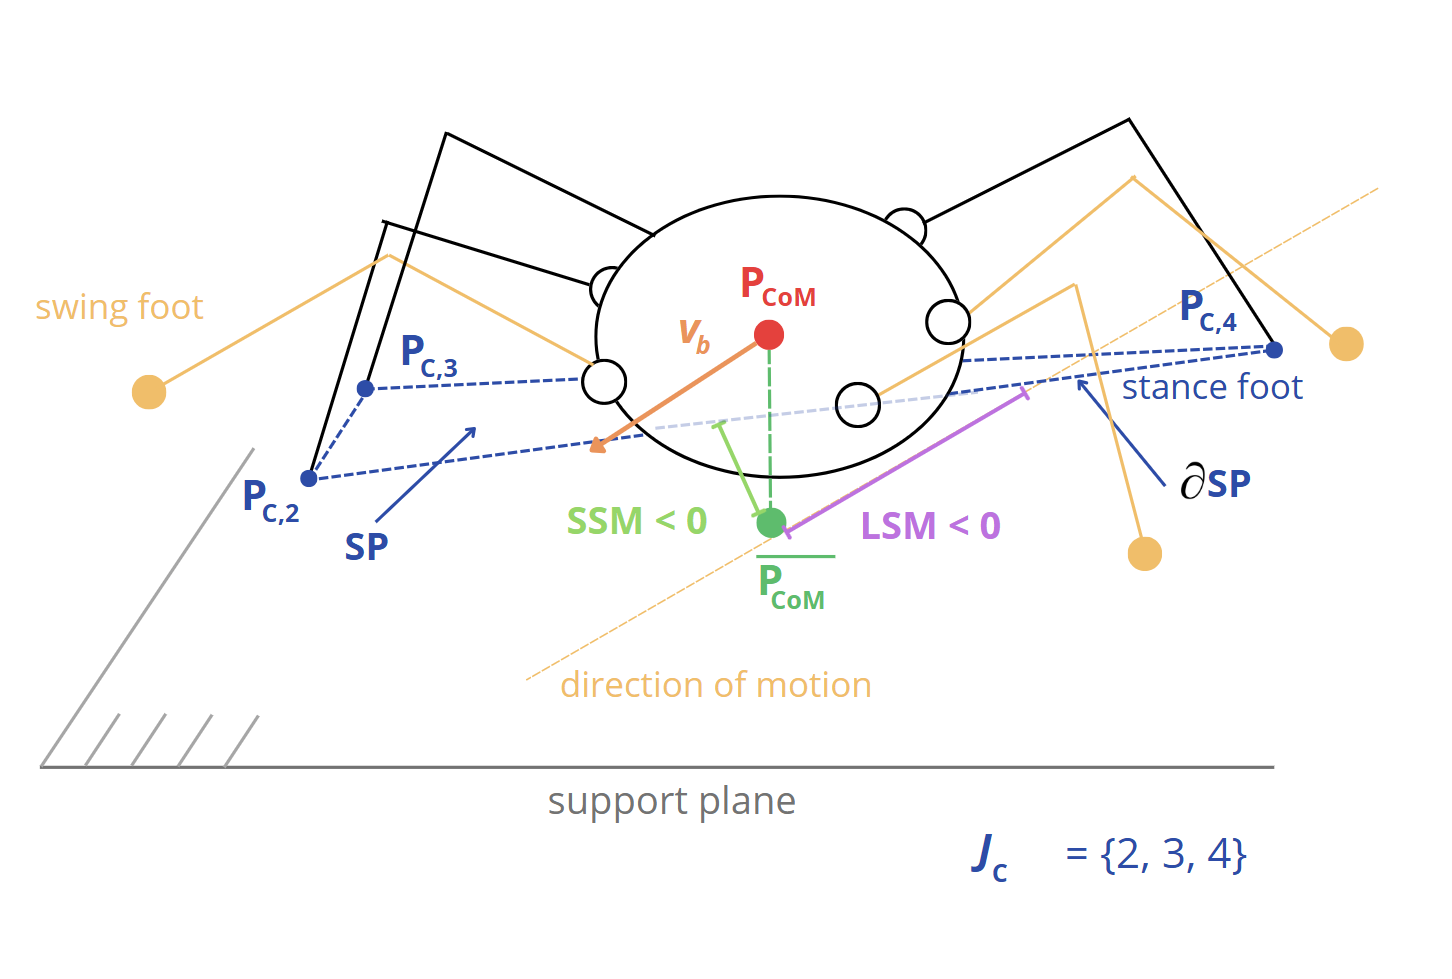
\includegraphics[scale=0.45]{Images/img_ch3/StabilityMargin2.png}}
    \caption[Examples of stability evaluation]{Example of statically stable and unstable robot configuration.}
    \label{fig:SP_SSM_LSM}
\end{figure}

As discussed in the previous chapter during the kinematic modeling of limbed robots, the base pose depends on all leg configuration $\mathbf{q} \in \mathbb{R}^n$, then $\mathbf{P}_{CoM}(\mathbf{q})$. This dependency is neglected in the notation, but it is important to remember that the robot is in a statically stable or unstable configuration depending on the leg joint state. 

This stability criteria, formalized from Equation \ref{eq:SP} to \ref{eq:SSM_2}, depends only on geometrical analysis and simple contact assumptions, and the validity is restricted when the support plane is horizontal (or at least approximately flat). Even if flat terrains of operation have been assumed for this research, it is relevant to give a brief overview of other methods that account for robot dynamics and interaction forces. 

\subsection{Dynamic Stability}
\label{sec:dynamic_stability}

One of the first studies on dynamic stability comes from the work of Vukobratović on anthropomorphic systems\cite{ZMP_vukobratovic}, which led to the definition of the zero moment point (ZMP). The ZMP is the point where the net moment of inertia force and gravity on the ground has no component in the horizontal direction\cite{ZMP_Vukobratovic_2}, and stability is maintained when it lays inside the SP. It has been widely used to evaluate both bipedal and multi-legged robot stability and gait generation \cite{ZMP_bipedal}\cite{ZMP_quadruped}\cite{ZMP_quadruped2}\cite{HandbookLegged}. It can be proven that when quasi-static motion is involved, ZMP and SSM stability criteria are equivalent\cite{HandbookLegged}.

Both the SSM and ZMP measure a stability margin as the distance of a point from the SP borders, the SP is a planar surface by definition. The limitation of the SSM is that that plane must be almost horizontal, while the ZMP, which considers gravity and inertial effect, is reliable also for slopes. In both cases, a limitation is clear: a plane where all leg contact points lay has to be identified, and this is not always possible, as represented in Fig.\ref{fig:rough_terrain}.
For this reason, the equilibrium of robots walking in rough terrain cannot be evaluated with those classical methods.

\begin{figure}[H]
    \centering
    \subfloat{
        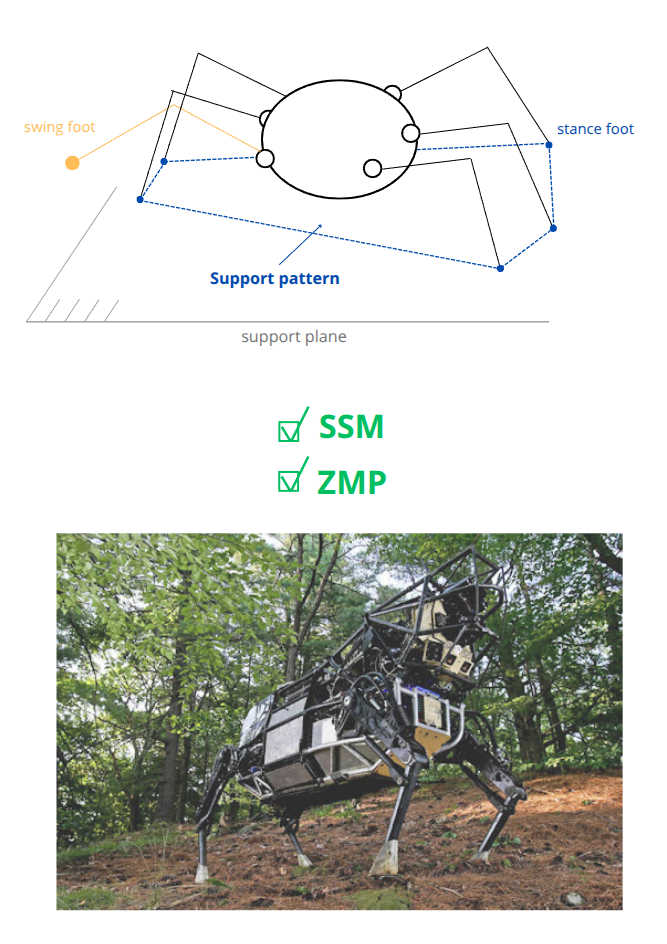
\includegraphics[scale=0.2]{Images/img_ch3/roughterrain1.png}
    }
    \subfloat{
        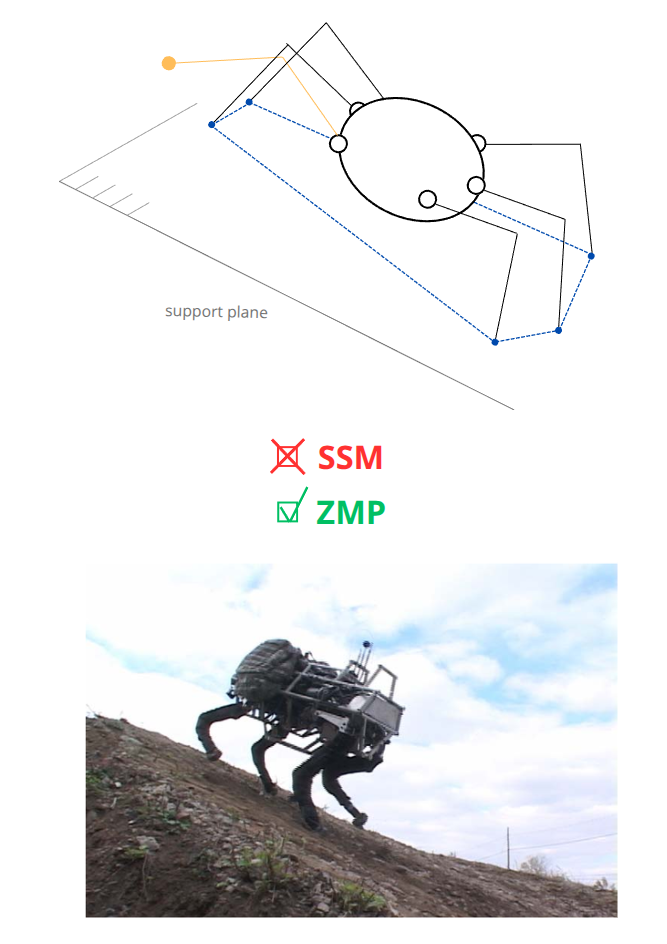
\includegraphics[scale=0.2]{Images/img_ch3/roughterrain2.png}
    }
    \subfloat{
        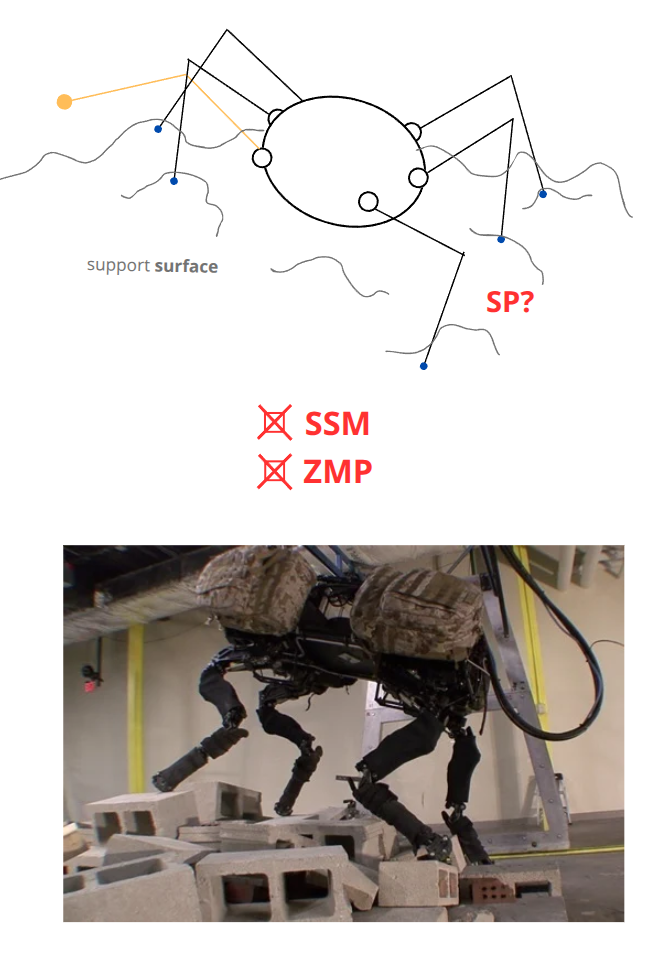
\includegraphics[scale=0.2]{Images/img_ch3/roughterrain3.png}
    }
    \caption[Overview of SSM and SMP usage]{Schematic representation of cases where SSM and ZMP can be used, with real-life examples based on Boston Dynamics Big Dog\cite{BigDogRoughTerrain}}
    \label{fig:rough_terrain}
\end{figure}


 S.Hirose, another pioneer of legged robotics, defined the tumble stability (TS) as a dynamic equilibrium criterion\cite{TumbleStability}. Identifying the tumbling axis as the line connecting two different contact points ($\overline{\mathbf{P}_{c,j}\mathbf{P}_{c,k}} \;, \; j,k \in J_c\ ;,\; j \not= k$), and the tumbling moment $\mathbf{M}_{j,k}$ as the total moment around the tumbling axis, computed from the effect of gravitational, inertial and external forces\cite{Ribeiro2023reaction}\cite{KentaroUnoPhD}.
 Under no slipping condition, the equilibrium is ensured when tipping over is counteracted by another contact foot. 
 Details on the computation of $\mathbf{M}_{j,k}$ and the stability constrain formulation are out of this scope, the resultant stability margin coming from this analysis is the tumble stability margin: 
\begin{equation}
\label{eq:TSM}
    TSM =\min_{j,k \in J_c}{\frac{\mathbf{M}_{j,k}}{mg}}
\end{equation}
where $m$ denotes the total mass of the robot. 

The tumble stability concept has been extended by W.Ribeiro for applications in microgravity, introducing the concepts of gravito inertia acceleration (GIA) and stability polyhedron\cite{GIA_polyedron}\cite{Ribeiro2023reaction}. 
The GIA is a vector derived from the combination of the robot's inertial acceleration and the gravity vector, while the support polyhedron is a 3D region defined from tumble stability constraints.
While the previously introduced support pattern is a 2D region, and the stability is evaluated with the ZMP or CoM projection, the GIA vector, introduces an additional dimension, and stability is guaranteed when the GIA vector is contained in the support polyhedron (as represented in Fig.\ref{fig:GIA}).

\begin{figure}[H]
    \centering
    \subfloat[Stable limit plane .\label{fig:stableregion}]{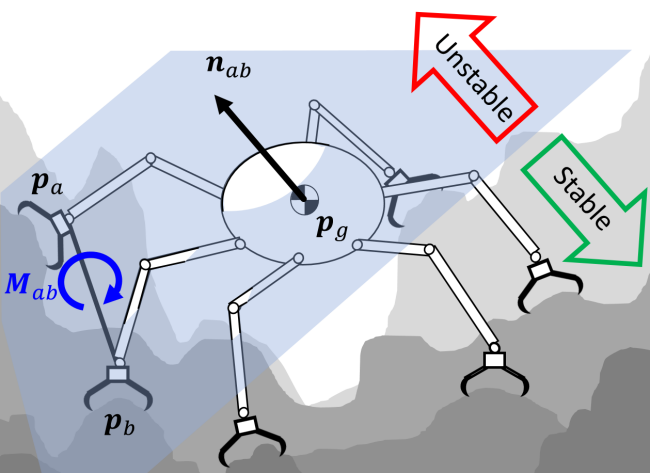
\includegraphics[scale=0.3]{Images/img_ch3/GIA1.png}}
    \subfloat[Stability polyhedron and GIA vector\label{fig:gia_polyhedron}]{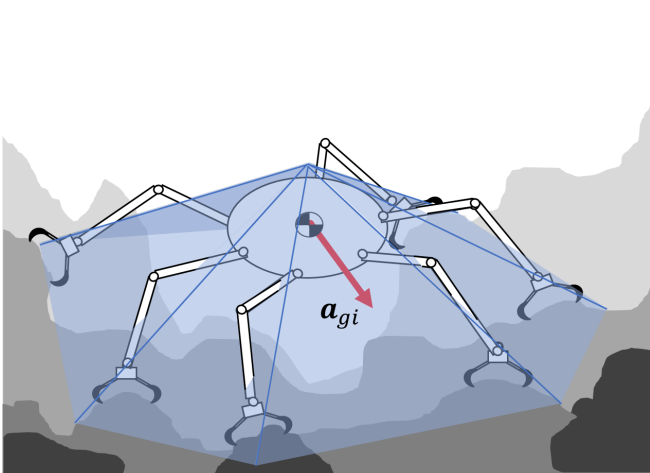
\includegraphics[scale=0.3]{Images/img_ch3/GIA2.png}}
    \caption[Schematic representation of GIA and support polyhedron]{\cite{GIA_polyedron}\cite{Ribeiro2023reaction} representation of GIA and support polyhedron configuration.}
    \label{fig:GIA}
\end{figure}



Both the TS and GIA can be formulated with gripping forces, making those methods suitable for climbing robots\cite{Ribeiro2019climbing}\cite{RibeiroGroundGripping}. 

The state of the art on stability analysis for legged robots is vast, in the next, additional criteria based on energetic considerations are described. 

\subsection{Energetic Stability}
\label{sec:gripping_stability}

For rough terrain, Messuri and Klein introduce an energy base criterion, the \textbf{energy stability margin} (ESM)\cite{ESM}, quantifying the minimum potential energy required to tumble the robot around the edge of the support polygon (a subset of the tumble axis, $\overline{\mathbf{P}_{c.k}\mathbf{P}_{c.k+1}}$ ):
\begin{equation}
\label{eq:ESM}
    ESM =\min_{k\in J_c}{mgh_k}
\end{equation}
In this formula, $h_k$ is the CoM height variation during the tumble, M is the total mass of the robot, and g is the gravitational acceleration. 

This index has been redefined  as \textbf{Normlaized Energy Stability Margin} (NESM) by Hirose, considering only the variation of the robot's CoM height \cite{NormalizedEnergySM}

\begin{equation}
\label{eq:NESM}
    NESM = \frac{ESM}{mg} = \min_{k \in J_c}{h_k}
\end{equation}

Both the ESM and NESM are efficient measures to evaluate statically stable walking on rough and sloped terrains\cite{EnergyIndexhexapod}, but when relevant dynamic effects influence motion (as fast locomotion or manipulation), these indices are not reliable. 
position
From the idea of Ghasempoor and Sepehri\cite{DESMidea} to measure wheel-based mobile manipulator stability, Garcia \cite{GarciaDESM} extend it for walking machines. 
The ESM has been extended, including the presence of other dynamical effects, like inertial forces or manipulation effects, computing the increase of mechanical energy that the CoM experiences during the tumble. 
The resulting \textbf{Normalized Dynamics Energy Stability Margin} (NDESM) is defined as the smallest of the stability levels required to tumble the robot around the support
polygon, normalized to the robot mass: 
\begin{equation}
\label{eq:NDESM}
    NDESM = \min_{k \in J_c}{\frac{E_k}{mg}}
\end{equation}
where $E_k$ identify the stability level of the $k^{th}$ edge of the support polygon,
which physically means the increment of mechanical energy required to tumble
the robot around that edge. 

In his extensive studies on the SILO 4 robot\cite{QuadrupedLocomotion}, Garcia introduce new approaches to the stability analysis, introducing new stability margins related to actuator limitation, such as: 
\begin{itemize}
    \setlength\itemsep{-0.7em} 
    \item \textbf{ torque limit stability margin}: related to the motor torque usage respect the limits
     \item \textbf{ current stability margin} related to the electric current usage respect the limits
\end{itemize}
Furthermore, normalized quantities and a global static-stability vector have been defined to analyze realistic constrained static stability, but the description of it is not relevant here.

\section{Performance Indices}
\label{sec:dynamic_indices}

The measures and criteria discussed until now address the evaluation of stability from geometrical, dynamic, and energetic considerations, but insights into system consumption efficiency and locomotion performance are not investigated. 

\subsection{Energetic Efficiency}
\label{sec:energetic_efficecny}

A possible energetic performance measure was proposed for a monopod robot\cite{SpecificResistance2}, based on the specific resistance $\varepsilon$ by Gabrielli and Von Karamn\cite{SpecificResistance1}, which considers not only the output power but also the mass moved and the obtained velocity. 
If $P$ denotes the output power, $m$ the total mass of the system, and $v_{max}$ the maximum speed of transportation, this quantity is defined as 
\begin{equation}
\label{eq:NESM}
    \varepsilon = \frac{P}{mgv_{max}}  
\end{equation}

This quantity can be evaluated in function of the locomotion  velocity as: 
\begin{equation}
\label{eq:NESM_2}
    \varepsilon(v) = \frac{P(v)}{mgv}  
\end{equation}
This can be used to compare different robots regardless of size, speed, or configuration.
An alternative way to compute this measure, comes from the definition of Gabrielli and von Karman\cite{SpecificResistance1}: 
\begin{equation}
\label{eq:NESM_2}
    \varepsilon = \frac{E}{mgd}  
\end{equation}
where $E$ is the total energy consumption for a travel of
distance $d$, $m$ is the total mass of the vehicle, and $g$ is
the acceleration due to gravity\cite{HandbookLegged}.

With a similar approach, energy consumption has been analyzed for a realistic six-legged robot\cite{EnergyIndexhexapod}, using the average locomotion power $P_{av}$ and the average velocity $v_{av}$ with the same formula as in Eq.\ref{eq:NESM_2}, denoting it as \textbf{specific energy consumption}.  
This same index has also been referred to as \textbf{cost of Transportation}(CoT)\cite{CosOfTransport} because it is a metric of the energetic economy of locomotion. 

Other interesting power efficiency indices have been introduced by M.F.Silva\cite{LocomotionPerformance}, such as the mean absolute power, mean power dispersion, and mean power lost, based on different power analyses on limb motors during locomotion.

\subsection{Mobility Efficiency}
\label{sec:mobility_efficecny}

When planning motion tasks for a limbed robot, stability, and efficiency should be taken into account, but dexterity and maneuverability are also important. 
For example, under the assumption of quasi-static motion in a horizontal plane, the SP criterion is used to evaluate stability, and according to the SSM, the optimal configuration (where the SSM is maximized) corresponds always to the one where the CoM project in the center of the SP. This requirement can lead to limb configurations close to singularities and joint limits(as represented in Fig.\ref{fig:bad_config}), degrading the dexterity of the system for any future motion.

\begin{figure}[H]
    \centering
    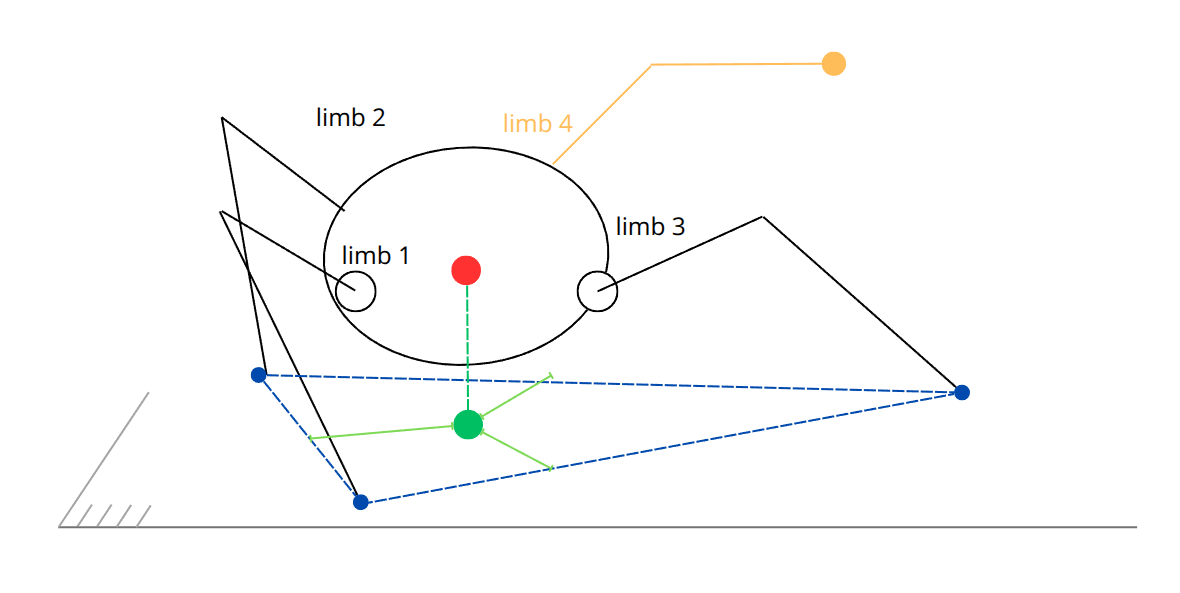
\includegraphics[width=0.7\textwidth]{Images/img_ch3/BadConfig.png}
    \caption{Example of undesired limbed robot configuration with optimal SSM}
    \label{fig:bad_config}
\end{figure}

The literature lacks a measure of ease of motion in a given configuration for multi-limbed robots, which could be relevant when planning complex multipurpose tasks.
In this section, the existing tools and research on limbed robot locomotion performances are summarized, in the next, a new measure to generalize and quantify manipulability for limbed robots is defined and discussed. 

F.Silva\cite{LocomotionPerformance} defined a \textbf{Locomobility Measure} from the concept of arm manipulability\cite{ManipulabilityYoshikawa}, applied to the limb during motion. 
With the same notation of chapter \ref{sec:differential}, the Jacobian matrix relating the limb root with the foot end is $\mathbf{J}_j(\mathbf{q}_j)$, with $\mathbf{J_P}_j(\mathbf{q}_j)$ denoting the translational part, then the translational velocity manipulability ellipsoid is described by the $3\times3$ positive definite matrix $\mathbf{J_P}_j(\mathbf{q}_j)\mathbf{J^T_P}_j(\mathbf{q}_j)$. 
Then, the locomobility index over a gait cycle $T$ is computed as: 
\begin{equation}
\label{eq:Locomobility}
    L_F = \frac{1}{T} \int_0^T{E_F(t)dt}  
\end{equation}
Where $E_F$ denotes the distance between the center of the foot translational ellipsoid and its intersection with the tangent to the desired foot trajectory. 
The best foot trajectory is the one that maximizes $L_F$. 
This index is useful to optimize the ease of foot motion along the trajectory during walking.

Another measure of the system locomotion capability is the workspace (def.\ref{def:workspace} in the previous chapter), which can be mapped from the limb tip to the reachable base positions, considering closed kinematic chain constraints in the contact points (with parallel manipulator model). This is a measure often used in the design phase for robot limbs, but rarely used in the base position space \cite{HexapodBaseWorkspace}\cite{HexapodBaseWorkspace2}. In free space, the limb workspace depends just on its mechanical design and joint limits, and after the limb development, it is fixed. The base workspace instead depends both on the contact limb workspace and contact points, which can be useful during foothold planning along the planned path \cite{LIMBEROTakadaThesis}\cite{LeggedPlanning1}\cite{threeLeggedDexterity}
. 

None of the measures described above provide an intuitive way to define optimal configuration in terms of base manipulability and dexterity. The only works with similar desired performance metrics are "general multi limb robots analysis" by C.Melchiorri \textit{et all} \cite{MultiLimbManipulabilityMelchiorri} and "velocity workspace analysis for multi-legged robots" by J.Lee \textit{et all}  
\cite{velocityWorkspacePolytope}.
In \cite{MultiLimbManipulabilityMelchiorri}, mobility, kinematic, and manipulability of multiple limb robots cooperating to move an object are analyzed. To define a generic framework for various similar systems (such as dexterous hands (multi-fingers interaction) and legged vehicles), the assumptions made on cooperation are very general.
This generality is both its strength and its limitation, it is complex to define, and not many examples of its usage can be found in literature.  

In \cite{velocityWorkspacePolytope} instead, walking robot velocity manipulability is analyzed with an approach similar to this research contribution, using the cooperative manipulators' parallelism introduced in section \ref{sec:leggedLimbedDK}. "Hard-foot" ground interaction is considered, constraining any moment to zero. With this model, the analysis has been conducted only for manipulability of translational base motion, represented through polytope\cite{PolytopesManipulability}. 


\section{Novel Base Manipulability Index}
\label{sec:base_manipolability}

As introduced in the previous section, the literature lacks tools to analyze online and intuitively the rotational and translational maneuverability of limbed robot configuration.
The only works trying to implement something similar are \cite{DualArmTaskManipulability} \cite{MultiLimbManipulabilityMelchiorri} for cooperative manipulators, and \cite{velocityWorkspacePolytope} for limbed robots. 
These works are 25 years old and applications based on these ideas cannot be found in literature.

Despite this, a measure of manipulability is very useful to define optimal task-consistent robot configuration, especially for multi-limb robots, where manipulation capabilities are intrinsic in limbs design.

To develop this theory, the manipulability ellipsoid (ME) is an intuitive and powerful geometrical entity to understand the capabilities of a robotic arm\cite{ManipulabilityYoshikawa}, and some researchers tried to adapt the theory for humanoid robots
\cite{BipedEllipsoid1}\cite{BipedEllipsoid2}\cite{BipedEllipsoid3}\cite{BipedEllipsoid4}\cite{BipedEllipsoid5}. This thesis contribution aims to break years of silence in research on manipulability theory for multi-limbed machines by showing the possibilities it can open up. Moreover, the need for this tool arose from the main problem addressed in this thesis, in fact it is used in chapter \ref{ch:chapter_five} to define properly an efficient adaptable motion sequence. 


Here, the \textbf{base ME} is introduced as an extension of the extensively used manipulators' ME theory, taking inspiration from the work of Professor B.Siciliano on space manipulability ellipsoids for multiple-arm systems\cite{MultiArmManipulability}\cite{DualArmManipulability}. Differently from \cite{MultiLimbManipulabilityMelchiorri} and \cite{velocityWorkspacePolytope}, his model is elegant, intuitive, and simple to use online, opening new possibilities for optimal motion adaptation at runtime, based on manipulability index maximization. 

% Both T.Yoshikawa's theory\cite{ManipulabilityYoshikawa}
% \cite{YoshikawaRedundancy}\cite{YoshikawaRoboticsBook}\cite{TRManipulability} of ME for single manipulators and B.siciliano's one \cite{DualArmManipulability}
% \cite{MultiArmManipulability} for cooperative manipulators are explained in Appendix \ref{ch:appendixB}


\subsection{Multi-limb Robot Base Manipulability Ellipsoid}
\label{sec:multi_limb_coopmanipulators}

In this section, the hypothesis and the intuitions behind this modeling approach are introduced, and then the kinetostatic and differential kinematic model considered is reported. Finally, the extension of multiarm ME to multi-limb robot base manipulability ellipsoid (BME) is defined.

\subsubsection{Assumptions and Duality}
\label{sec:multi_limb_coopmanipulators}

The multi-limbed robot-multiarm duality is inspired by the similar behavior between the two systems (as schematically represented in Fig.\ref{fig:MultiArmLimbed}), and it is possible when the assumptions listed below hold.

As multiple arms with fixed bases cooperate to move an object in space, a multi-limb robot with fixed contacts reconfigures the limbs to move the torso. 
This behavior is based on the hypothesis of \textbf{contact limb motion propagation without penetration} (\textit{Assumption 1}), as introduced in section \ref{sec:leggedLimbedIK}, and represented intuitively in Fig.\ref{fig:BaseMotionIK}. 
From this, the similarity between the base of each manipulator and the corresponding limb contact point is clear.

Furthermore, tight grasp and rigid object\cite{MultiArmManipulability} is considered for the multiarm system (\textit{Assumption 2}), likewise, the limb root is mechanically attached to the robot torso. 

A schematic view of this is represented in Fig.\ref{fig:MultilimbMultiArm} below. 

\begin{figure}[H]
    \centering
    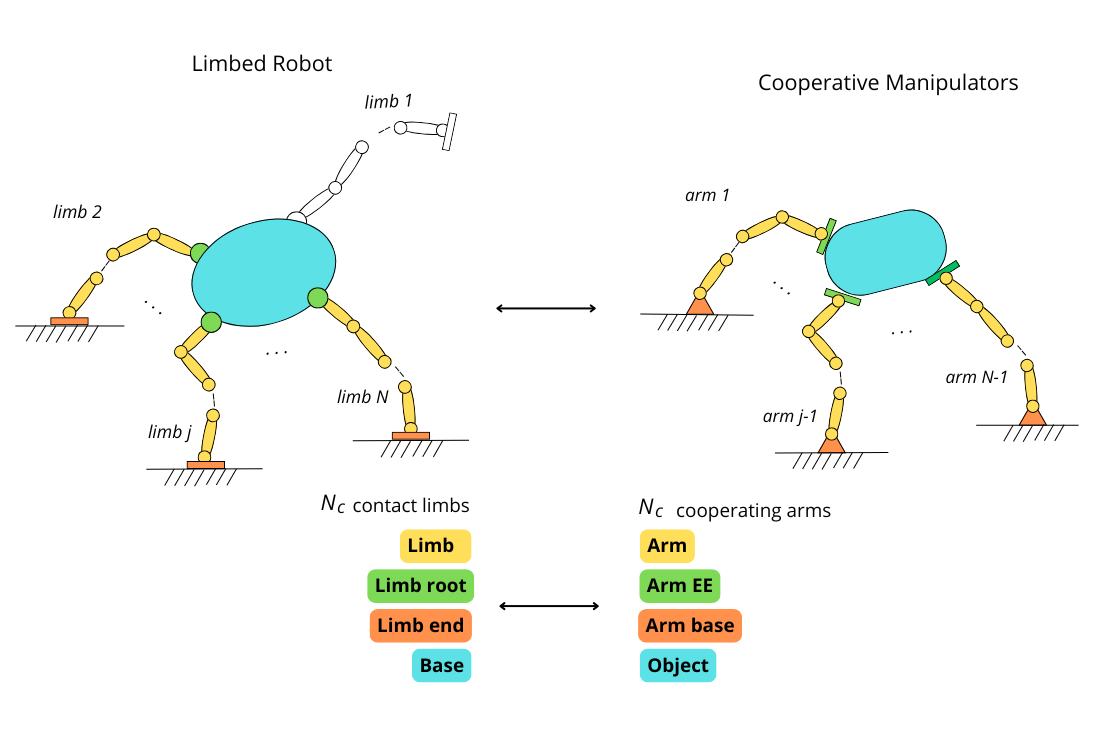
\includegraphics[width=0.9\textwidth]{Images/img_ch3/MultilimbMultiArm.png}
    \caption{Schematic representation of multi-limbed robots and cooperative arms duality}
    \label{fig:MultilimbMultiArm}
\end{figure}

\subsubsection{Kinematic Model for Multi-Limb Robot Base and BME}
\label{sec:multi_limb_coopmanipulators}

The derivation of the kinetostatic model for a multiarm system\cite{MultiArmManipulability} and the quantities involved are defined in \cite{MultiArmManipulability}, here the relevant quantities and equations are summarized for a multi-limb robot. All the vectors are measured in the base frame and represented in Fig.\ref{fig:multilimbmodel}.

\begin{figure}[H]
    \centering
    \subfloat[Frame references and DOFs.\label{fig:multilimbdof}]{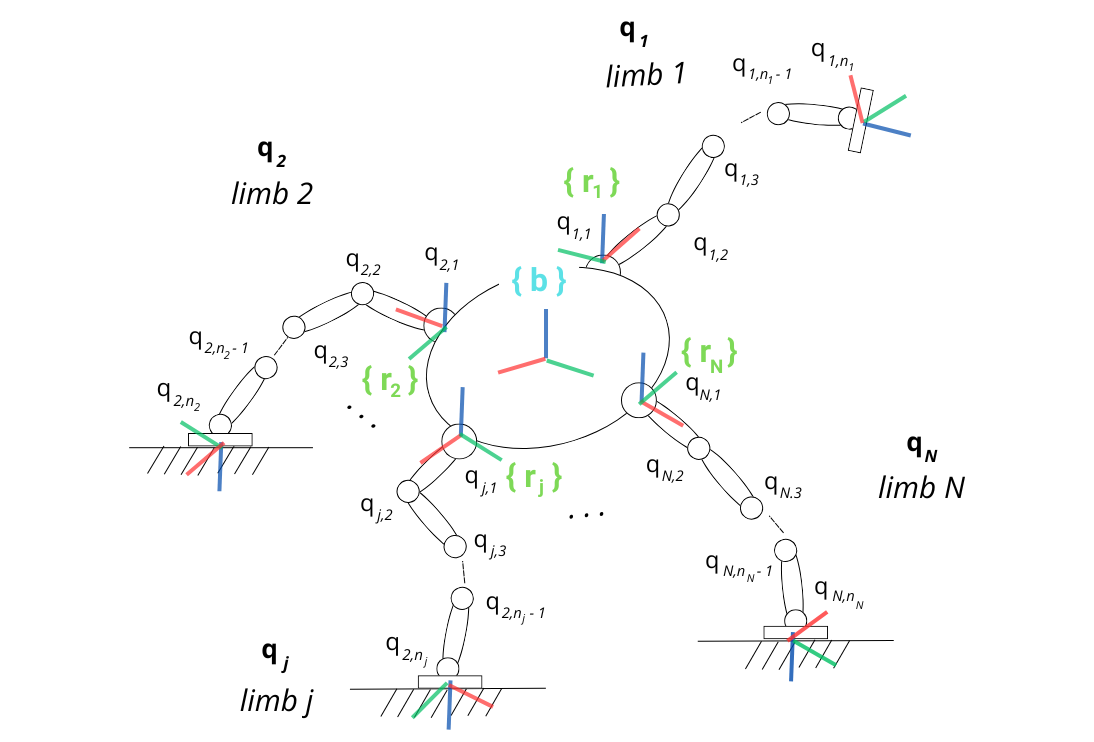
\includegraphics[width=0.8\textwidth]{Images/img_ch3/multilimbmodelDOF.png}}\\
    \subfloat[Relevant vectors.\label{fig:miultilimbvec}]{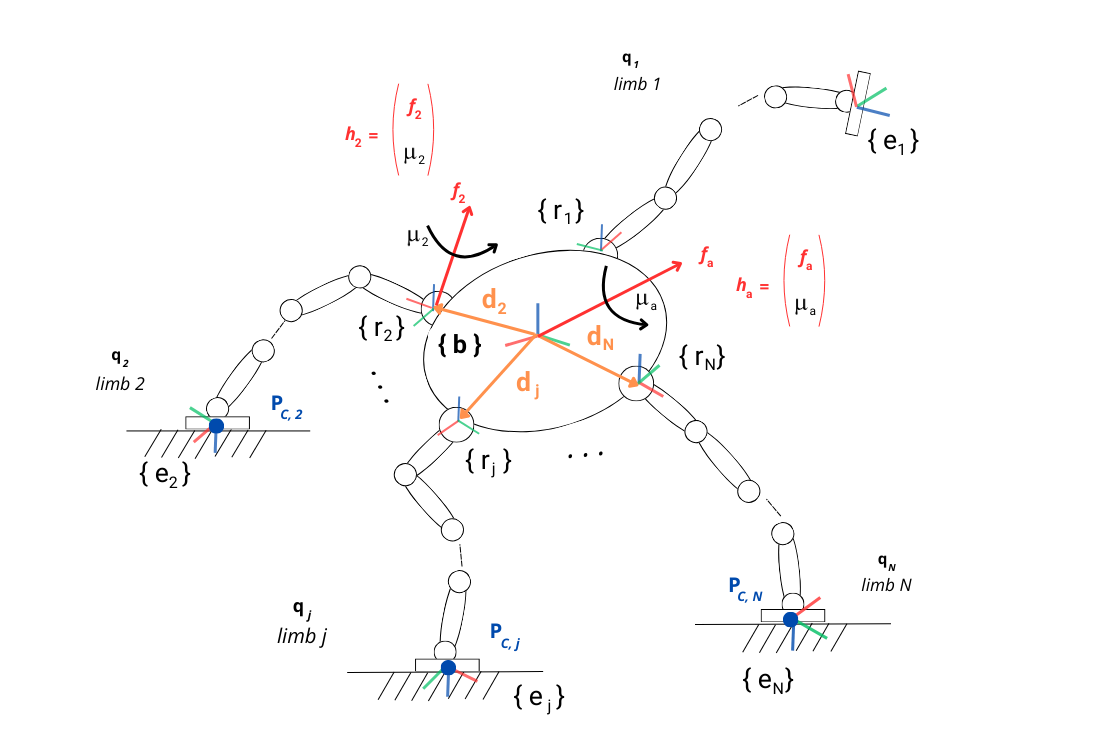
\includegraphics[width=0.8\textwidth]{Images/img_ch3/multilimbmodelVector.png}} 
    \caption[Multi-limb robots frames and vectors]{Relevant frames, DOFs and vector in multi-limb robots}
    \label{fig:multilimbmodel}
\end{figure}

\begin{figure}[H]
    \centering
    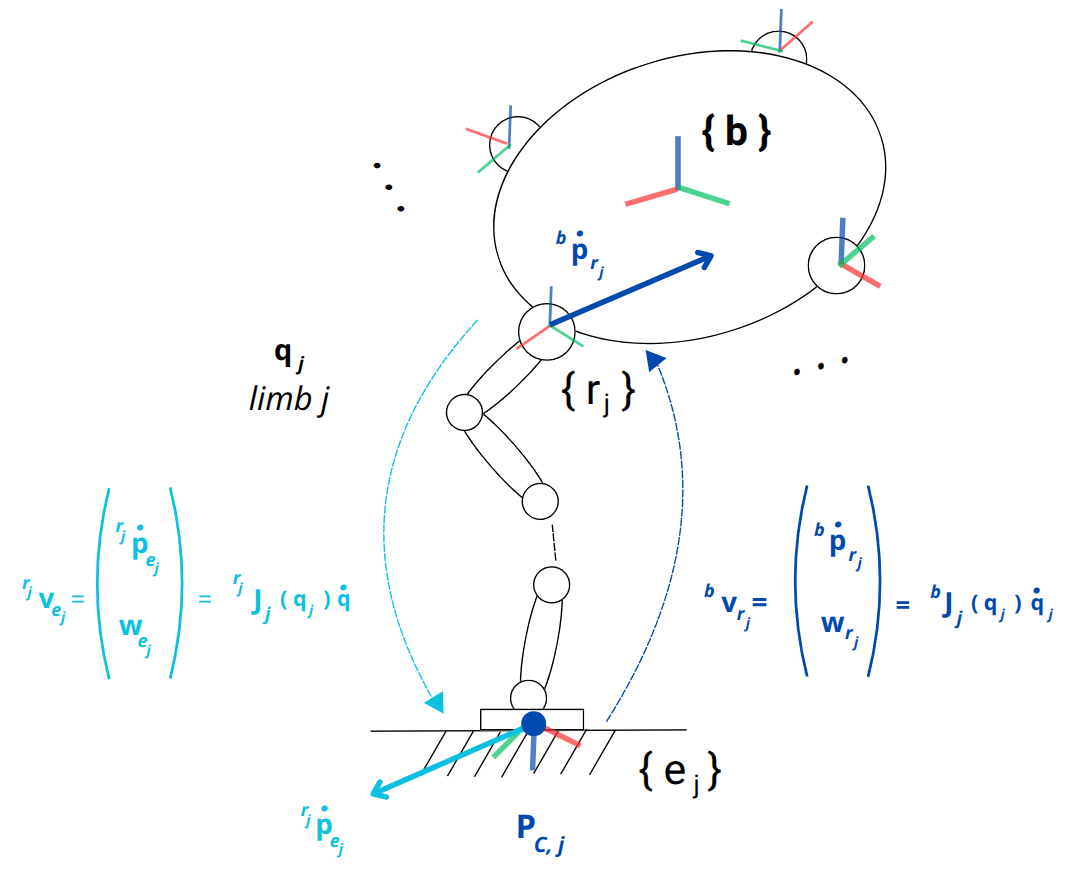
\includegraphics[width=0.6\textwidth]{Images/img_ch3/diffkin_multilimb.png}
    \caption{Schematic representation of single limb differential kinematic relation}
    \label{fig:diffkin_multilimb}
\end{figure}

$\mathbf{h}_a \in \mathbb{R}^{m}$
$\mathbf{h} \in \mathbb{R}^M , M = m\cdot N_c$

The vectors of generalized forces at the limb root, generated from ground contact interaction, are denoted as $\mathbf{h_i} \in \mathbb{R}^m$, and collected as $\mathbf{h} \in \mathbb{R}^M$ ($M = m\cdot N_c$).If the vector of external forces applied at the CoM of the base is denoted as $\mathbf{h_a}$, then: 
\begin{equation}
    \mathbf{h}_a = \mathbf{W} \mathbf{h}
    \label{eq:grasping_relation}
\end{equation}
Where $\mathbf{W} \in \mathbb{R}^{m \times M}$  is the grasping matrix, used to map limbs root interaction to base task space. defined as: 
\begin{equation}
    \mathbf{W} = [ \mathbf{W}_1 \dots \mathbf{W}_j \dots\mathbf{W}_N],\quad
    \begin{cases}
    \mathbf{W}_j = \mathbf{0} \in \mathbb{R}^{m\times m}  \quad \text{if } j\not \in J_c\\
    \mathbf{W}_j = \begin{bmatrix}
        \mathbf{I_3} & \mathbf{0_3} \\
        \mathbf{R}_j & \mathbf{I_3}    \end{bmatrix} 
        , \quad \text{if } j \in J_c
    \end{cases}
    \label{eq:grasping_relation_rev}
\end{equation}

With $\mathbf{R}_j$ responsible of performing the vector product $\mathbf{d}_j \times \mathbf{f_j} = \mathbf{R}_j\mathbf{f}_j$, where $\mathbf{d}_j$ is the vector from base frame to limb $j$ root measured in the base frame, as represented in Fig.\ref{fig:multilimbmodel}.

From the inversion of this relation,
and neglecting the internal forces $\mathbf{h_r} \in \mathbb{R}^{M-m}$, which are representative of the null space of $\mathbf{W}$ 
%as explained in Appendix \ref{ch:appendixB}, 
, it is derived: 
\begin{equation}
    \mathbf{h} = \mathbf{W}^\dag \mathbf{h}_a
    \label{eq:grasping_relation_rev}
\end{equation}
Then, using the same notation introduced in chapter \ref{ch:chapter_two}, Jacobian matrices that relate each limb joint velocities to limb root, in the base frame, are defined as in (\ref{eq:rootDK_baseframe}) (accordingly to \textit{Assumption 1}), as represented for a single limb in Fig.\ref{fig:diffkin_multilimb}.
\begin{equation}
    \label{eq:root_jacobian}
     \mathbf{^b J_j(q_j)} = - \mathbf{J^b_{r_j}}\mathbf{{^{r_j}J_j}(q_j)}
\end{equation}
Where $\mathbf{{^{r_j}J_j}(q_j)}$ is the jacobian matrix of limb $j$, computed considering the limb-tip as EE and the root frame $\mathbf{r_j}$ as the "fixed" base.  
Those Jacobian matrices are collected in 
$\mathbf{J}(\mathbf{q}) \in \mathbb{R}^{M \times n}$ as 
\begin{equation}
\label{eq:JacobianFormulaMultiLimb}
    \mathbf{J}(\mathbf{q}) = diag(\mathbf{^b J_1}(\mathbf{q_1}) \dots \mathbf{^b J_j}(\mathbf{q}_j) \dots \mathbf{^b J_N}(\mathbf{q}_N)) ,\quad
    \mathbf{J_j}(\mathbf{q}_j) = \mathbf{0} \in \mathbb{R}^{m\times n_j}  \quad \text{if } j\not \in J_c
\end{equation}

While joint torque vectors in $\mathbf{\tau} \in \mathbb{R}^n$.
the kinetostatic relation (\ref{eq:Static}) holds, with $\mathbf{\gamma}_e = \mathbf{h}$, so substituting (\ref{eq:grasping_relation}): 

\begin{equation}
    \mathbf{\tau} = \mathbf{J}^T_a(\mathbf{q})\mathbf{h}_a
    \label{eq:MultiLimbKinetostatic}
\end{equation}
Where $\mathbf{J}^T_a(\mathbf{q}) = \mathbf{J}^T(\mathbf{q})\mathbf{W}^\dag \in \mathbb{R}^{n\times m}$

From kinetostatic duality, denoting with $\mathbf{v}_a \in \mathbb{R}^m$, the absolute velocity of the base, it holds the dual of (\ref{eq:MultiLimbKinetostatic}): 
\begin{equation}
    \mathbf{v}_a = \mathbf{J}_a(\mathbf{q})\mathbf{\dot{q}}
    \label{eq:MultiLimbvel}
\end{equation}

Finally, from relation (\ref{eq:MultiLimbvel}) and (\ref{eq:MultiLimbKinetostatic}) the \textit{\textbf{external base force manipulabnility ellipsoid}} for the base (EBFME), and the \textit{\textbf{absolute base velocity manipulability ellipsoid}} (ABVME) are defined as follows: 
\begin{equation}
    \mathbf{h}^T_a [\mathbf{J}_a(\mathbf{q})\mathbf{J}^T_a(\mathbf{q})]\mathbf{h}_a = 1
    \label{eq:BEFME}
\end{equation}
\begin{equation}
    \mathbf{v}^T_a [\mathbf{J}_a(\mathbf{q})\mathbf{J}^T_a(\mathbf{q})]^{-1}\mathbf{v}_a = 1
    \label{eq:ABVME}
\end{equation}

The matrix $\mathbf{E}_a \in \mathbb{R}^{m\times m}$ represents the core of the EBFME's quadratic form, while its inverse is the ABVME's. 
When the limbs have at least 6 DOFs, $m = 6$ (task space includes both rotation and translation), and a 6-dimensional curve clearly cannot be visualized, but a numeric index like the manipulability measure proposed by Yoshikawa \cite{ManipulabilityYoshikawa} can be defined:
\begin{equation}
\label{eq:ManipulabilityMeasureBase}
    w_a(\mathbf{q}) = \sqrt{det(\mathbf{E}_a(\mathbf{q}}))
\end{equation}

From now on, the joints' dependency is implicit.
By analyzing the equation of the ellipsoid matrix, and decomposing the absolute base Jacobian matrix, it is possible to decompose also $\mathbf{E}_a$ in a translational and rotational part. Denoting with $m_P \leq 3$ the dimension of the translational task space, and $m_O \leq 3$ for the rotational one ($m = m_O + m_P \leq 6$), the base Jacobian is decomposed in its translational  ($\mathbf{J_P}_a \in \mathbb{R}^{m_P \times n}$) and rotational part($\mathbf{J_O}_a \in \mathbb{R}^{m_O \times n}$): 
$\textbf{J}_a = \begin{bmatrix}
    \mathbf{J_P}_a\\ \mathbf{J_O}_a
\end{bmatrix}$ 
Then the expression of the ellipsoid matrix is: 
\begin{equation}
\label{eq:BME_decoupled}
    \mathbf{E}_a = \begin{bmatrix}
        \mathbf{E_T}_a & \mathbf{E_{TR}}_a \\
        \mathbf{E^T_{TR}}_a & \mathbf{E_{R}}_a 
    \end{bmatrix}
\end{equation}
Where $\mathbf{E_T}_a \in \mathbb{R}^{m_P \times m_P}$ is the core of the translational BME (TBME),  
$\mathbf{E_R}_a \in \mathbb{R}^{m_O \times m_O}$
is the core of the rotational BME (RBME),
and $\mathbf{E_{TR}}_a \in \mathbb{R}^{m_P \times m_O}$ is a coupling matrix.

If decoupling is possible, translational motion is analyzed with $\mathbf{E_T}_a$, while rotational with $\mathbf{E_R}_a$, furthermore, information could be derived from the coupling matrix. When the complete decoupling cannot be proven, an approximation can be used.

Yoshikawa studied the decoupling of translational and rotational manipulability \cite{TRManipulability}, sometimes implicit in the robotic structure, as in spherical wrist manipulators  (where the three wrist joints meet in a single point). When the mechanical structure doesn't imply it, a rule of thumb can be used to measure the quality of the approximation.
For example, the ratio of the matrix norms
\begin{equation*}
z_T = \frac{{||\mathbf{E_T}_a||}_2}{{||\mathbf{E_{TR}}_a||}_2} \quad
z_R = \frac{{||\mathbf{E_R}_a||}_2}{{||\mathbf{E_TR}_a||}_2} 
\end{equation*}
When the ratio of the motion under analysis is big enough, the coupling is negligible and the approximation is possible. 
Then, even when $m = 6$, the overall EM $\mathbf{E_a}$ is decomposed in its components, and independent analysis of translational or rotational motion is possible.
In this case, the ABVME can be decomposed in translational (ATBVME) and rotational (ARBVME):
\begin{equation}
    \mathbf{\dot{p}}^T_a [\mathbf{E_T}_a]^{-1}\mathbf{\dot{p}}_a = 1
    \label{eq:ATBVME}
\end{equation}
\begin{equation}
    \mathbf{\omega}^T_a [\mathbf{E_R}_a]^{-1}\mathbf{\omega}_a = 1
    \label{eq:ARBVME}
\end{equation}

Next, this theory is applied to multi-limbed robots, computing the ATBVME and analyzing its meaning.

\subsection{Multi-limb Robots ME Examples and Extensions}
\label{sec:ME_multi_limb_example}

An intuitive description of the manipulability ellipsoid is useful for understanding the examples and results discussed in the next.

T.Yoshikawa\cite{TRManipulability} proposes the manipulability ellipsoid as a measure of "ease of arbitrary changing the position and orientation of the end effector at the rip of the manipulator". Defined by the mapping of a unit sphere in the velocity (force) joint space to the corresponding velocity (force) task space, resulting in an ellipsoid. By looking at the major axis of the ellipsoid, it suggests the direction in which the mechanical system performs better. In fact, the distance between the ellipsoid center and its surface is a measure of how the joint space unit sphere is mapped in the task space, then, it is a measure of the "transformation ratio".
S.L.Chiu describes\cite{TaskCompatibilityPosture} this relation by interpreting the manipulator as a mechanical transformer with joint velocity (force) as input and Cartesian velocity (force) as output. 

Furthermore, from kinetostatic duality, it can be proven that the matrix describing the quadratic form of the velocity and manipulability ellipsoids are one the inverse of the other. That means that the maximum VME axis corresponds to the minimum FME axis. 
With the mechanical transformer interpretation, the conservation of energy justifies the F/VME duality, as amplification in velocity transmission corresponds to a reduction in force transmission, and vice versa\cite{TaskCompatibilityEllipsoid}.

With this simple interpretation (rather than the equations previously derived), it is clear that the closer the VME is to a sphere, the better the end-effector can move isotropically along all task space directions \cite{Siciliano}. When the VME gets elongated along some directions, those are the preferred directions of motion, 
and in the limit case when one axis becomes null, task space mobility is lost in that direction, and the system is in a singular configuration. 

If the extension of the manipulability theory is correct, similar considerations should hold for multi-limbed robot base motion. 
Even if the BME is the main objective, from the aspects described above, it can be deduced that the manipulability theory is useful also in analyzing the performance of limbs on their own. Concepts of task compatibility\cite{TaskCompatibilityPosture} and ellipsoid tracking \cite{EllipsoidTracking} can be employed when defining limb tasks such as manipulation, grasping configuration while climbing, or the best direction to approach the ground.
Furthermore, When using a complex EE such as GRIEEL, optimal postures in wheel mode can be defined based on the ellipsoid shape, according to driving requirements in interacting with the ground. 



As a final consideration, the V/FME is a powerful tool not only for its intuitive interpretation but also for the ease of computation, which comes from the singular value decomposition of the manipulator Jacobian matrix\cite{Siciliano}\cite{YoshikawaRoboticsBook}. 
However, it presents some limitations a lot discussed in literature\cite{PolytopesManipulability}\cite{LimitsEllipsoid}, one of those is the unrealistic hypothesis of the hypershpere joint velocity domain $||\dot{\mathbf{q}}|| = \dot{\mathbf{q}}^T\dot{\mathbf{q}}\leq 1$, a polytope ( $-\dot{q}_{i,max} \leq \dot{q}_i \leq \dot{q}_{i,max}, i=1,\dots,n$) is usually a better domain.

Despite this limitation, results obtained by applying the VME theory to some multi-limbed robots provide usefull information, both for mechanical design and the configuration definition during task execution, as discussed now. 

The following examples are implemented in MATLAB, with base manipulability theory and multi-limbed robots' kinematic computation. The used code is open-source, and it can be found in this \href{https://github.com/AlePuglisi/limbed-robot-control}{GitHub} repository.

\subsubsection{Example 1: Quadruped with 3-DOFs Limbs}
\label{sec:BME_quadruped}

This example considers a simple 4-limbed robot where each limb has 3 DOFs anthropomorphic arm configuration (as the one in Fig.\ref{fig:antropomorphicDH}), and an insect leg topology\cite{Todd}\cite{KentaroUnoPhD}. 
Even if the anthropomorphic configuration is considered (attached to the base), the leg links are denoted in order as coxa, femur, and tibia, with joints B2C, C2F, and F2T. 
From now on, this robot will be called LimbedEx1. 
The DH parameters of the limb are reported in Tab.\ref{table:limb_ex1_1_DH}, and the robot is represented in Fig.\ref{fig:ex1_robot}, with all legs in the zero configuration $\mathbf{q_0} = \begin{bmatrix}
    0 & 0 & 0
\end{bmatrix}^T$ and in the initial walking configuration $\mathbf{q_W} = \begin{bmatrix}
    0 & -\pi/6 & \frac{2}{3}\pi
\end{bmatrix}^T$.

\begin{figure}[H]
    \centering
    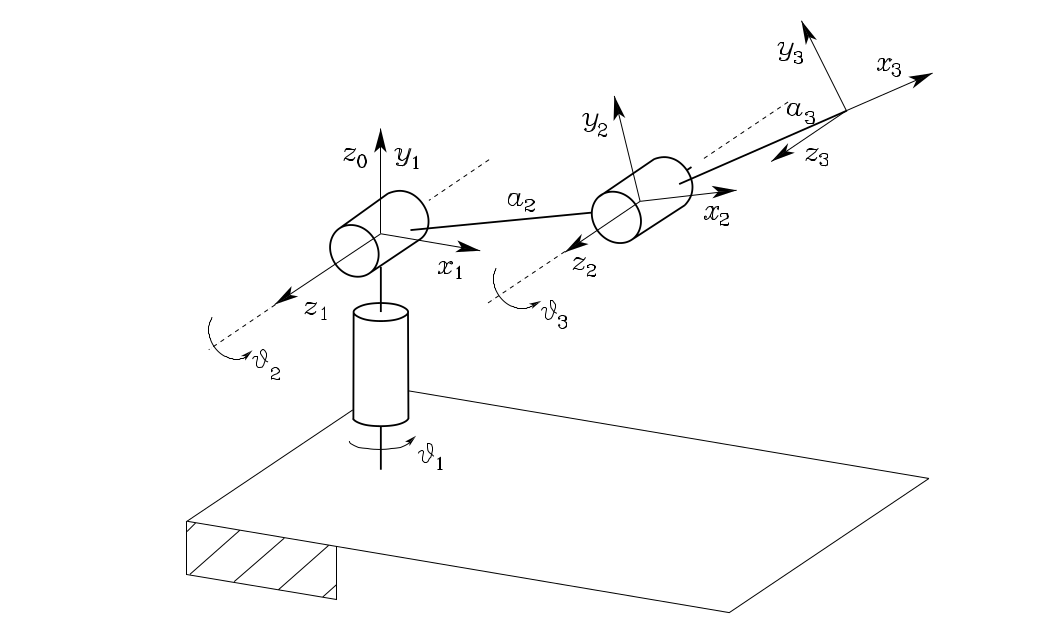
\includegraphics[width=0.6\textwidth]{Images/img_ch3/antropomorphicDH.png}
    \caption{\cite{Siciliano} representation of an anthropomorphic arm, with DH frames}
    \label{fig:antropomorphicDH}
\end{figure}

\begin{table}[H]
\centering 
    \caption{LimbedEx1 DH parameters}
    \label{table:limb_ex1_1_DH}
    \begin{tabular}{| l | c | c | c | c | c |}
    \hline
    \rowcolor{bluepoli!40}
%    \rowcolor{bluepoli!40}
     \textbf{Link} &  $a_i$ $[m]$ & $\alpha_i$ $[rad]$ & $d_i$ $[m] $ & $\theta_i$ $[rad]$ & $\theta_{offset, i}$ $[rad]$ \T\B \\
    \hline \hline
    \textbf{Coxa} ($i=1$) & 0.0 & $-\frac{\pi}{2}$ & 0.1  & $q_1$  & 0.0 \T\B\\
    \hline 
    \textbf{Femur} ($i=2$) & 0.35 & 0.0  & 0.0  & $q_2$  & 0.0  \T\B\\
    \hline
    \textbf{Tibia} ($i=3$) & 0.35  & 0.0  & 0.0  & $q_3$ & 0.0 \T\B\\
    \hline
    \end{tabular}
\end{table}

\begin{figure}[H]
    \centering
    \subfloat[LimbedEx1 with limbs in $\mathbf{q_0}$\label{fig:quadruped_q0}]{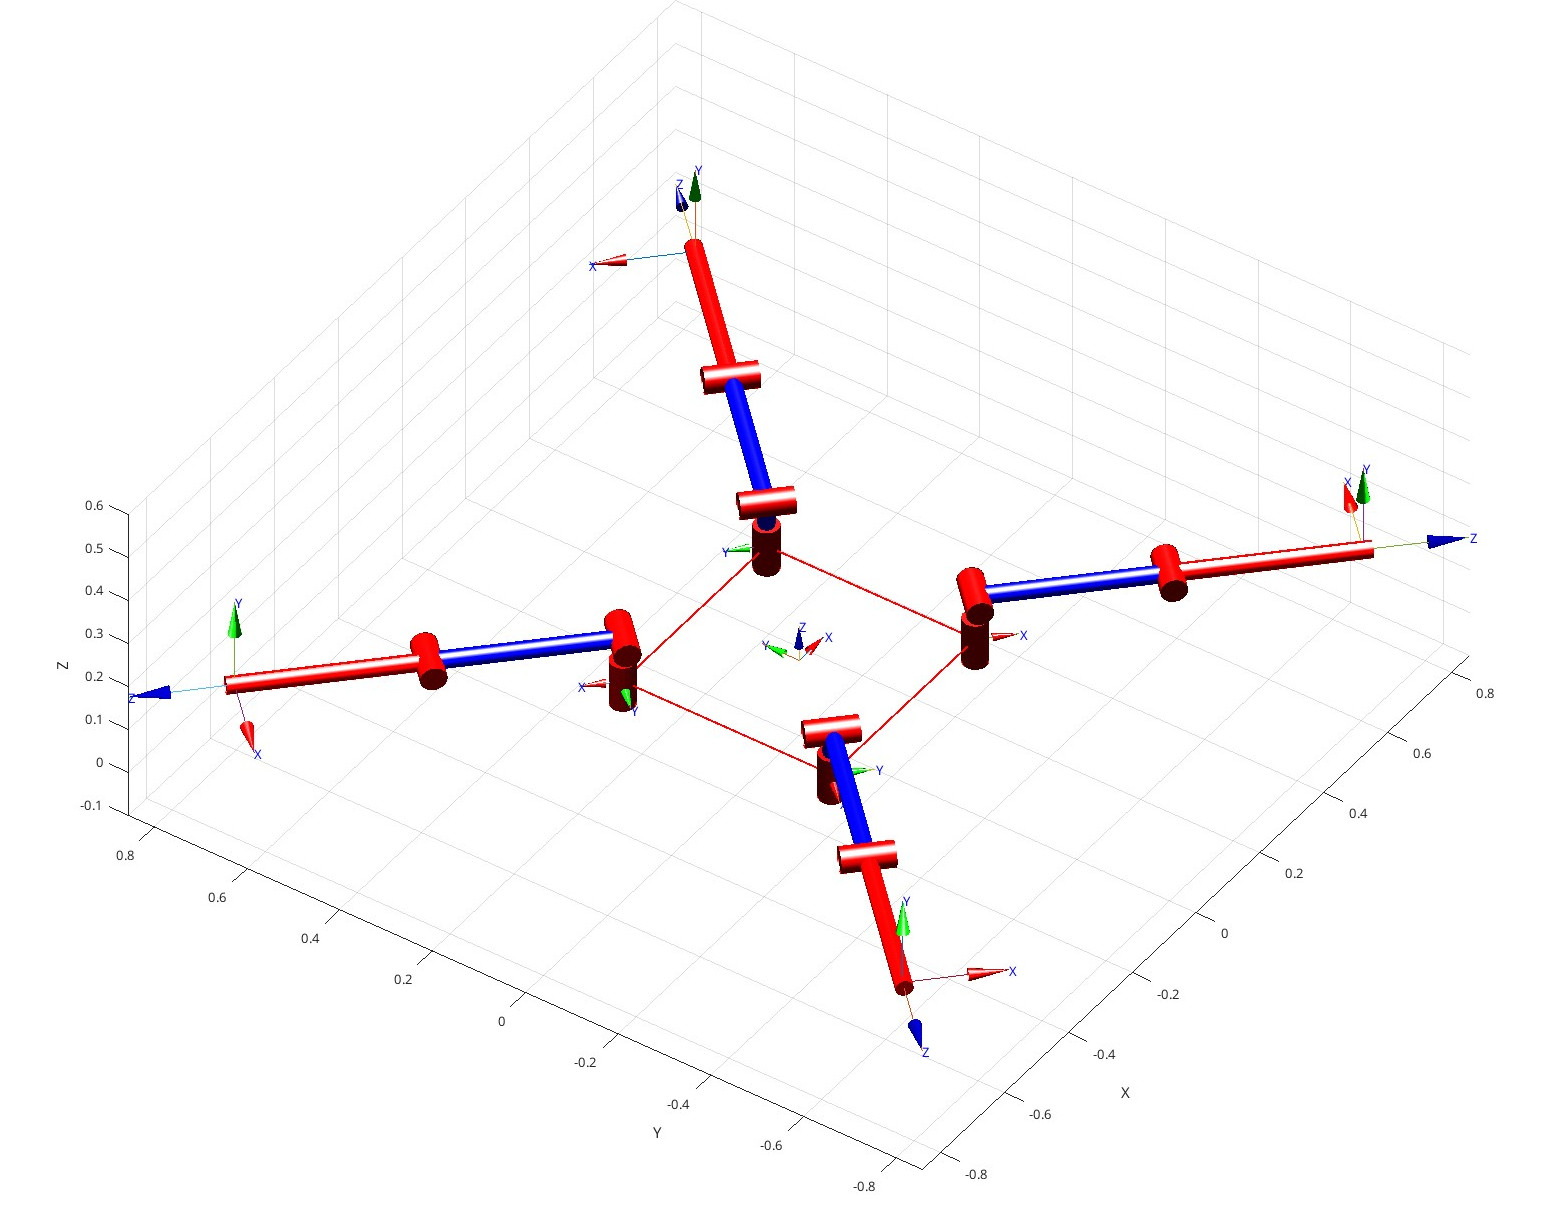
\includegraphics[width=0.45\textwidth]{Images/img_ch3/quadruped_q0.jpg}}
    \subfloat[LimbedEx1 with limbs in $\mathbf{q_W}$\label{fig:quadruped_qw}]{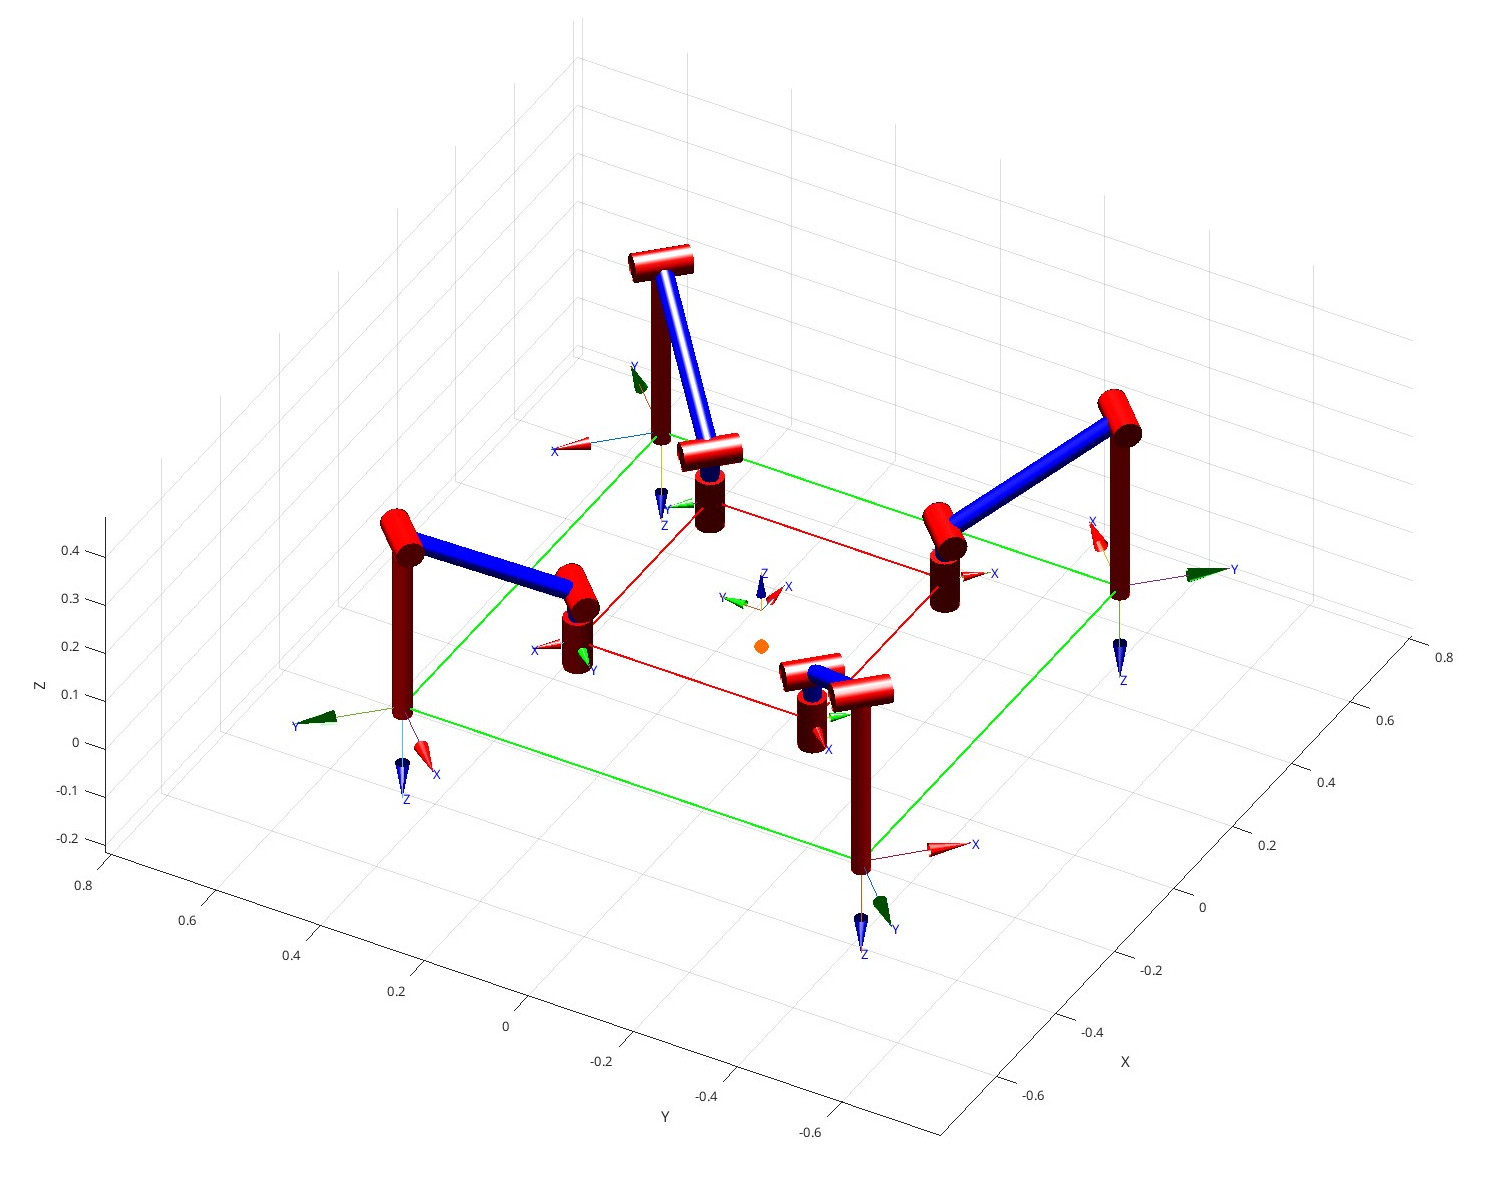
\includegraphics[width=0.45\textwidth]{Images/img_ch3/quadruped_qw.jpg}} 
    \caption[LimbedEx1 in zero and walking configuration]{LimbedEx1 in zero and walking configuration}
    \label{fig:ex1_robot}
\end{figure}

The results of the TVME of each limb and the ATBVME are now reported in different configurations.
Each limb TVME is represented to understand how they affect base motion, but also because the manipulability of the limb gives information on how it can interact with the environment when manipulating or approaching the ground, as described before. 

The figures will use the following convention: 
\begin{itemize}
    \setlength\itemsep{-0.7em} 
    \item\textbf{Robot torso}: Red polygon (connecting limb roots).
    \item\textbf{Base CoM}($\mathbf{P_CoM}$): Positioned in the base frame center.
    \item\textbf{Base CoM Projection}($\mathbf{\overline{P_CoM}}$): Orange point.
    \item\textbf{Support pattern}: Green polygon (connecting contact points). 
    \item\textbf{ATBVME}: Red ellipsoid (in the base frame). 
    \item\textbf{Contact limbs VME}: Blue ellipsoids (in the limbs EE frame). 
    \item\textbf{Contact limbs VME}: Green ellipsoids (in the limbs EE frame). 
\end{itemize}

The different configurations analyzed are computed as results of base motion translation tasks from the walking configuration, considering possible limb raises.

\textbf{Walking Configuration}
\begin{figure}[H]
    \centering
    \subfloat[perspective view\label{fig:ex1_walking_ortho}]{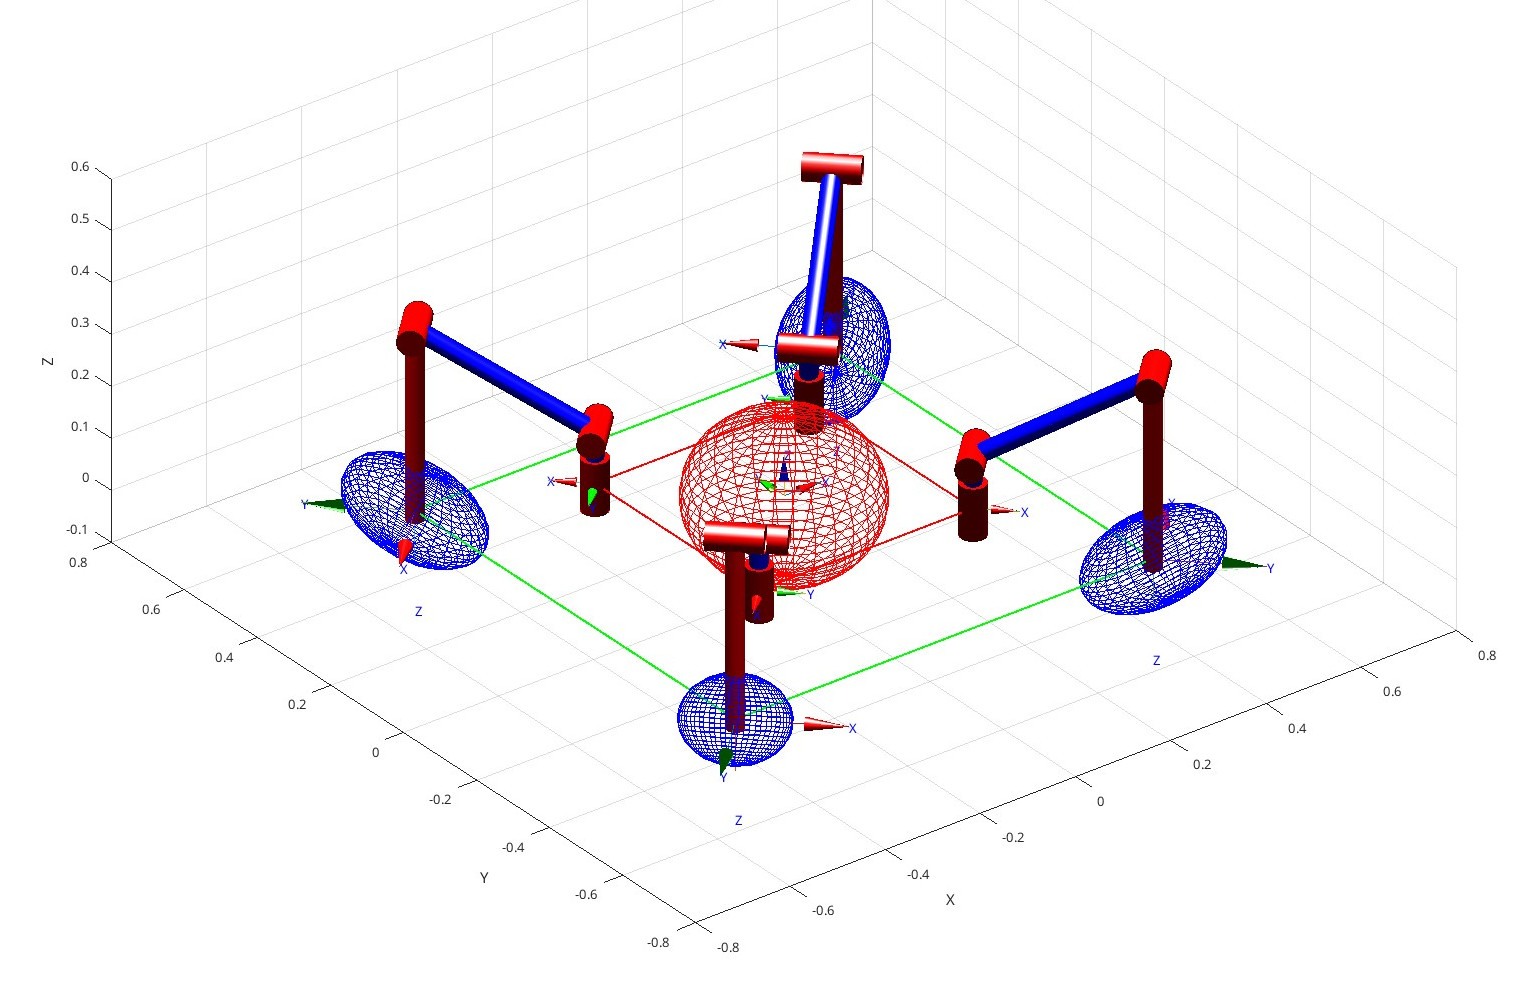
\includegraphics[width=0.3\textwidth]{Images/img_ch3/ex1_walking_ortho.jpg}}
    \subfloat[xy view\label{fig:ex1_walking_xy}]{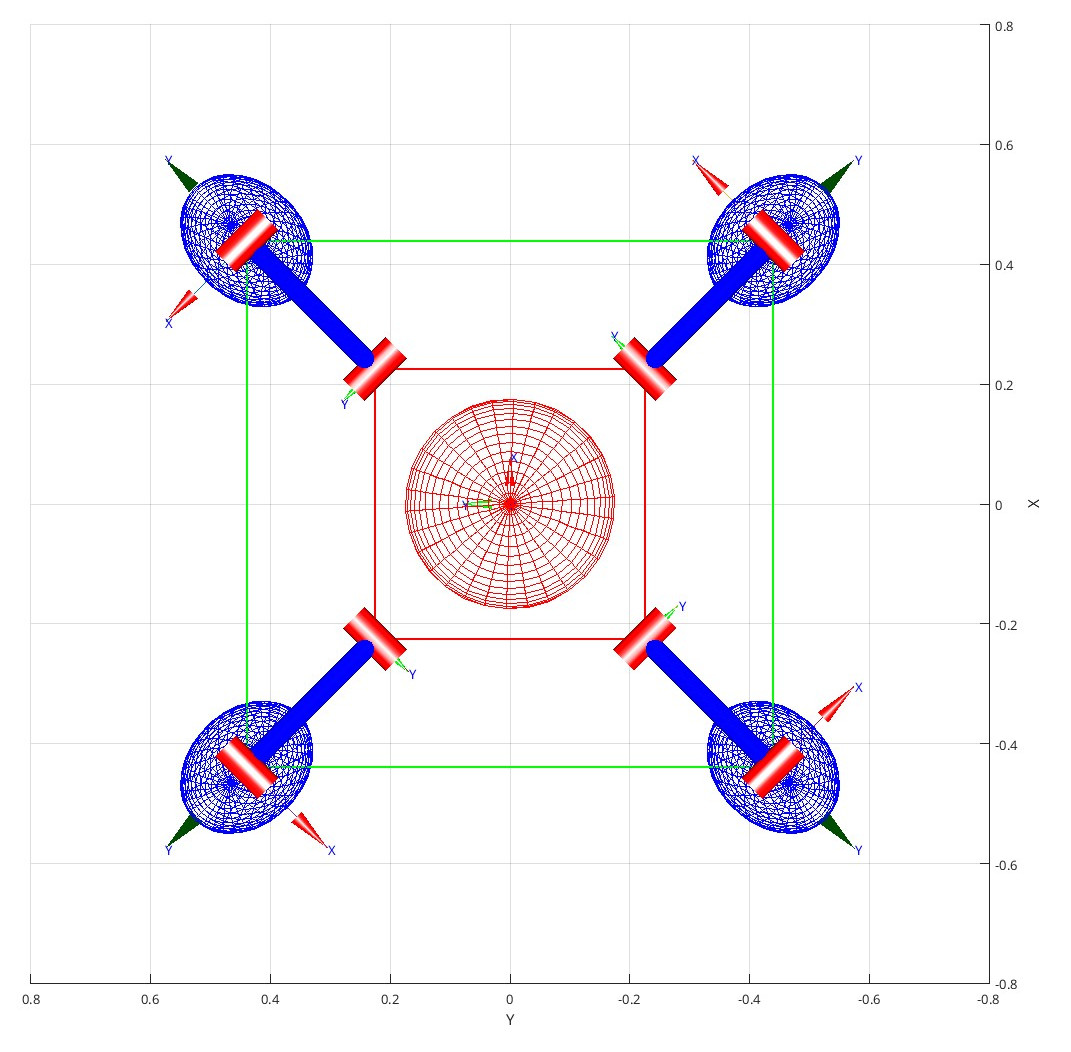
\includegraphics[width=0.3\textwidth]{Images/img_ch3/ex1_walking_xy.jpg}} 
    \subfloat[xz view\label{fig:ex1_walking_xz}]
    {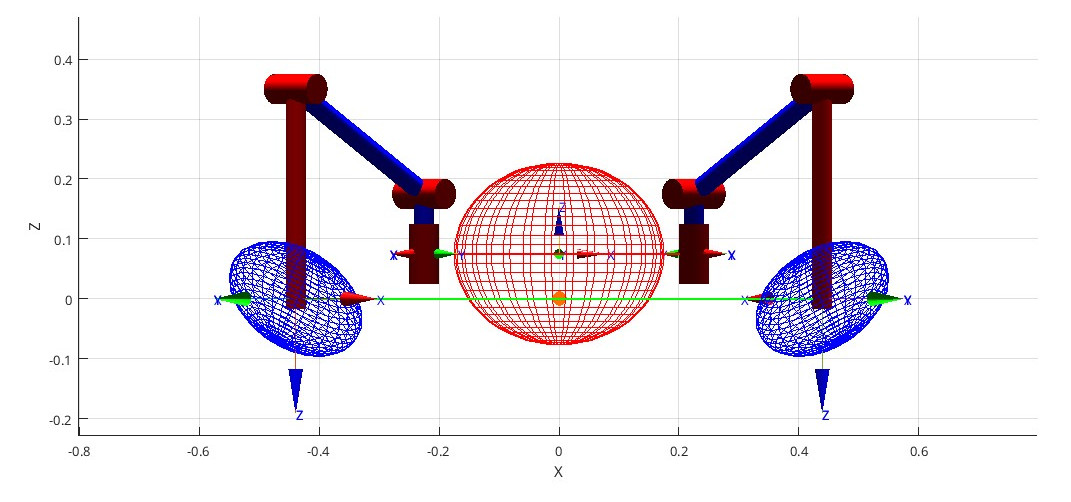
\includegraphics[width=0.3\textwidth]{Images/img_ch3/ex1_walking_xz.jpg}} 
    \caption[LimbedEx1 ME in walking configuration]{LimbedEx1 ME in walking configuration}
    \label{fig:ex1_walking}
\end{figure}

The characteristic isotropic shape of the ATBVME in Fig.\ref{fig:ex1_walking} is coherent with the expected mobility of the robot in this symmetric configuration, where motion in all directions is possible with the same dexterity.  

\textbf{Base z translations}

In this analysis, the manipulability measure is not explicitly reported. Still, recalling that it is proportional to the volume of the ellipsoid, it is simple to deduce how it is changing.

In those first tests, when the base translates along the positive z-axis, the shape of the ellipsoid gets flattened vertically, because of less mobility of the limbs in pushing the ground. This aspect of the ellipsoid axis relative dimensions is consistent, but the first problem of the BME theory is evident from the results in Fig.\ref{fig:ex1_z}. When the base is higher, the ellipsoid is stretched along the xy plane more than flattened in the z-axis, resulting in higher mobility. 
It is evident that "the higher the better" is not accurate when analyzing the dexterity of the base. 


\begin{figure}[H]
    \centering
    \subfloat[z=0.2, perspective view\label{fig:ex1_z020_xy}]{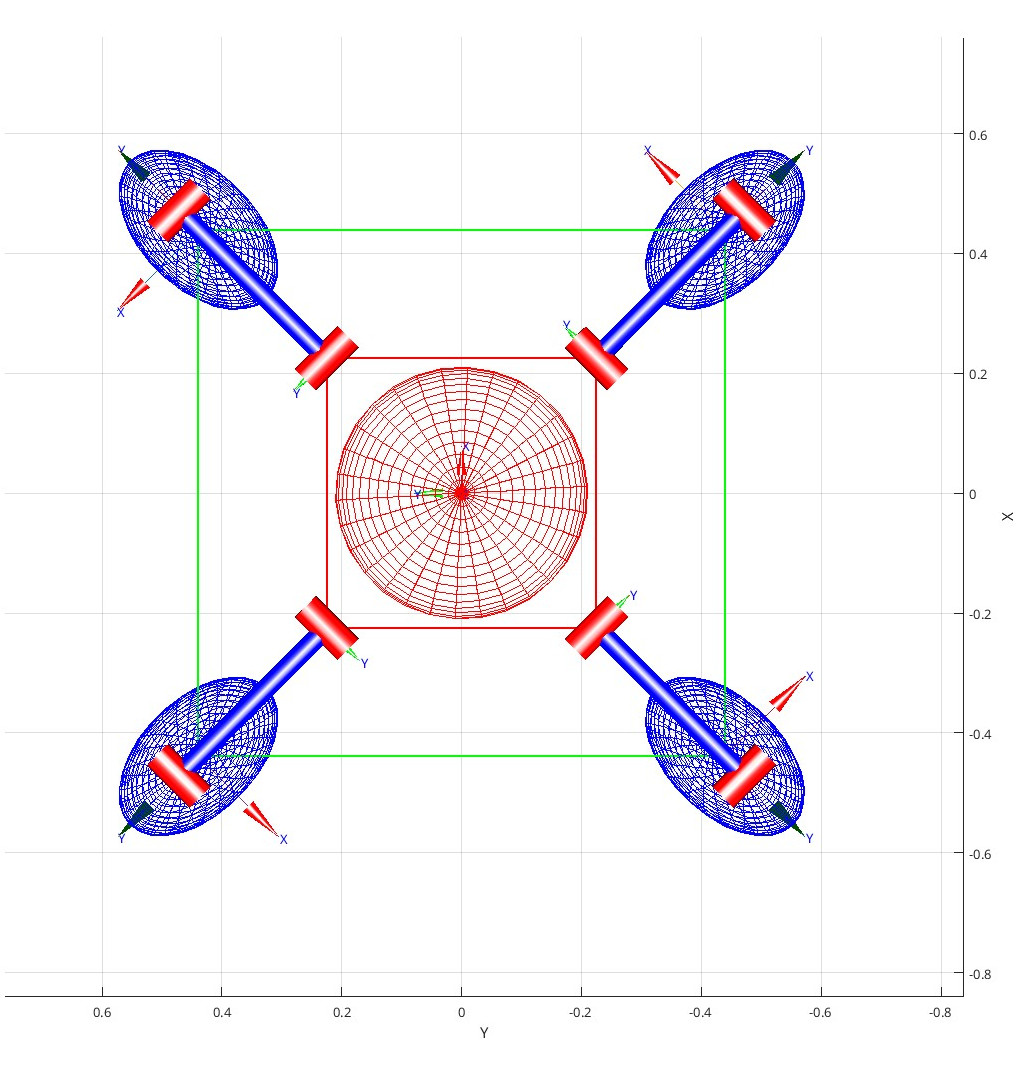
\includegraphics[width=0.35\textwidth]{Images/img_ch3/ex1_z020_xy.jpg}}
    \subfloat[z=0.2, xy view\label{fig:ex1_z020_xz}]{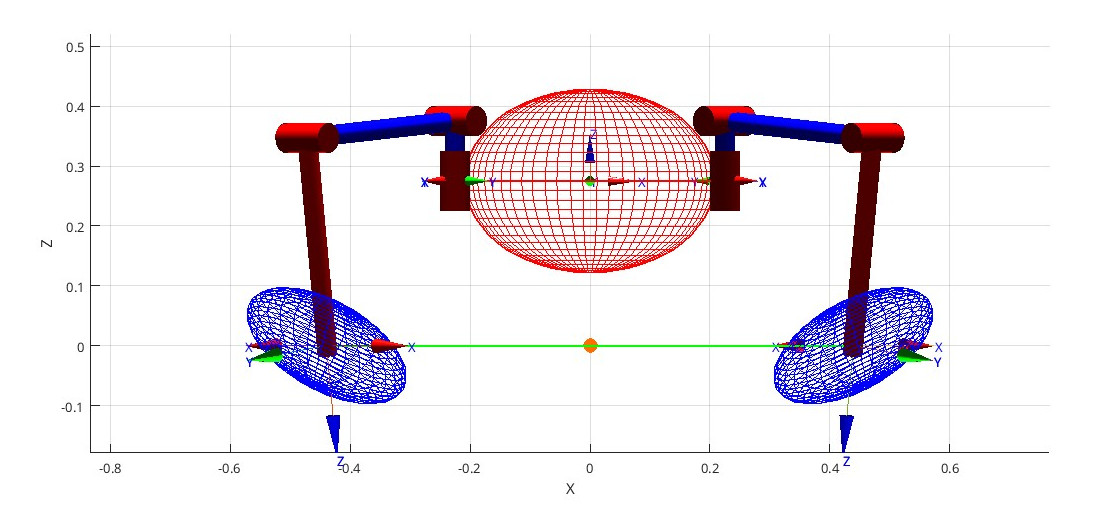
\includegraphics[width=0.35\textwidth]{Images/img_ch3/ex1_z020_xz.jpg}} \\
    \subfloat[z=0.4, xz view\label{fig:ex1_z040_xy}]
    {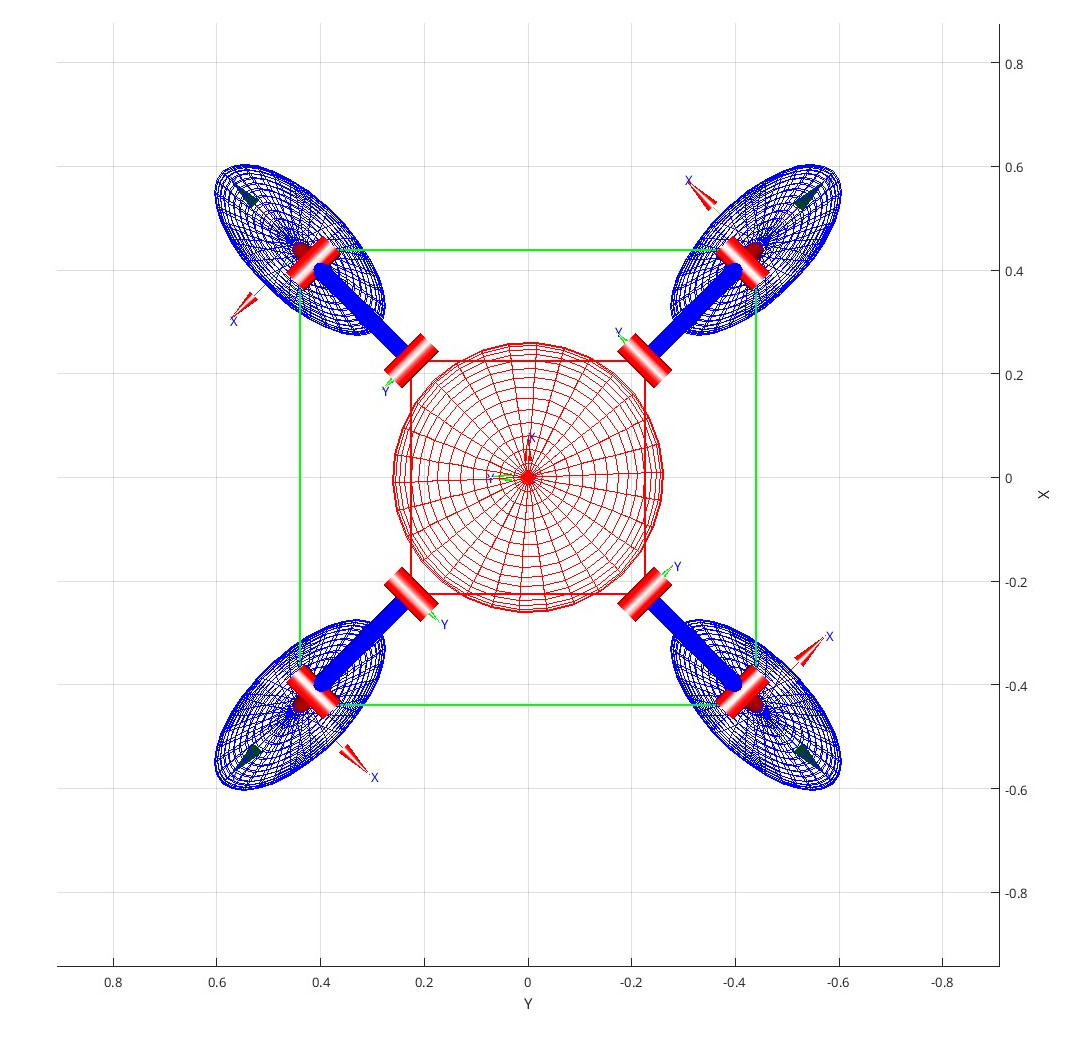
\includegraphics[width=0.35\textwidth]{Images/img_ch3/ex1_z040_xy.jpg}} 
    \subfloat[z=0.4, xz view\label{fig:ex1_z040_xz}]
    {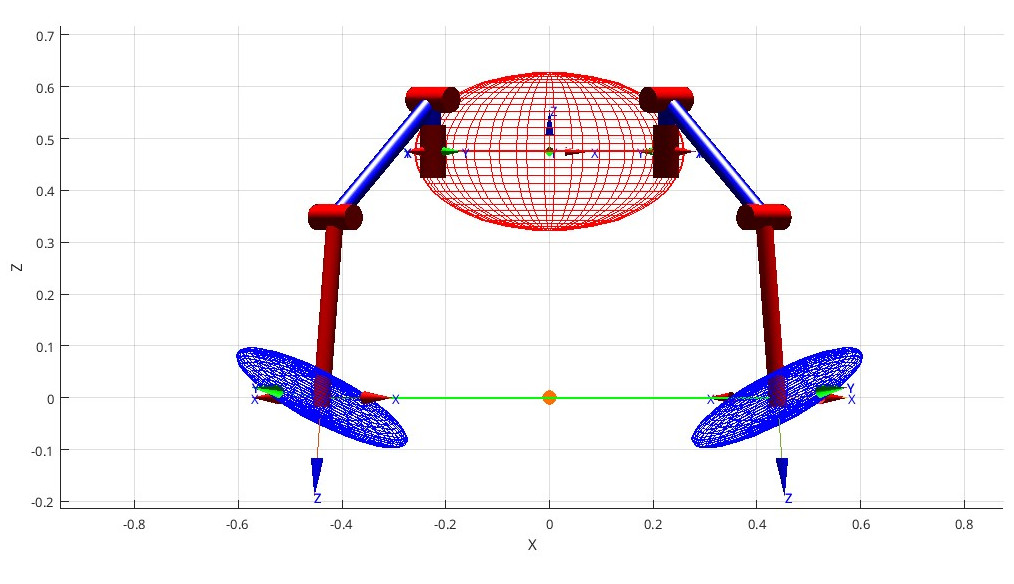
\includegraphics[width=0.35\textwidth]{Images/img_ch3/ex1_z040_xz.jpg}} 
    \caption[LimbedEx1 ME after z base translation]{LimbedEx1 ME after z base translation}
    \label{fig:ex1_z}
\end{figure}

\textbf{Base x,y,z translations}

Translating the base as in Fig.\ref{fig:ex1_xyz_translate} provides again coherent results in the sense of preferred motion directions, with the maximum axis of the ellipsoid orientated where the retracted limbs have a higher range of motion. But again the problem of the quantitative manipulability index is present, and even uncommon configurations such as the one in Fig.\ref{fig:ex1_z01_xneg01_yneg03_xy} result in satisfactory mobility. 

\begin{figure}[H]
    \centering
    \subfloat[z=0.1, x=0.15, xy view\label{fig:ex1_z01_x015_xy}]{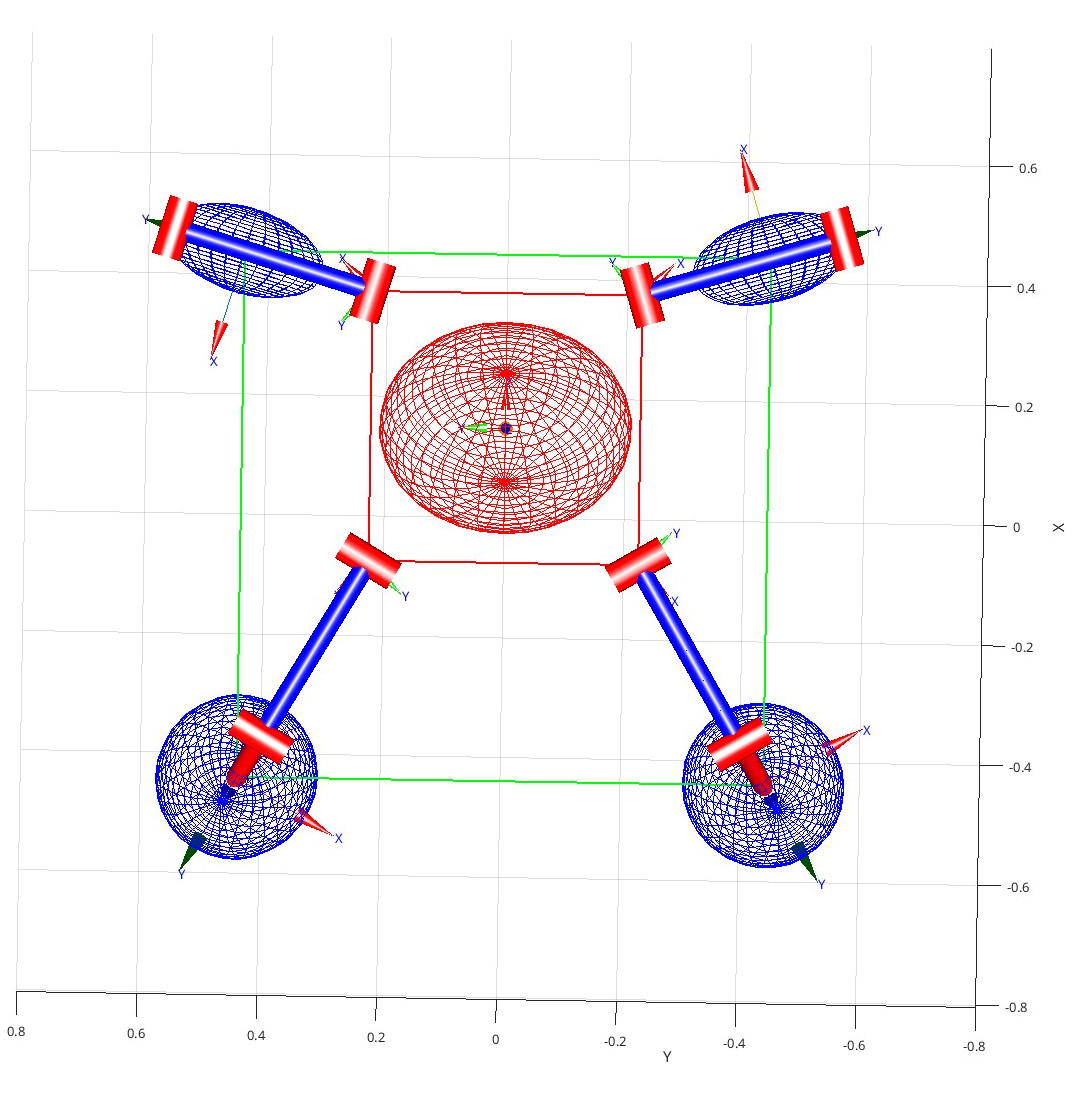
\includegraphics[width=0.35\textwidth]{Images/img_ch3/ex1_z01_x015_xy.jpg}}
    \subfloat[z=0.1, x=0.15, xz view\label{fig:ex1_z01_x015_xz}]{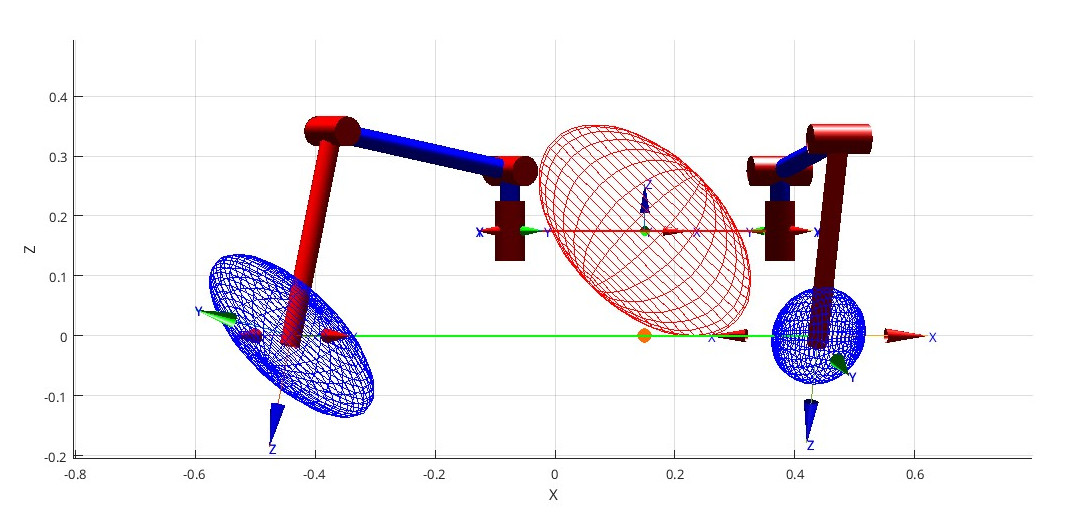
\includegraphics[width=0.35\textwidth]{Images/img_ch3/ex1_z01_x015_xz.jpg}} \\
    \subfloat[z=0.1, x=-0.1, y=-0.3, xy view\label{fig:ex1_z01_xneg01_yneg03_xy}]
    {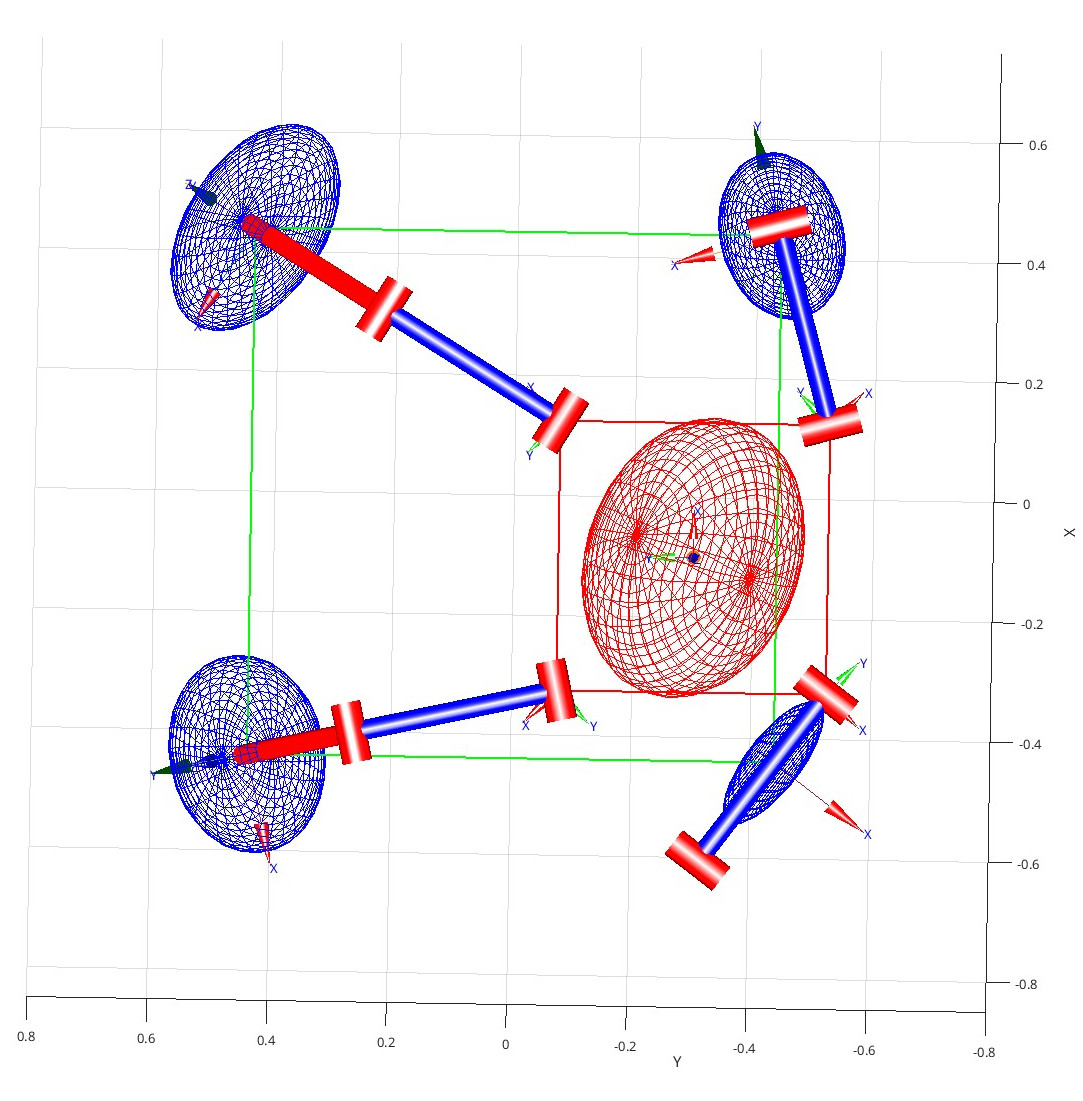
\includegraphics[width=0.35\textwidth]{Images/img_ch3/ex1_z01_xneg01_yneg03_xy.jpg}} 
    \subfloat[z=0.1, x=-0.1, y=-0.3, yz view\label{fig:ex1_z01_xneg01_yneg03_yz}]
    {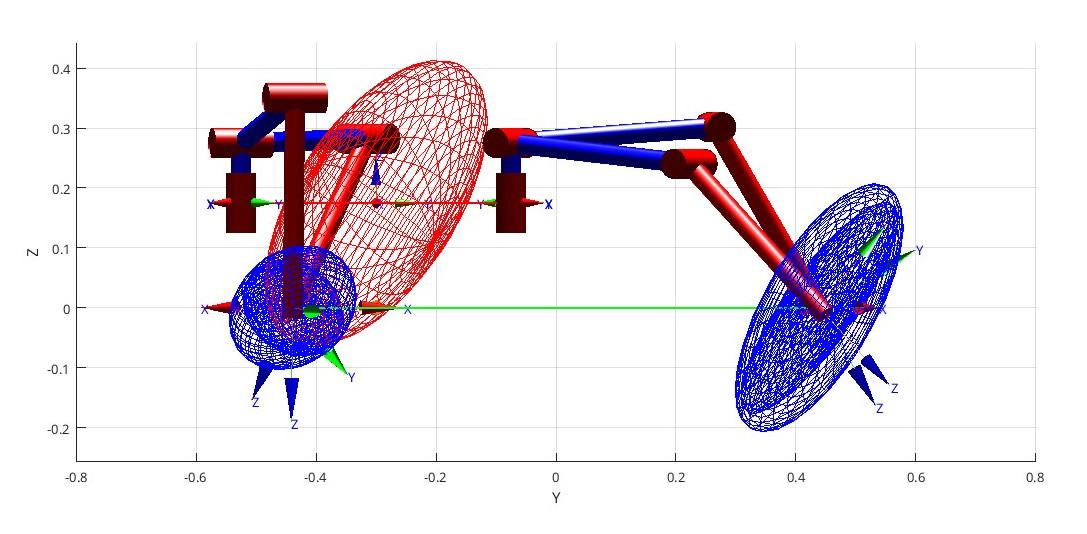
\includegraphics[width=0.35\textwidth]{Images/img_ch3/ex1_z01_xneg01_yneg03_yz.jpg}} 
    \caption[LimbedEx1 ME after generic base translation]{LimbedEx1 ME after generic base translation}
    \label{fig:ex1_xyz_translate}
\end{figure}

\textbf{Raise Limb}
When one limb is raised, only three limbs are used to move the base, and this is reflected in the distorted shape of the ellipsoid.
\begin{figure}[H]
    \centering
    \subfloat[z=0.1, and LF up, perspective view \label{fig:ex1_z01_LFup_ortho}]{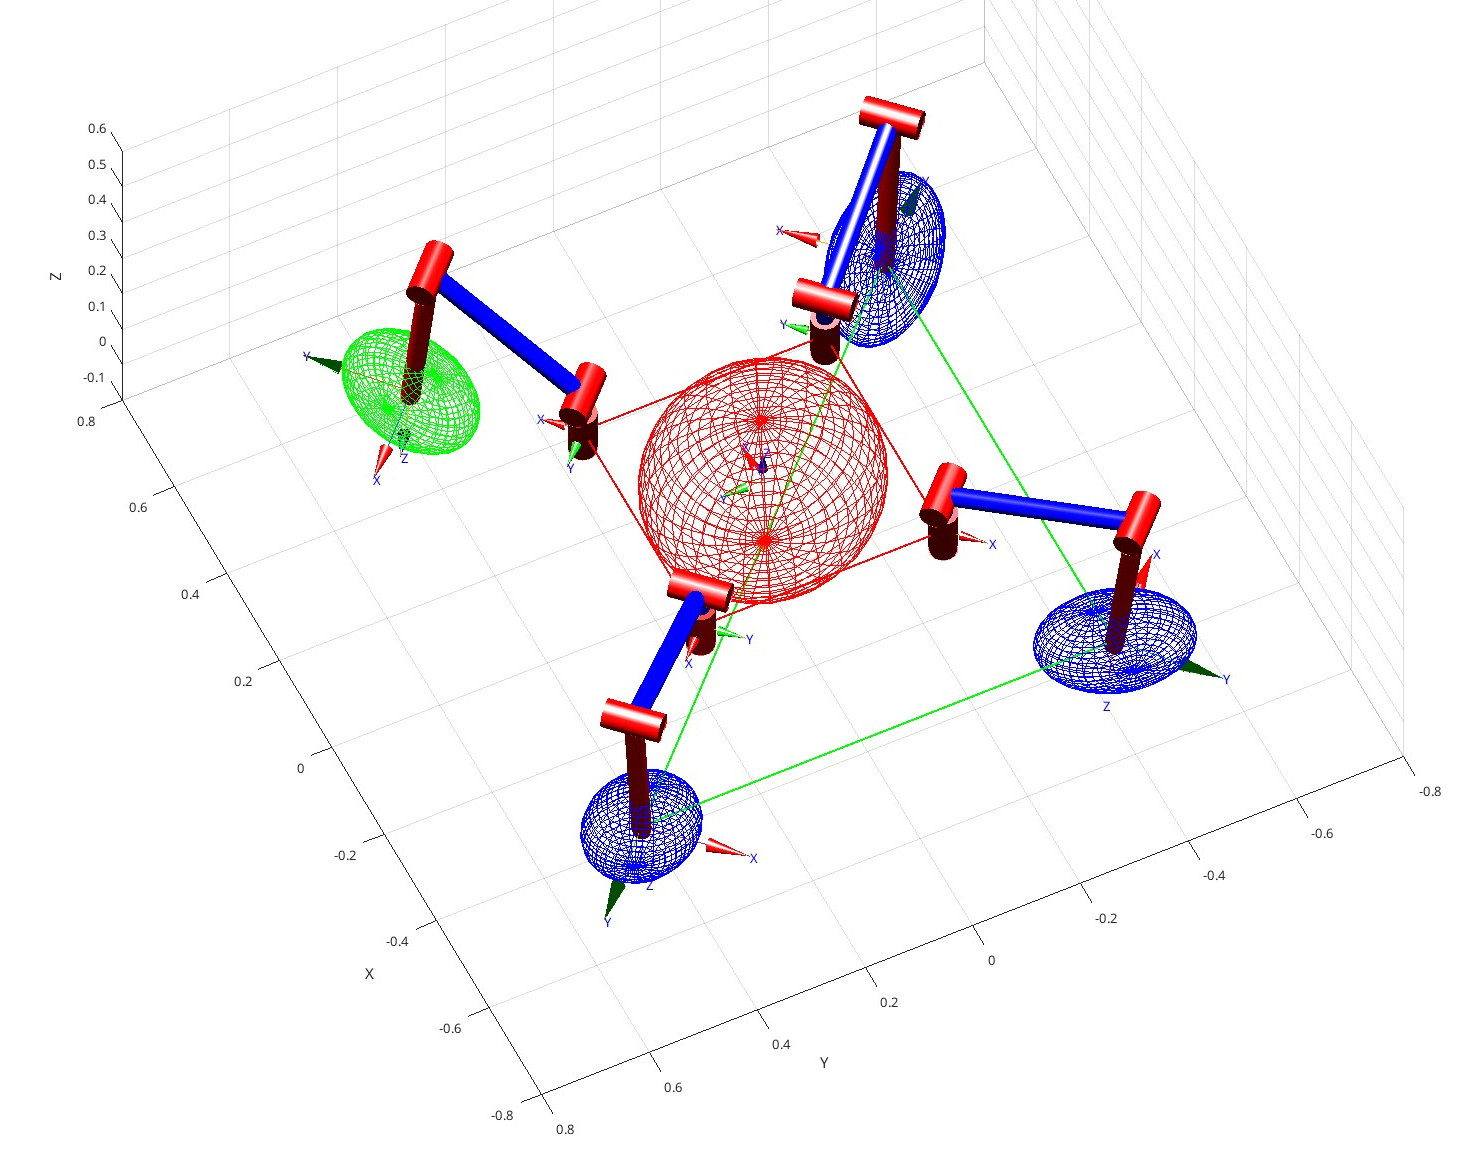
\includegraphics[width=0.35\textwidth]{Images/img_ch3/ex1_z01_LFup_ortho.jpg}}
    \subfloat[z=0.1, and LF up, xy view \label{fig:ex1_z01_LFup_xy}]{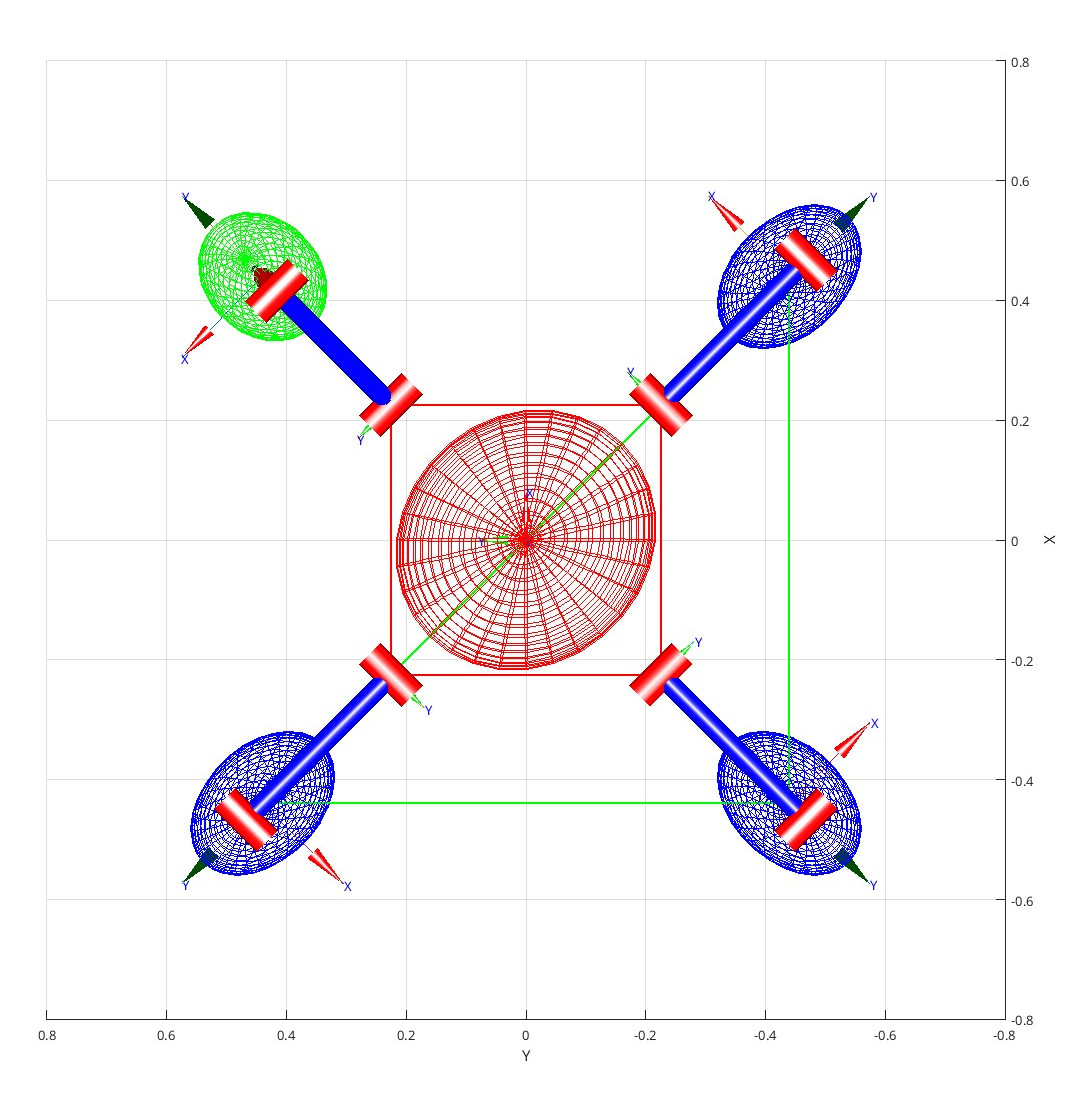
\includegraphics[width=0.35\textwidth]{Images/img_ch3/ex1_z01_LFup_xy.jpg}} \\
    \subfloat[z=0.1, x=-0.1, y=-0.1, and LF up, perspective view \label{fig:ex1_z01_xneg01_yneg01_LFup_ortho}]{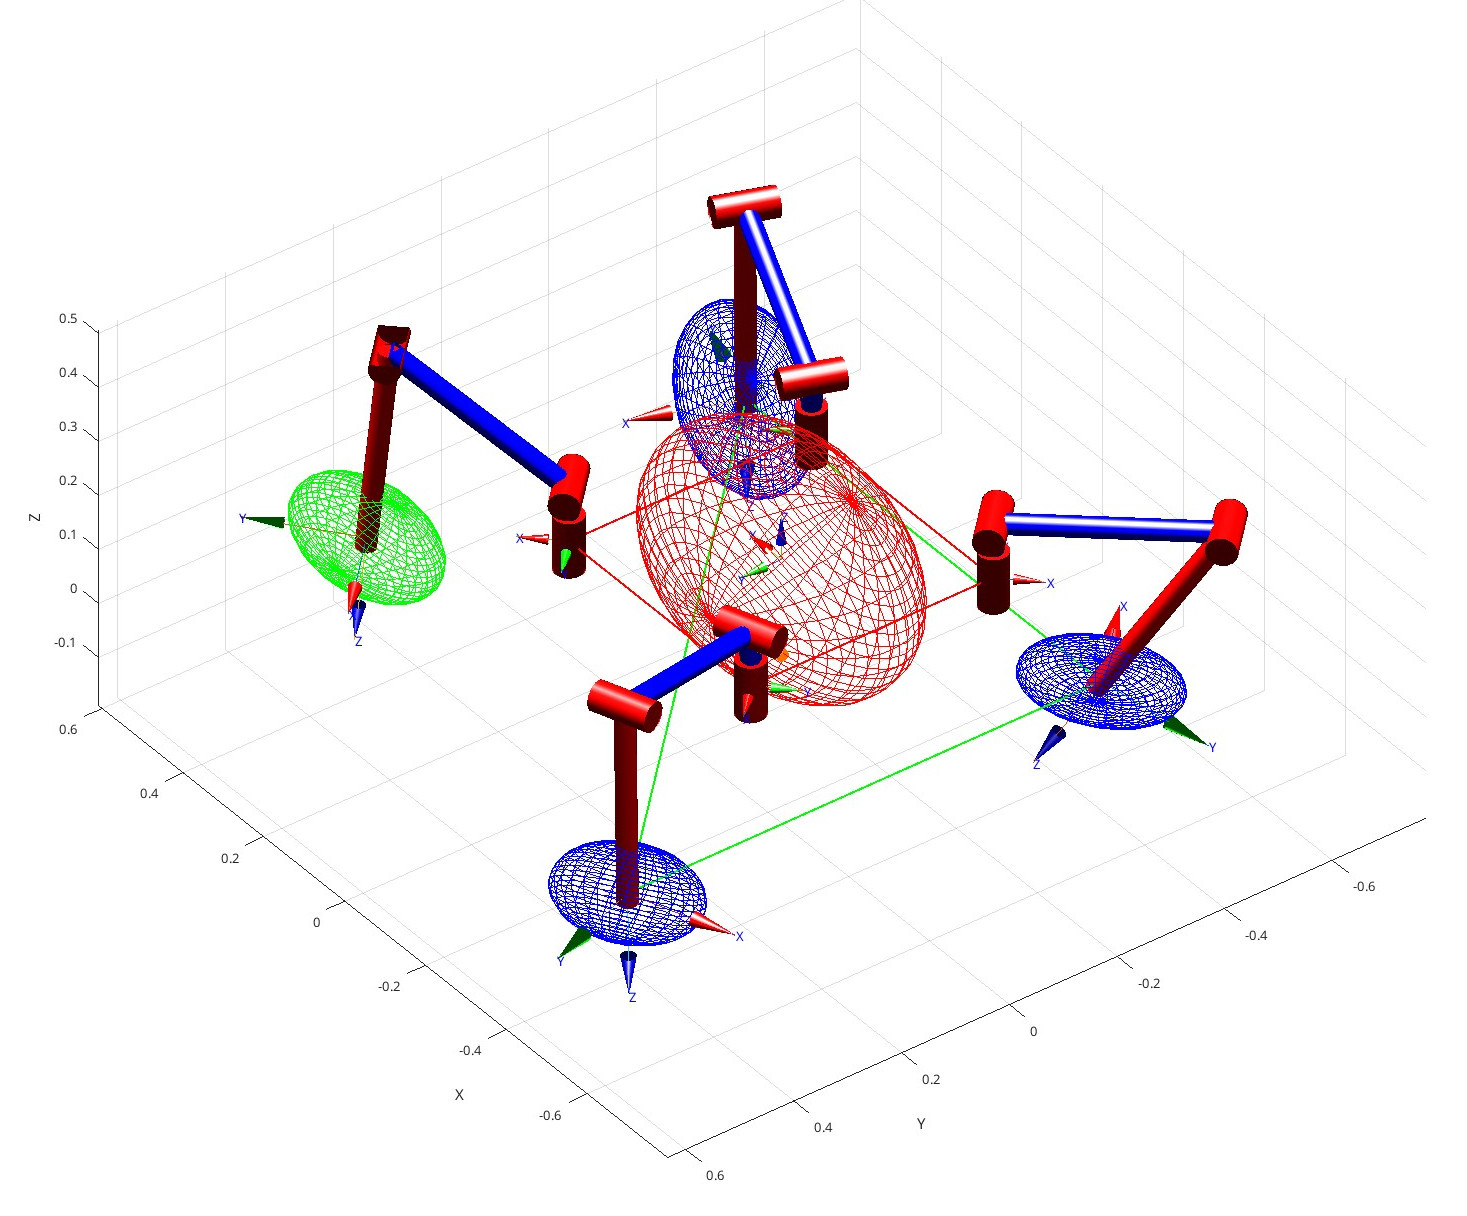
\includegraphics[width=0.35\textwidth]{Images/img_ch3/ex1_z01_xneg01_yneg01_LFup_ortho.jpg}}
    \subfloat[z=0.1, x=-0.1, y=-0.1, and LF up, xy view \label{fig:ex1_z01_xneg01_yneg01_LFup_xy}]{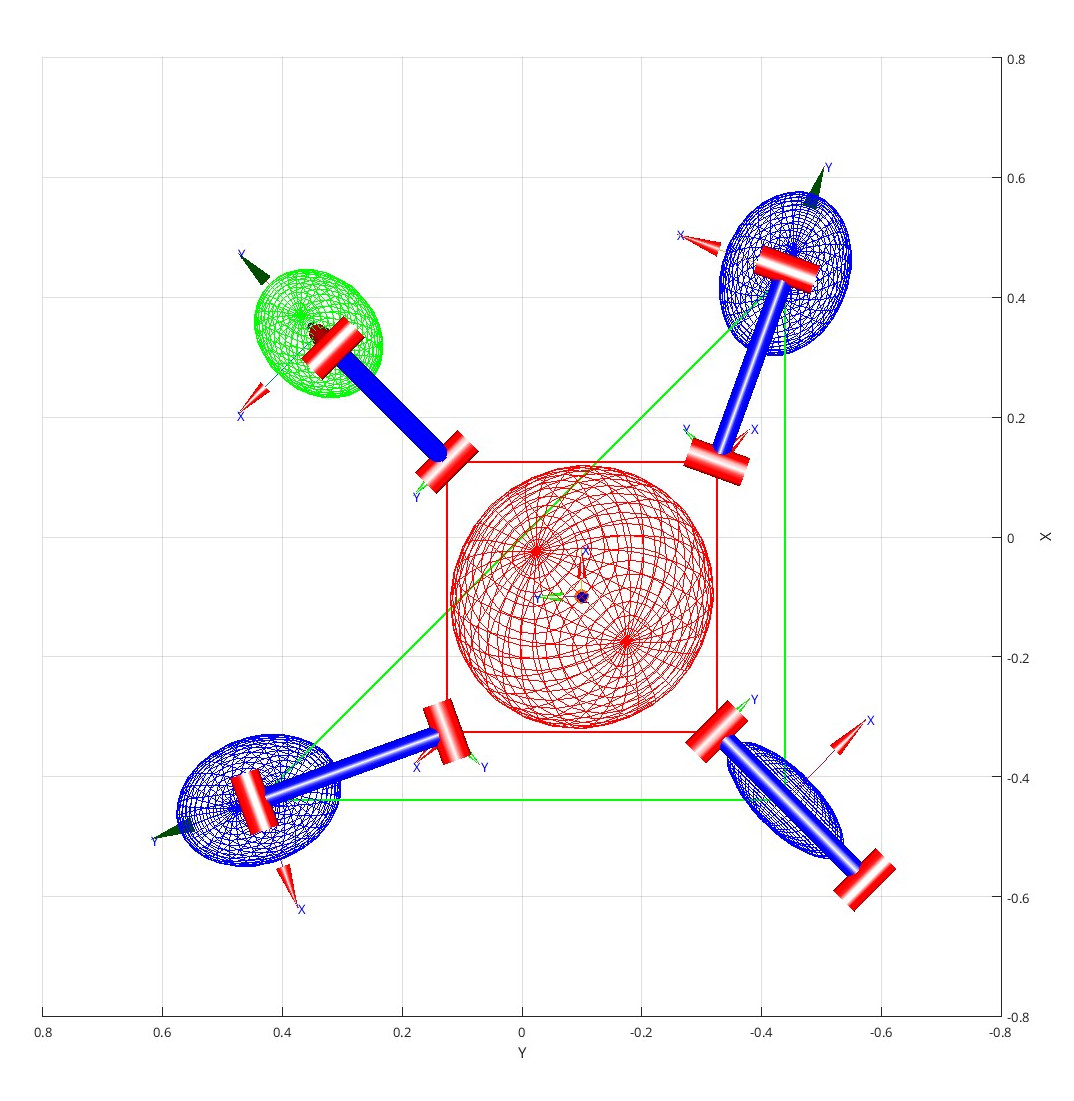
\includegraphics[width=0.35\textwidth]{Images/img_ch3/ex1_z01_xneg01_yneg01_LFup_xy.jpg}} 
    \caption[LimbedEx1 ME after LF limb up and base translation]{LimbedEx1 ME after LF limb up and base translation}
    \label{fig:ex1_rise_limb}
\end{figure}

\subsubsection{Example 2: Hexapod with 3-DOFs Limbs}
\label{sec:BME_hexapod}

This example is an extension of the previous one, to prove that more limbs are not a problem, therefore it is considered a 6-limbed robot with the same limb structure as before (now referred to as LimbedEx2). 
The robot is represented in Fig.\ref{fig:ex2_robot}, with all limbs in the zero configuration $\mathbf{q_0} = \begin{bmatrix}
    0 & 0 & 0
\end{bmatrix}^T$ and in the initial walking configuration $\mathbf{q_W} = \begin{bmatrix}
    0 & -\pi/6 & \frac{2}{3}\pi
\end{bmatrix}^T$.

\begin{figure}[H]
    \centering
    \subfloat[LimbedEx2 with limbs in $\mathbf{q_0}$\label{fig:ex2_q0}]{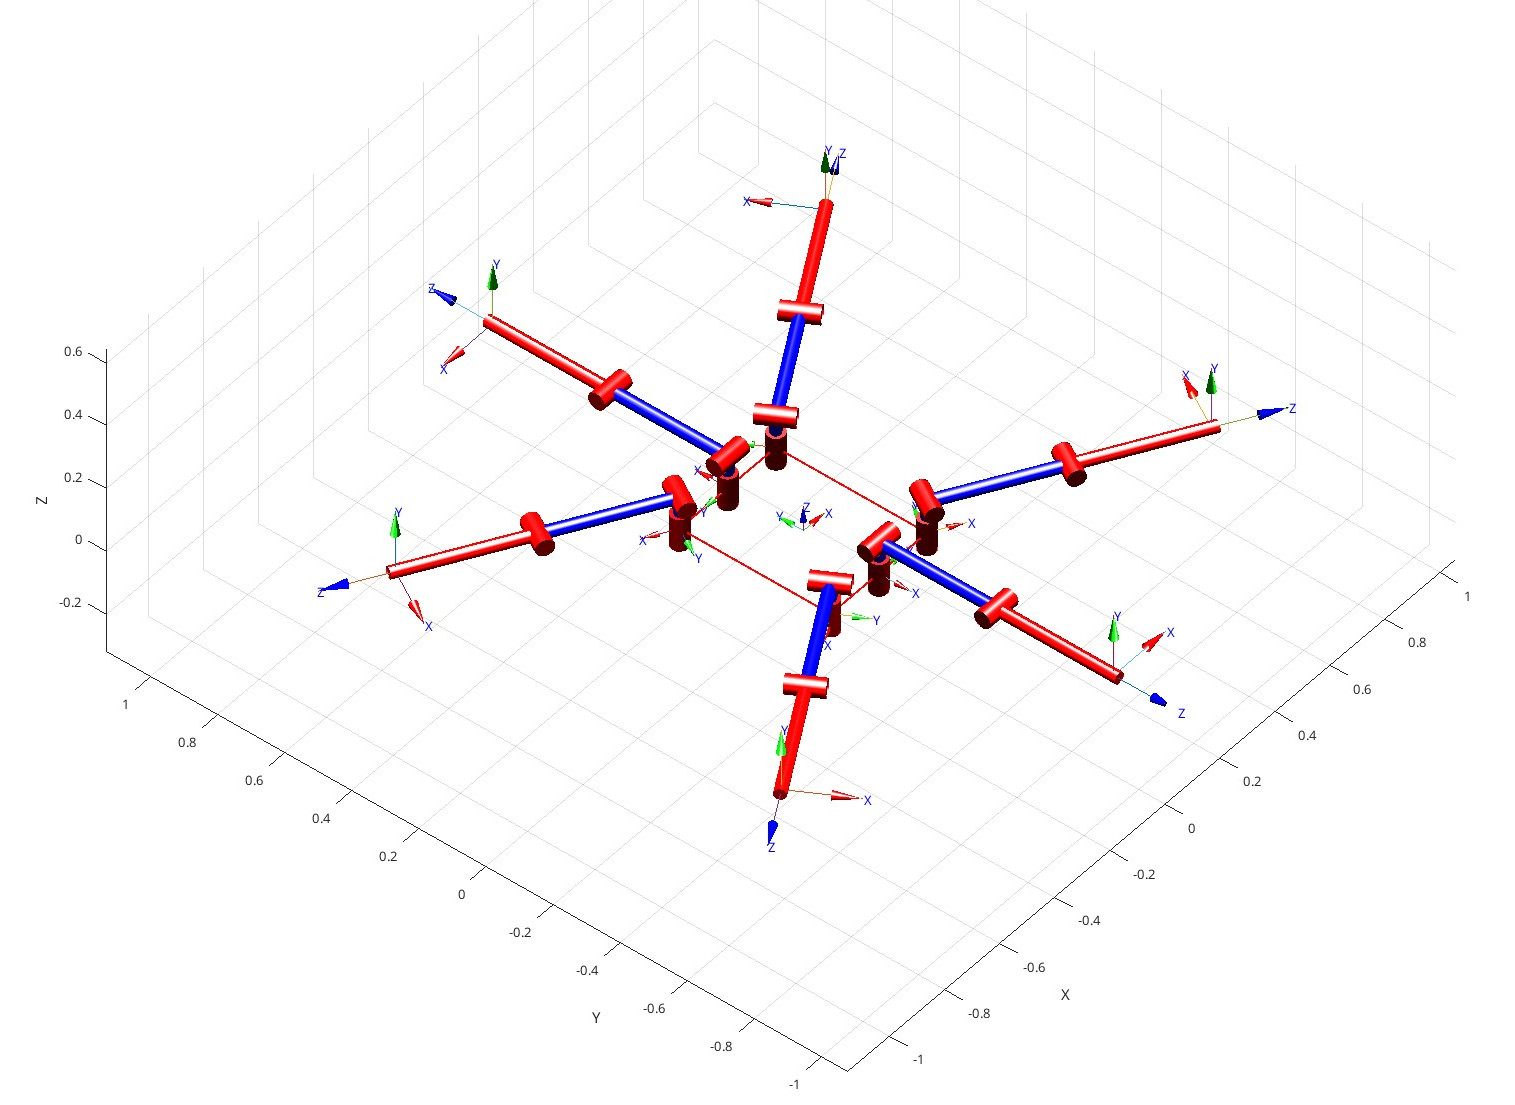
\includegraphics[width=0.45\textwidth]{Images/img_ch3/hexapod_q0.jpg}}
    \subfloat[LimbedEx2 with limbs in $\mathbf{q_W}$\label{fig:ex2_qw}]{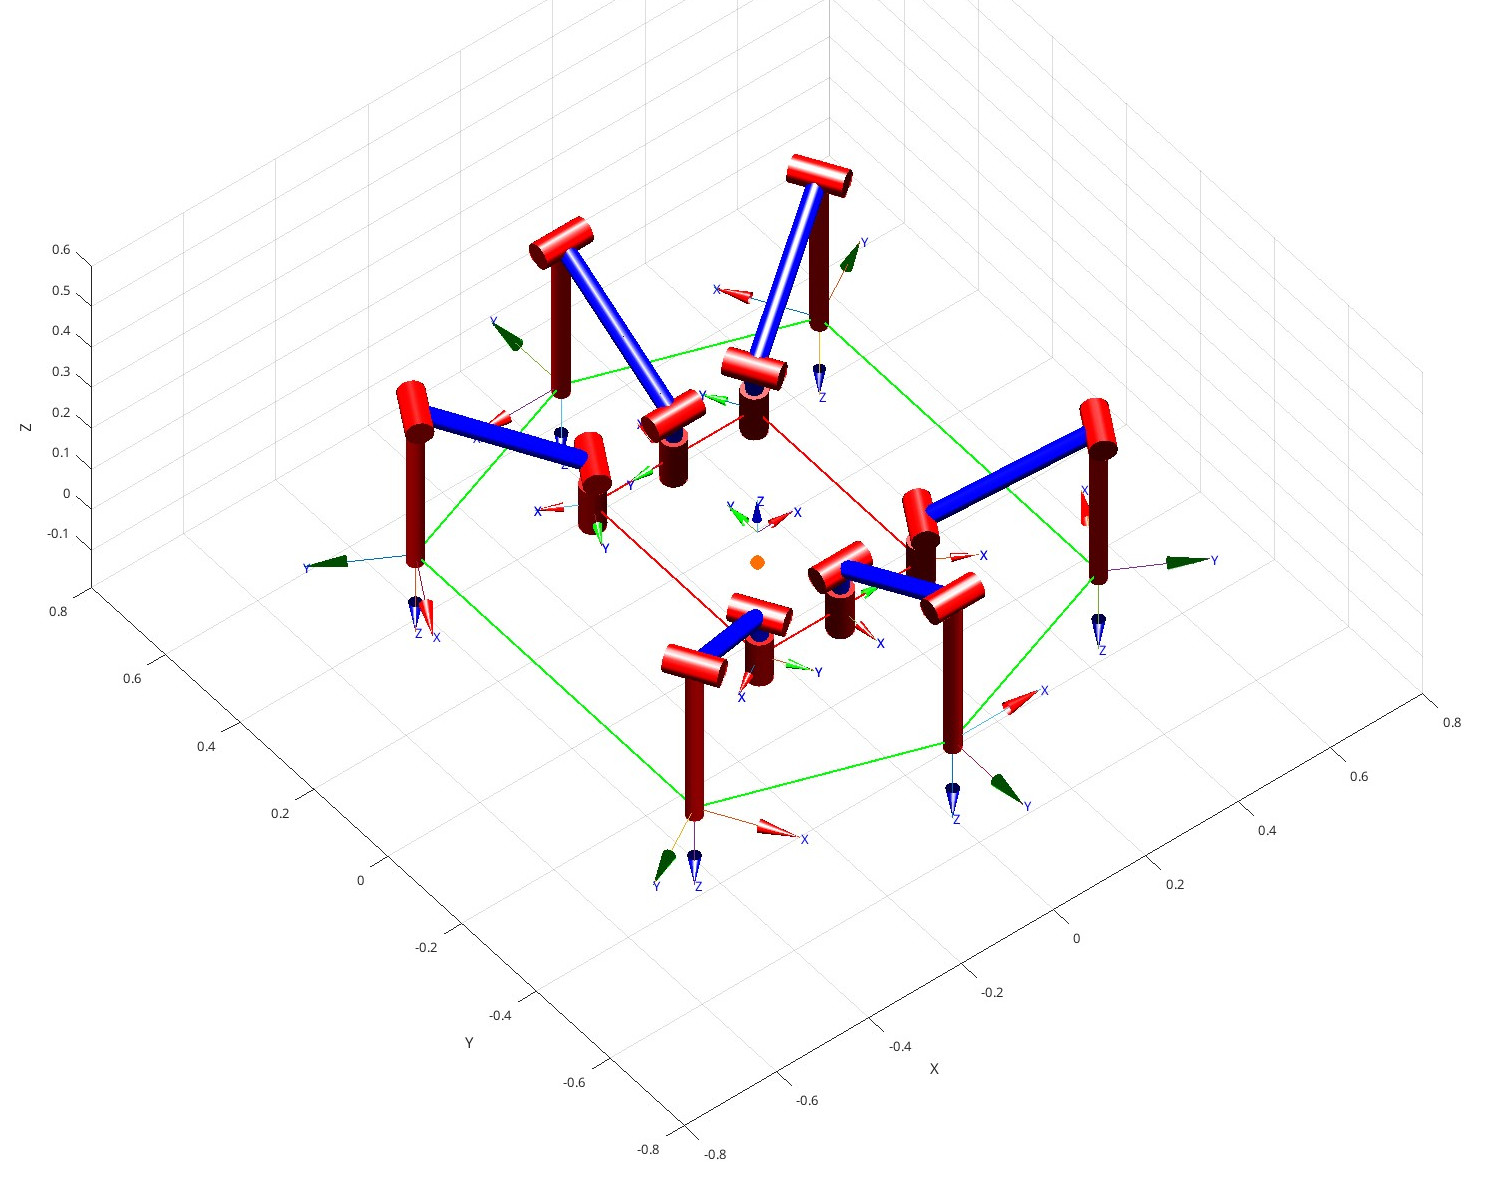
\includegraphics[width=0.45\textwidth]{Images/img_ch3/hexapod_qw.jpg}} 
    \caption[LimbedEx2 in zero and walking configuration]{LimbedEx2 in zero and walking configuration}
    \label{fig:ex2_robot}
\end{figure}

 Similarly to example 1, configurations computed as base motion from the walking one can be tested to evaluate the validity of the ATBVME for multi-limbed robots. The results obtained from the analysis of the ellipsoid shape and volume are the same as the previous example, with the same limitation in the unexpectedly increasing volume.  
 
\textbf{Walking Configuration}
\begin{figure}[H]
    \centering
    \subfloat[perspective view\label{fig:ex2_walking_ortho}]{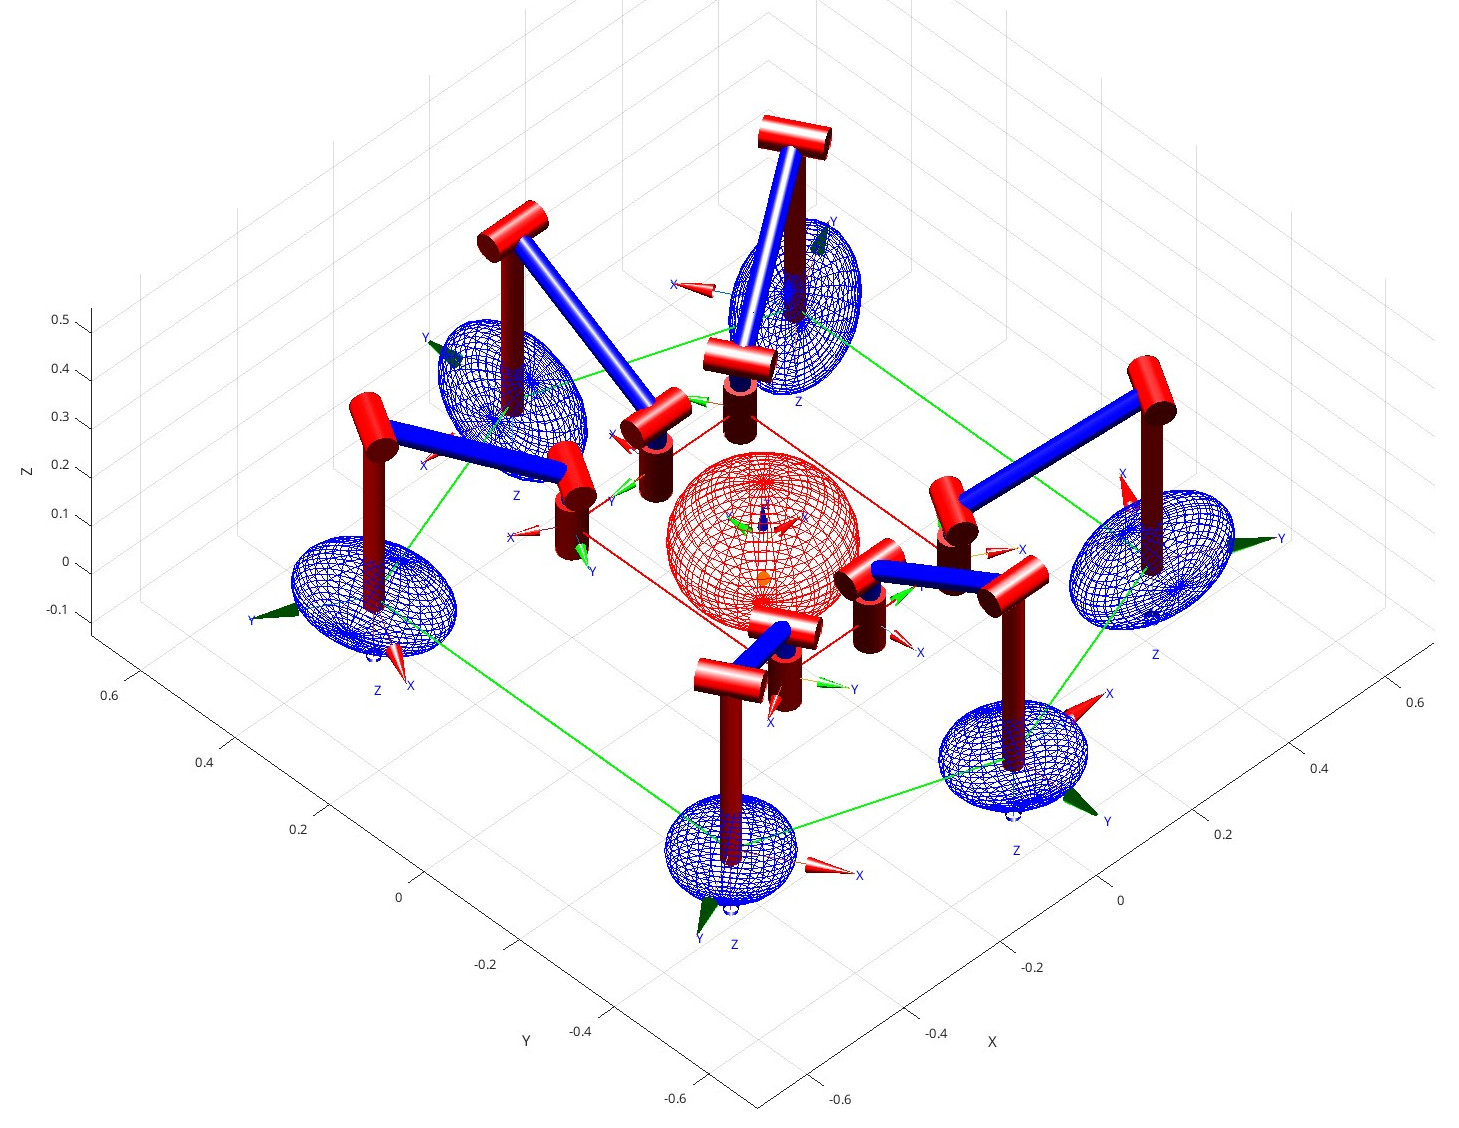
\includegraphics[width=0.3\textwidth]{Images/img_ch3/ex2_walking_ortho.jpg}}
    \subfloat[xy view\label{fig:ex2_walking_xy}]{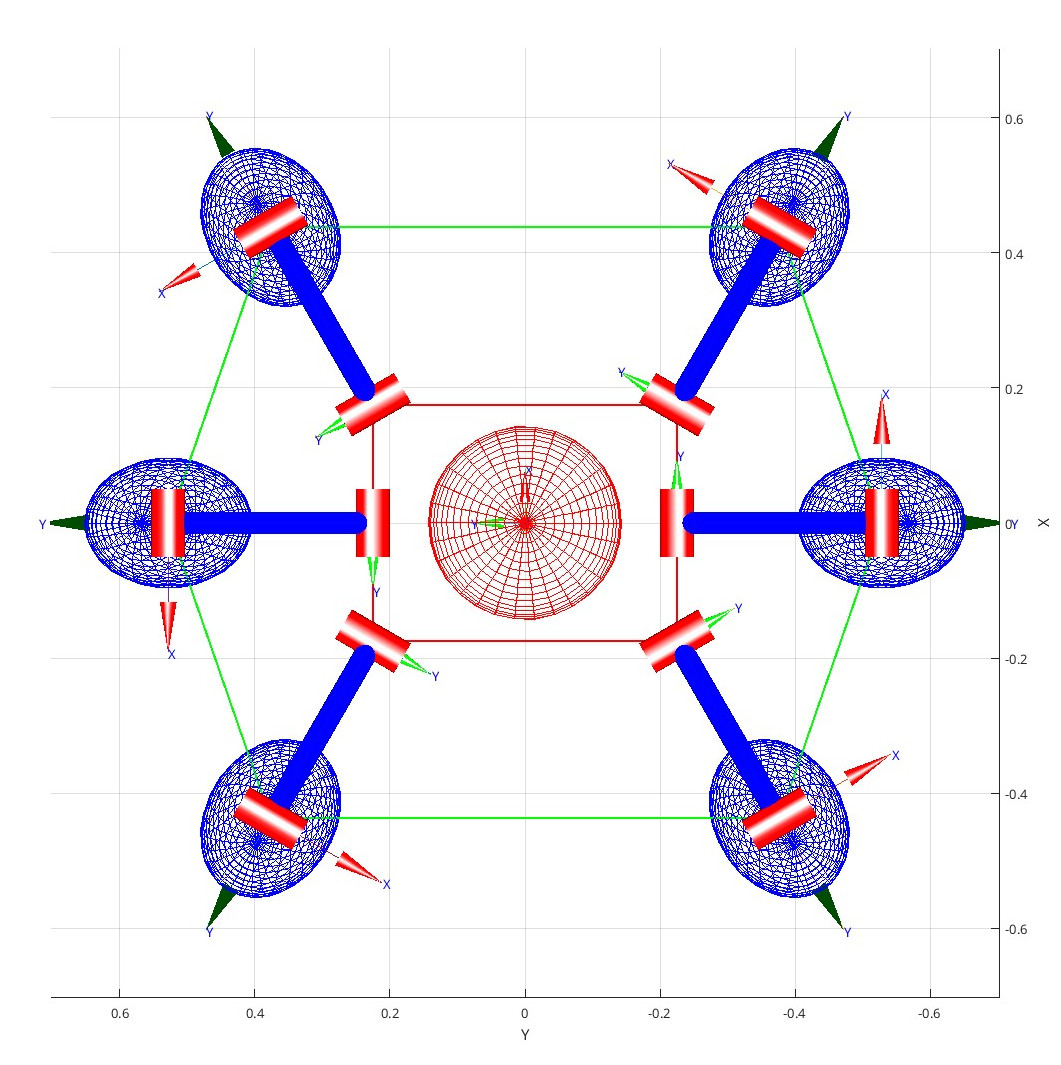
\includegraphics[width=0.3\textwidth]{Images/img_ch3/ex2_walking_xy.jpg}} 
    \subfloat[xz view\label{fig:ex2_walking_xz}]
    {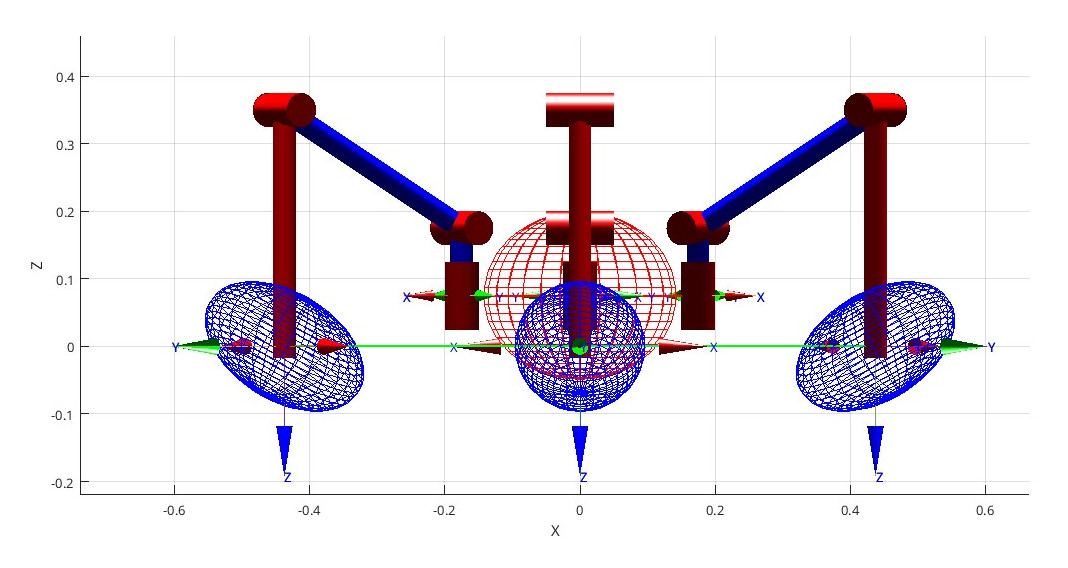
\includegraphics[width=0.3\textwidth]{Images/img_ch3/ex2_walking_xz.jpg}} 
    \caption[LimbedEx2 ME in walking configuration]{LimbedEx2 ME in walking configuration}
    \label{fig:ex2_walking}
\end{figure}
\newpage
\textbf{Base z translations}
\begin{figure}[H]
    \centering
    \subfloat[z=0.2, perspective view\label{fig:ex2_z020_xy}]{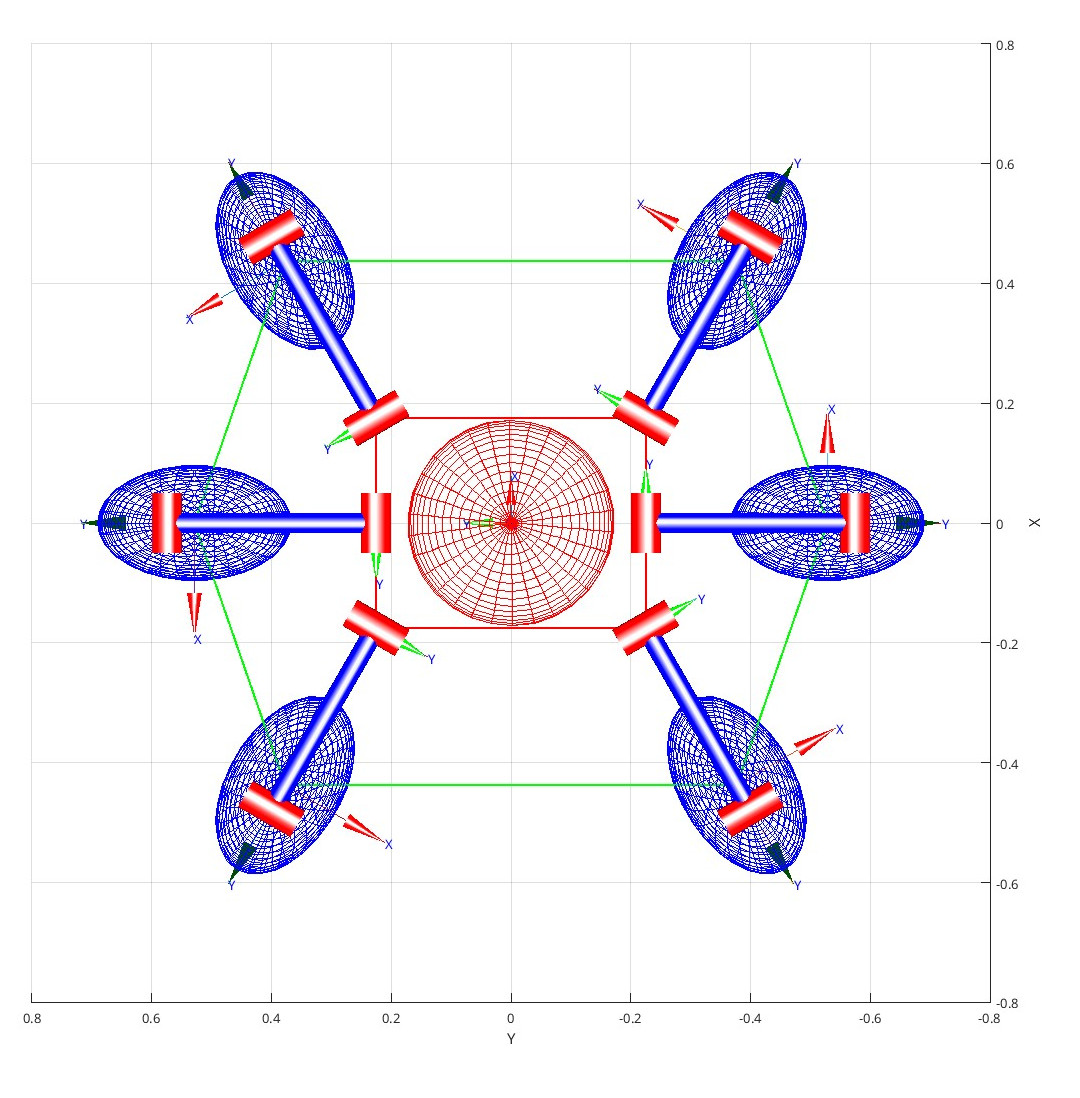
\includegraphics[width=0.35\textwidth]{Images/img_ch3/ex2_z020_xy.jpg}}
    \subfloat[z=0.2, xy view\label{fig:ex2_z020_xz}]{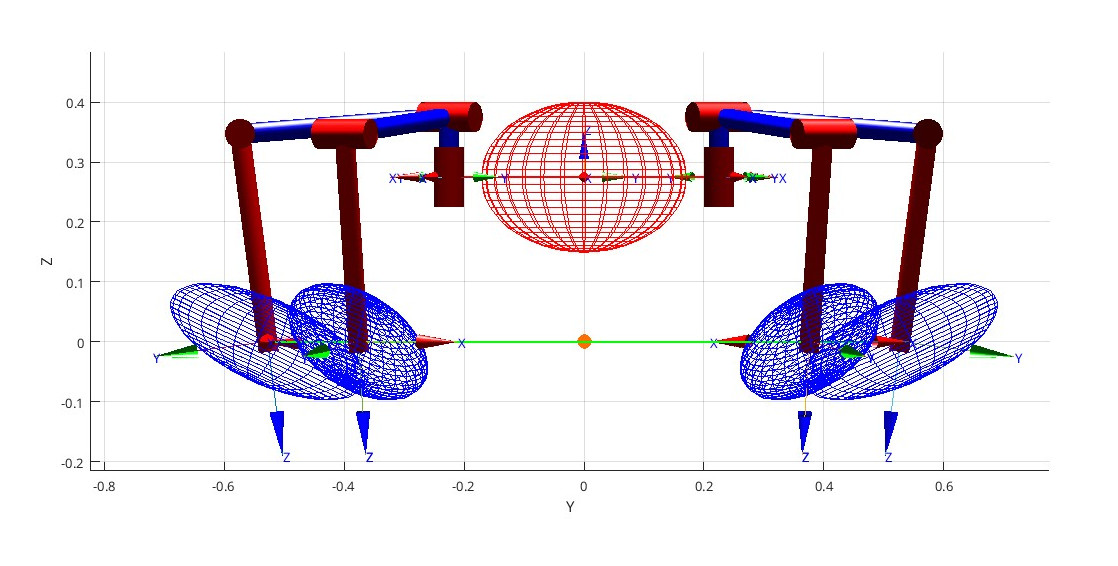
\includegraphics[width=0.35\textwidth]{Images/img_ch3/ex2_z020_xz.jpg}} \\
    \subfloat[z=0.4, xz view\label{fig:ex2_z040_xy}]
    {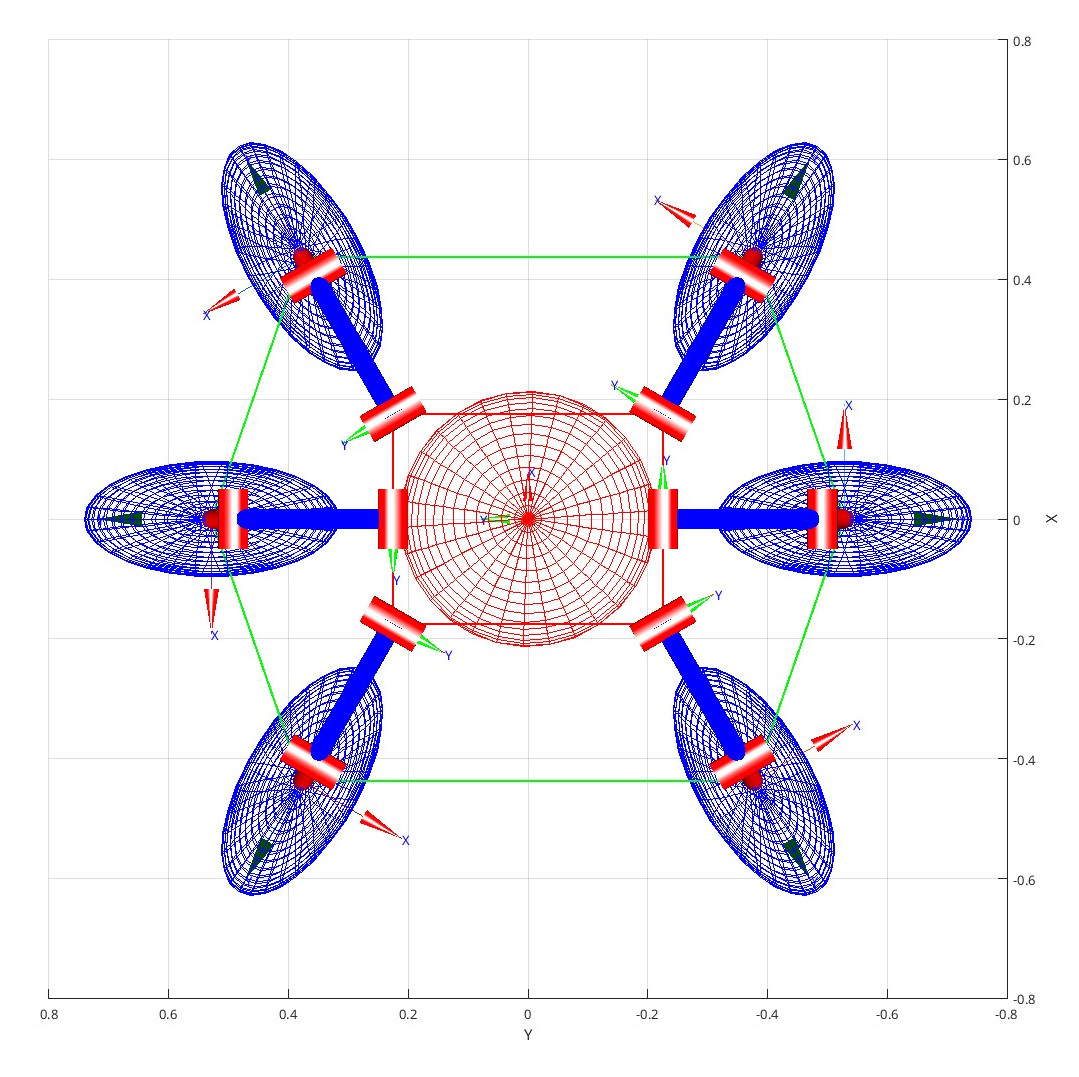
\includegraphics[width=0.35\textwidth]{Images/img_ch3/ex2_z040_xy.jpg}} 
    \subfloat[z=0.4, yz view\label{fig:ex2_z040_yz}]
    {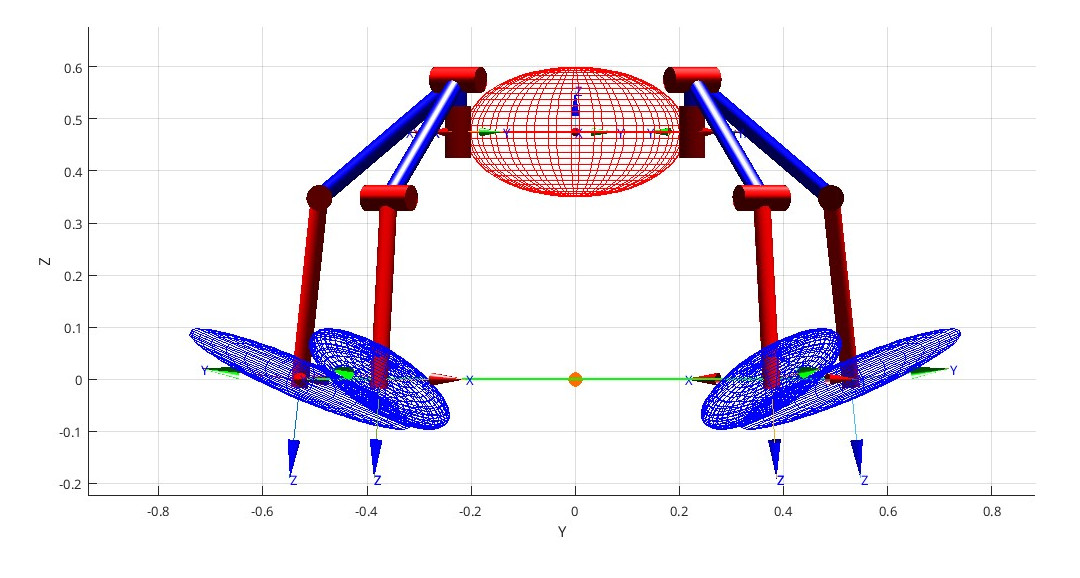
\includegraphics[width=0.35\textwidth]{Images/img_ch3/ex2_z040_yz.jpg}} 
    \caption[LimbedEx2 ME after z base translation]{LimbedEx2 ME after z base translation}
    \label{fig:ex2_z}
\end{figure}

\textbf{Base x,y,z translations}
\begin{figure}[H]
    \centering
    \subfloat[perspective view\label{fig:ex2_xneg02_y01_z015_ortho}]{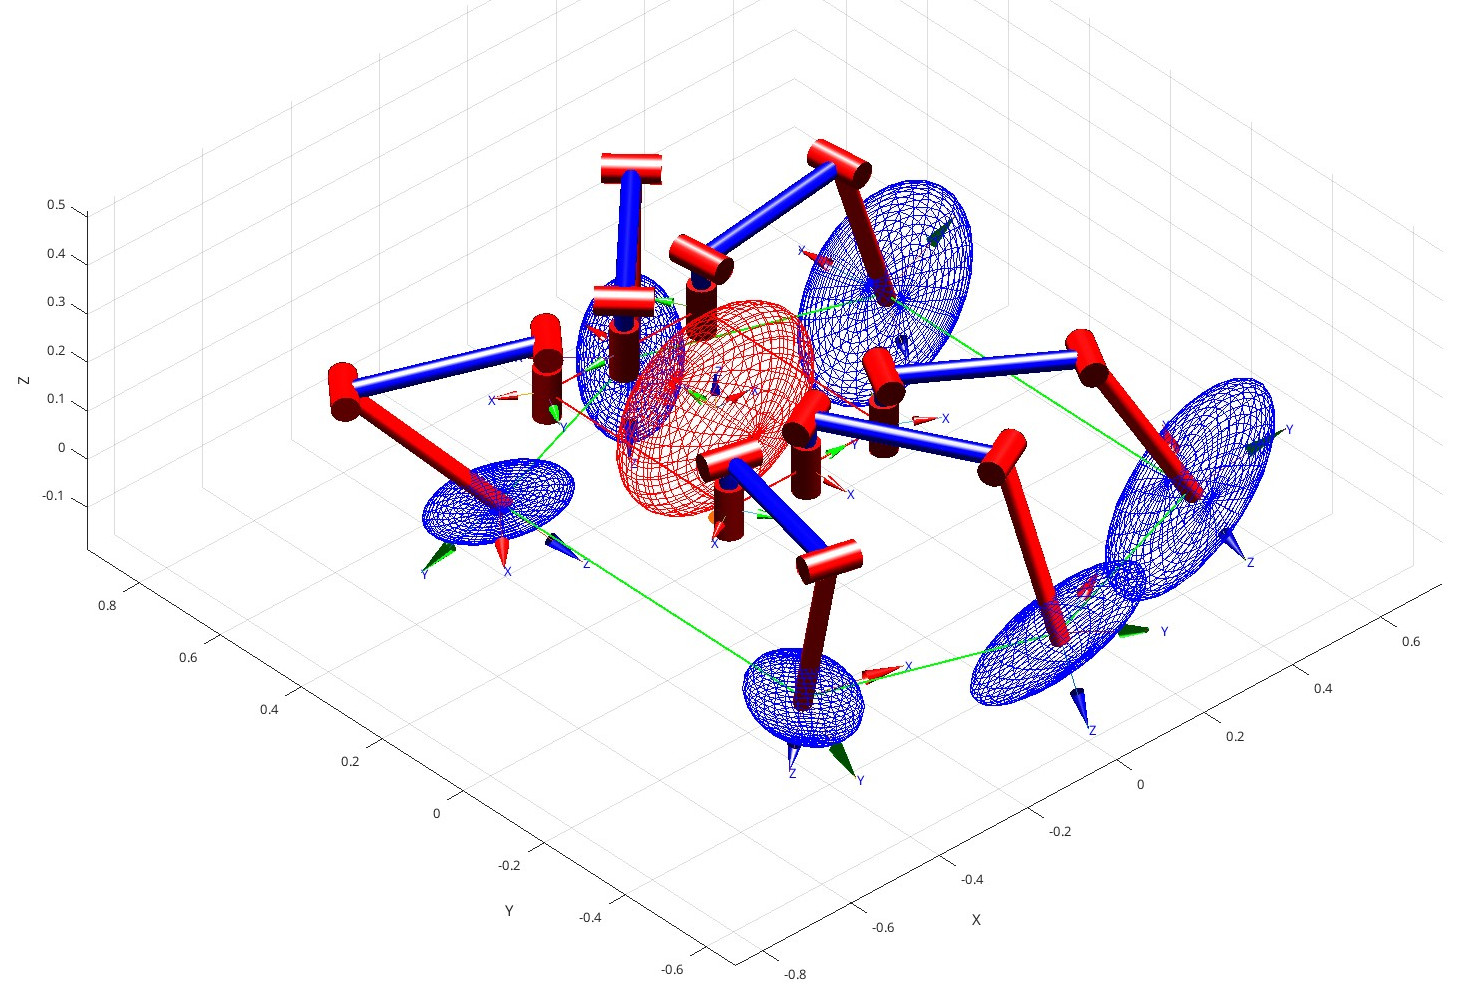
\includegraphics[width=0.3\textwidth]{Images/img_ch3/ex2_xneg02_y01_z015_ortho.jpg}}
    \subfloat[xy view\label{fig:ex2_xneg02_y01_z015_xy}]{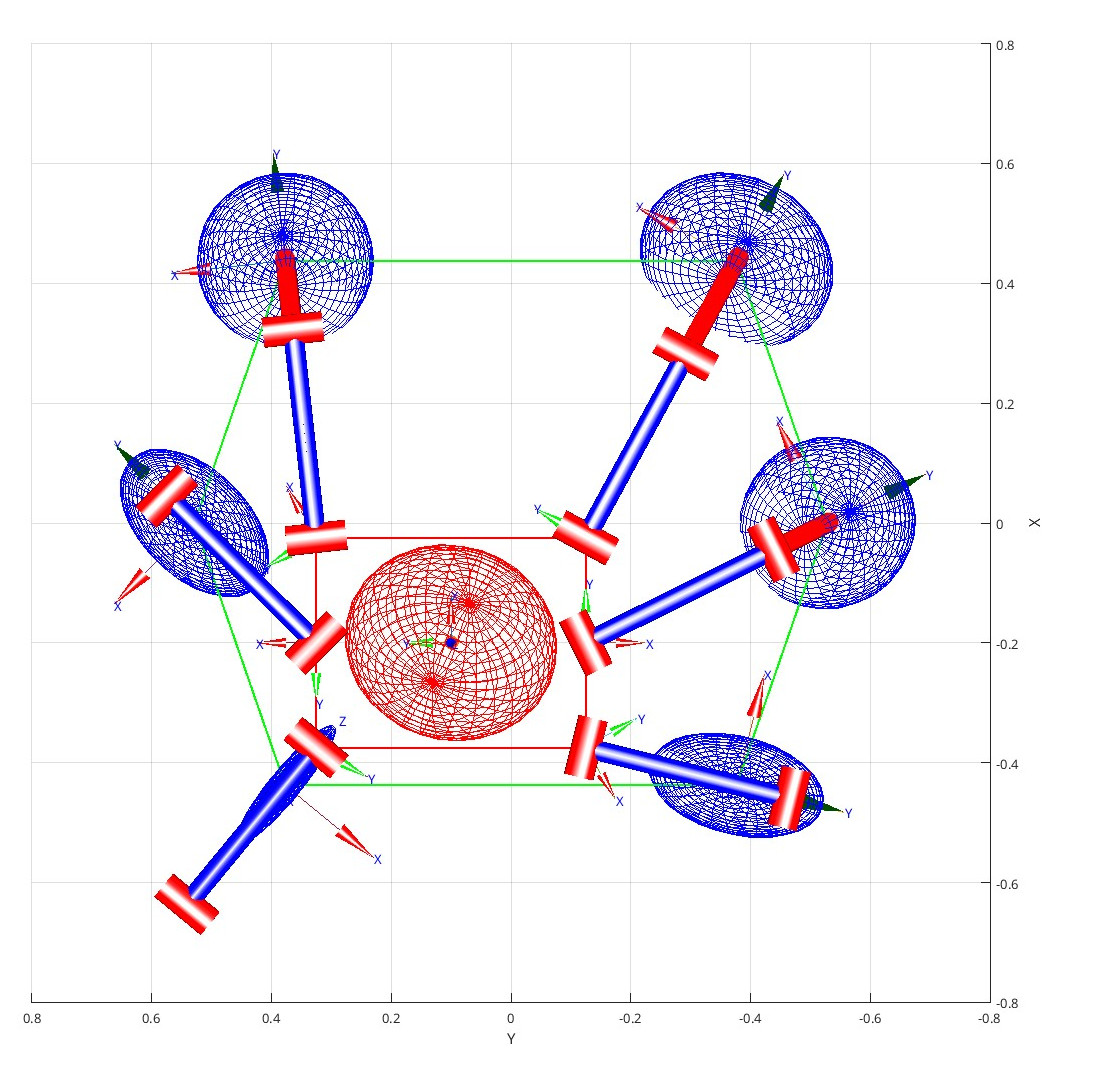
\includegraphics[width=0.3\textwidth]{Images/img_ch3/ex2_xneg02_y01_z015_xy.jpg}} 
    \subfloat[xz view\label{fig:ex2_xneg02_y01_z015_xz}]
    {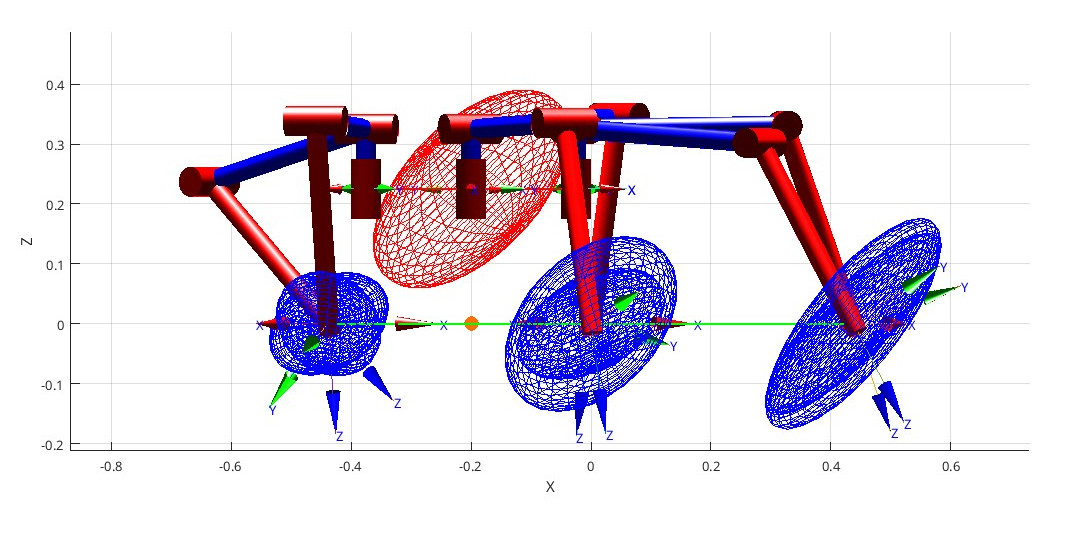
\includegraphics[width=0.3\textwidth]{Images/img_ch3/ex2_xneg02_y01_z015_xz.jpg}} 
    \caption[LimbedEx2 ME after base x=-0.2, y=0.1, z=0.15  translation]{LimbedEx2 ME after base x=-0.2, y=0.1, z=0.15  translation}
    \label{fig:ex2_xyz_translate}
\end{figure}
\newpage
\textbf{Raise Limb}
\begin{figure}[H]
    \centering
    \subfloat[LF and RF up, z=0.15, perspective view \label{fig:ex2_z015_LFRFUP_ortho}]{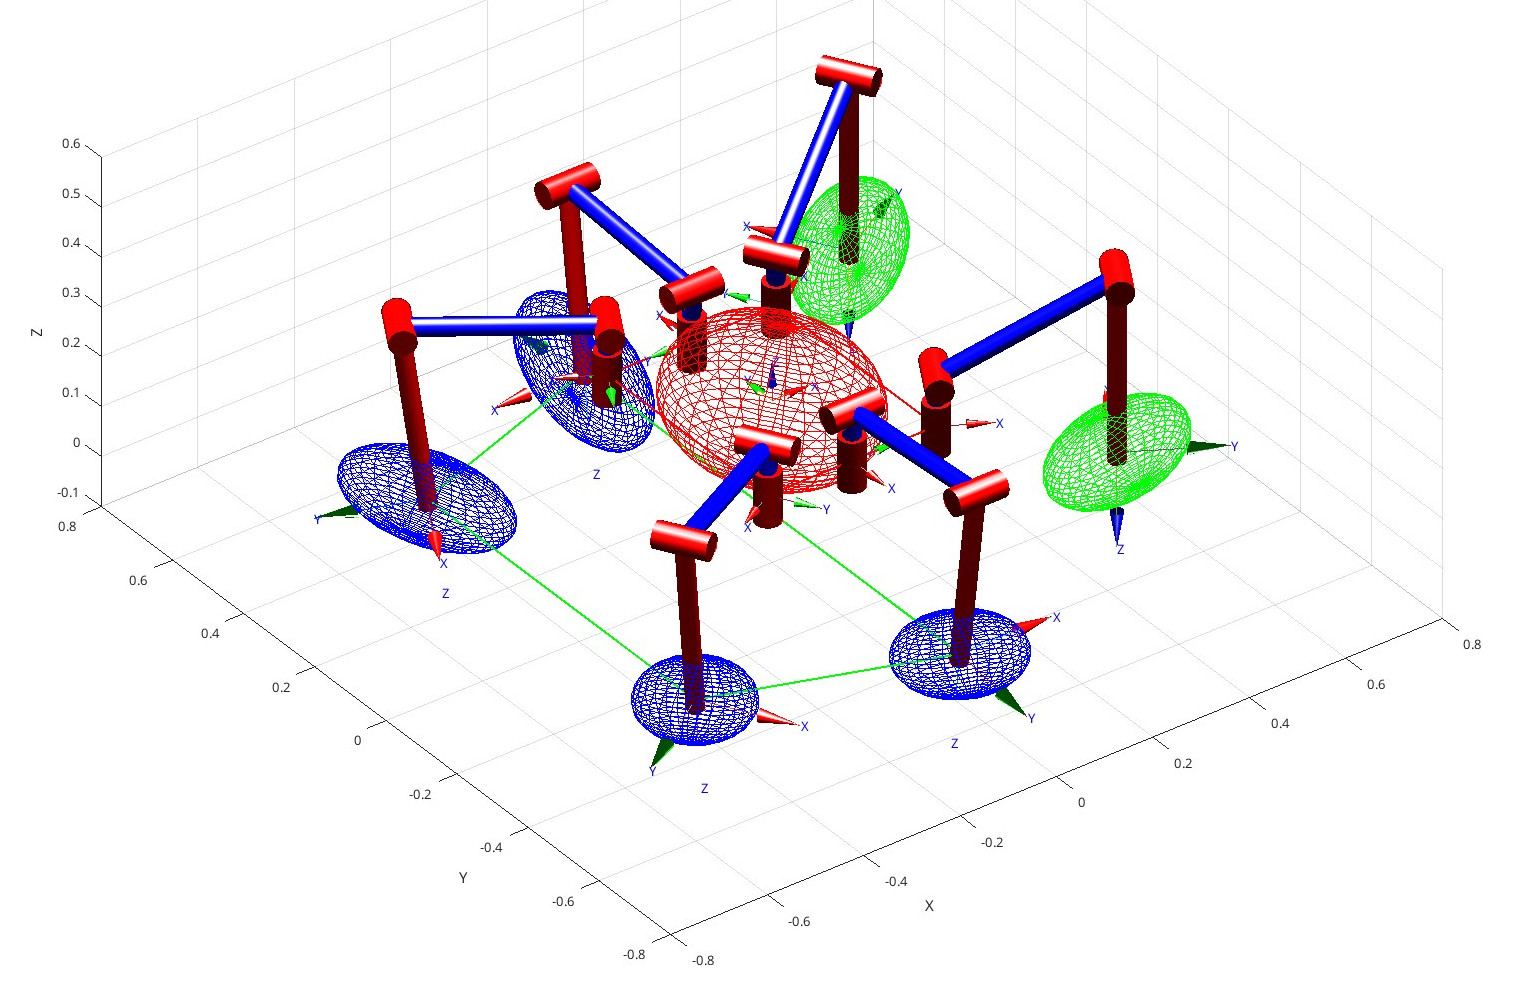
\includegraphics[width=0.45\textwidth]{Images/img_ch3/ex2_z015_LFRFUP_ortho.jpg}}
    \subfloat[LF and RF up, z=0.15,  xz view \label{fig:ex2_z015_LFRFUP_xz}]{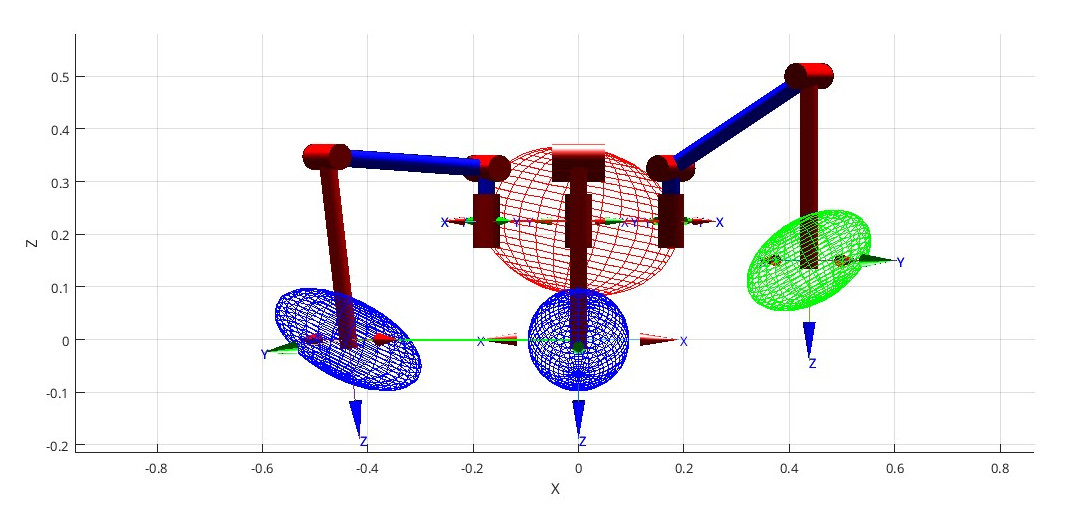
\includegraphics[width=0.45\textwidth]{Images/img_ch3/ex2_z015_LFRFUP_xz.jpg}} \\
    \subfloat[LF and RF up, z=0.15, x=-0.2, perspective view \label{fig:ex2_z015_xneg02_LFRFUP_ortho}]{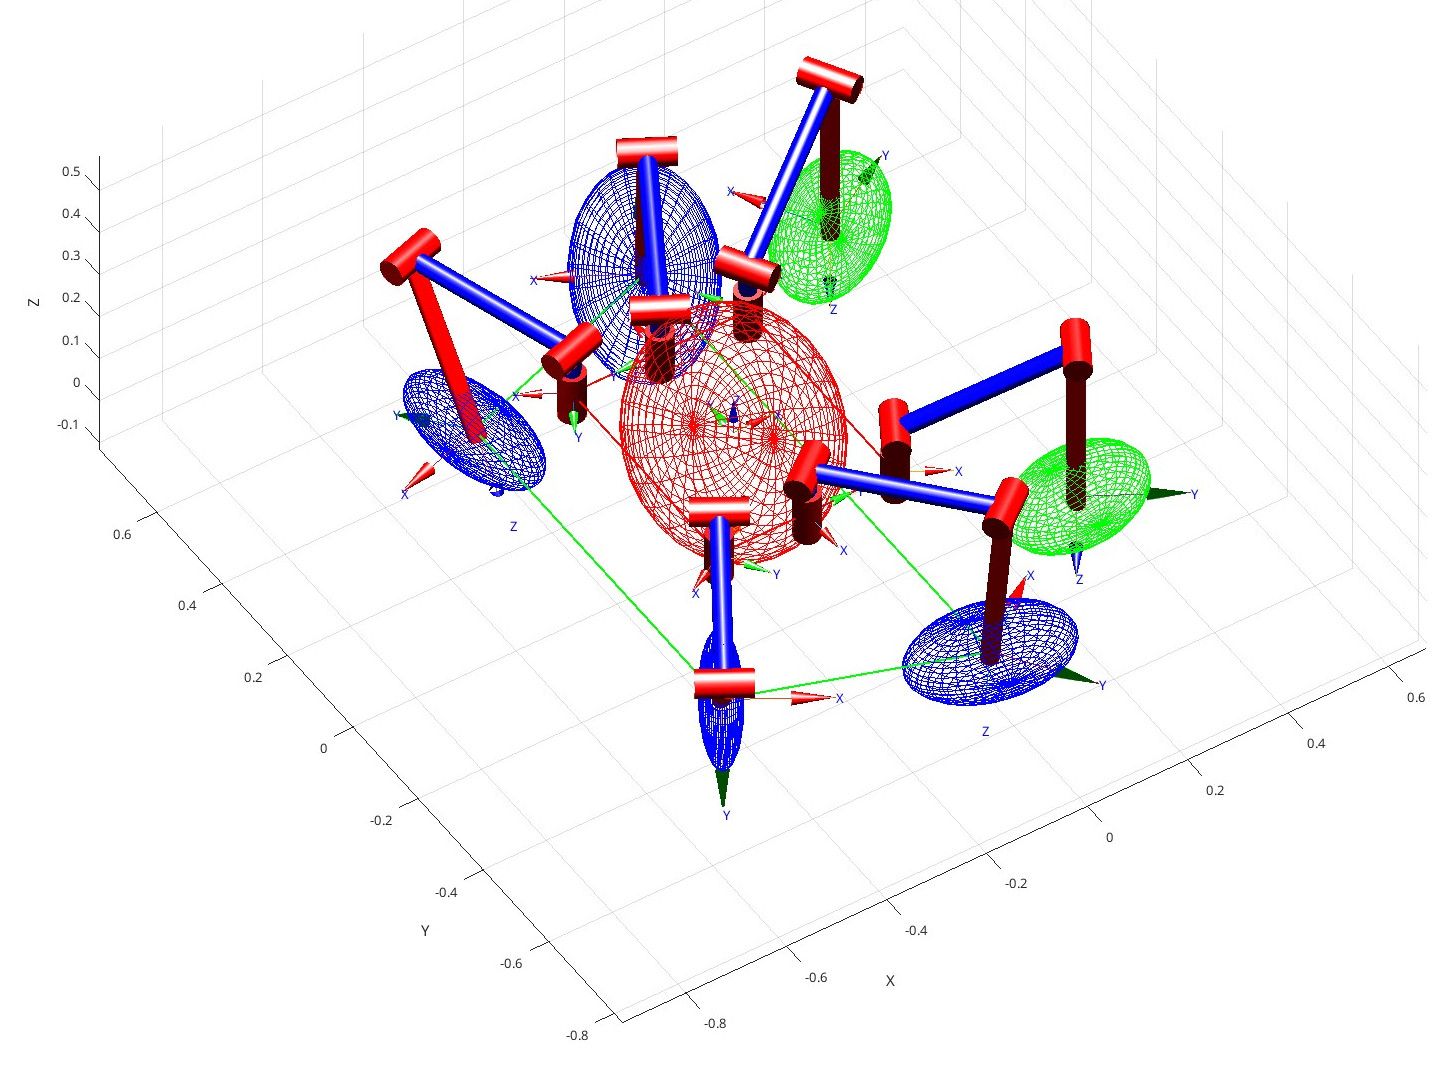
\includegraphics[width=0.45\textwidth]{Images/img_ch3/ex2_z015_xneg02_LFRFUP_ortho.jpg}}
    \subfloat[LF and RF up, z=0.15, x=-0.2, xz view \label{fig:ex2_z015_xneg02_LFRFUP_xz}]{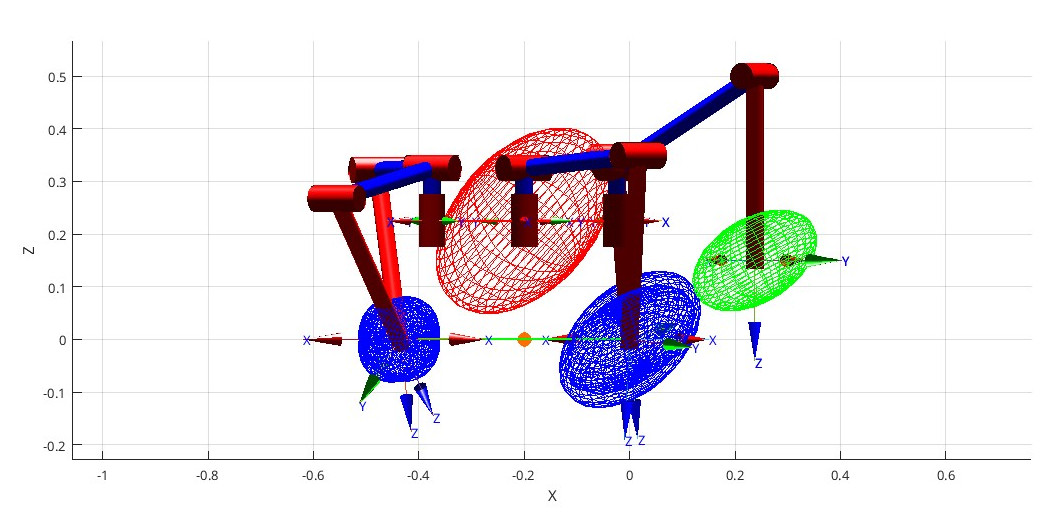
\includegraphics[width=0.45\textwidth]{Images/img_ch3/ex2_z015_xneg02_LFRFUP_xz.jpg}} \\
    \subfloat[LF, LB, RM up, z=0.15, perspective view \label{fig:ex2_z015_LFLBRMUP_ortho}]{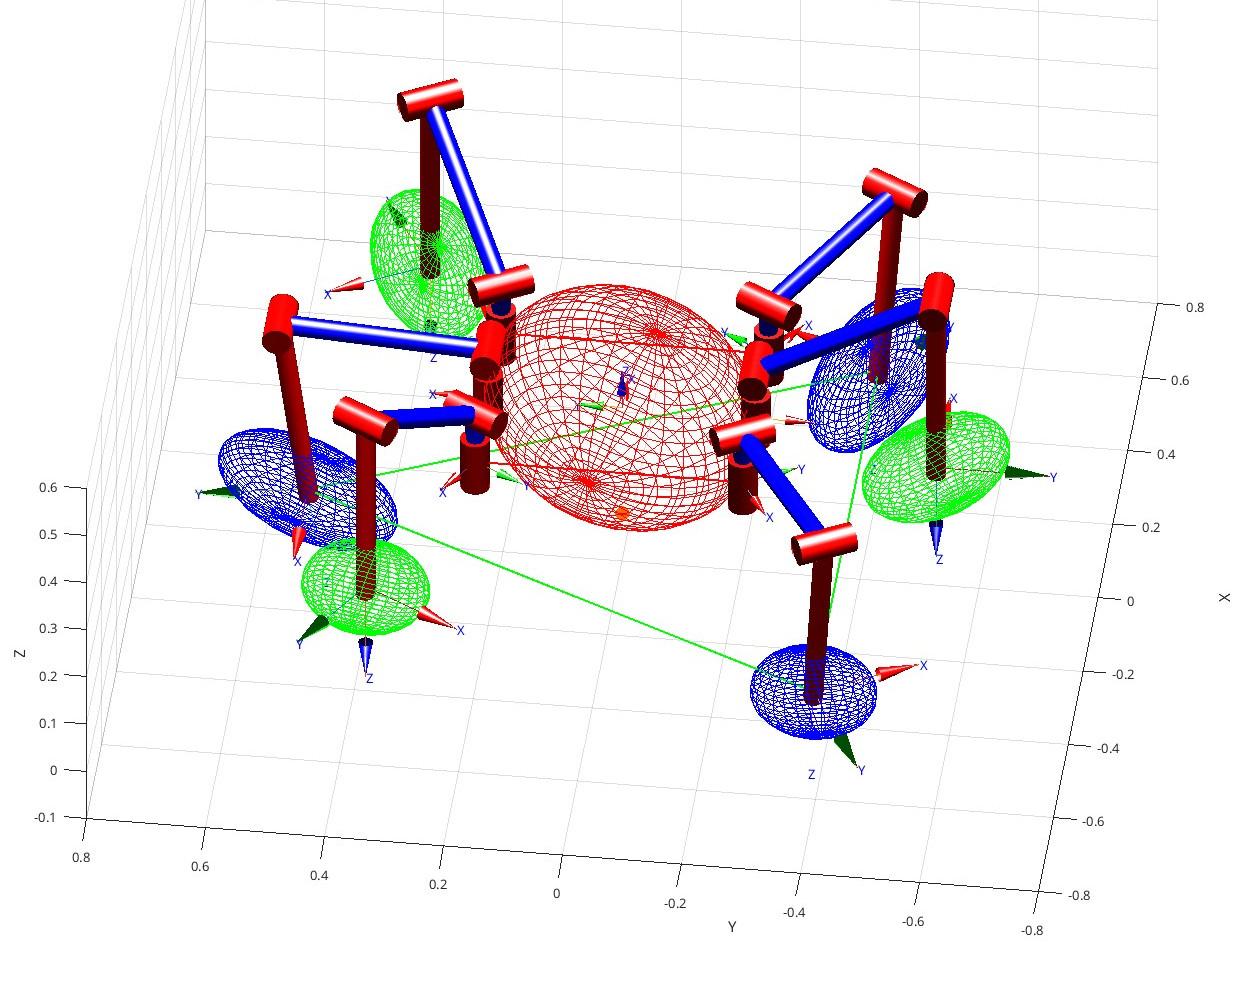
\includegraphics[width=0.45\textwidth]{Images/img_ch3/ex2_z015_LFLBRMUP_ortho.jpg}}
    \subfloat[LF, LB, RM up, z=0.15, yz view \label{fig:ex2_z015_LFLBRMUP_yz}]{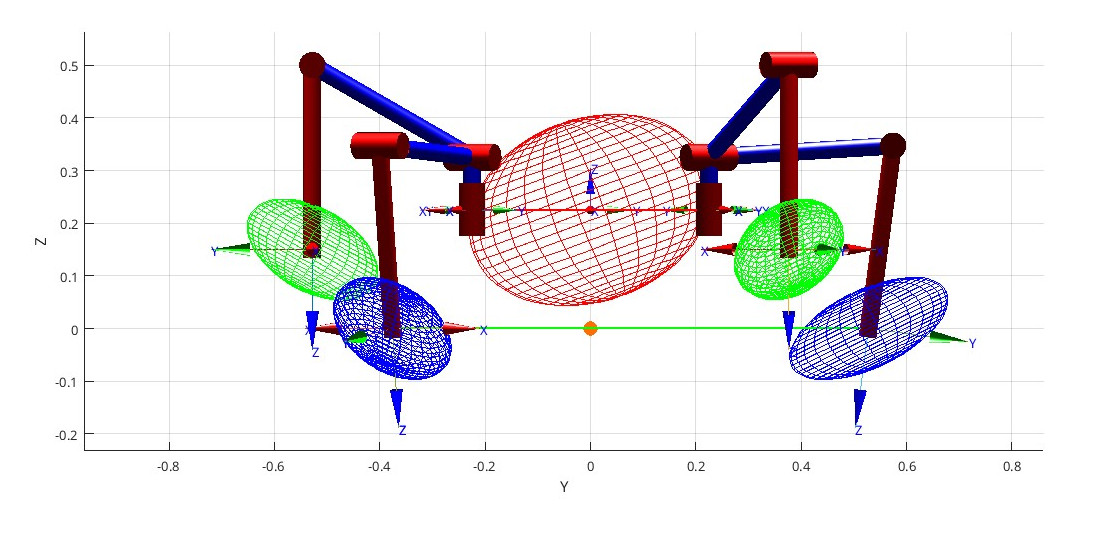
\includegraphics[width=0.45\textwidth]{Images/img_ch3/ex2_z015_LFLBRMUP_yz.jpg}}
    \caption[LimbedEx2 ME after limbs raise and base translation]{LimbedEx2 ME after limbs raise and base translation}
    \label{fig:ex2_rise_limb}
\end{figure}


\subsection{Biomechanics Examples, the Grasshopper}
\label{sec:ME_bio_inspired}

A final example is described in this section, in this case, a common approach to prove the validity of novel theory is used, and biomechanics is considered.

It is common practice to take inspiration from nature\cite{Biomimetics}, and walking robots themselves come from studies on animals' anatomy and gaits\cite{Todd}.
One of the fields of biological sciences is 
Biomechanics, which studies biological systems in their structures, functions, and working principles, and it provides useful insights for bio-inspired engineering solutions. 

It is possible to rely on biomechanical analysis in the opposite direction, proving that a mathematical theory is meaningful because it is coherent with nature. 

For example, applying the manipulability ellipsoid theory of T.Yoshikawa\cite{ManipulabilityYoshikawa} on a reduced human arm model, intuitive results can be found\cite{Siciliano}.

In the same way, here the BME theory is used to analyze the biomechanics of a grasshopper (as the one in Fig.\ref{fig:grasshopper_real}), and if the theory is meaningful results consistent with real documented behavior have to be found. 
The choice of this animal is motivated by its ability to jump, and the particular rear legs configuration taken in preparation for jumping, which inspired different robotic studies and actuation mechanism
\cite{Grasshopper1}\cite{Grasshopper2}\cite{Grasshopper3}.

\begin{figure}[H]
    \centering
    \subfloat[Grasshopper picture\label{fig:grasshopper_real}]{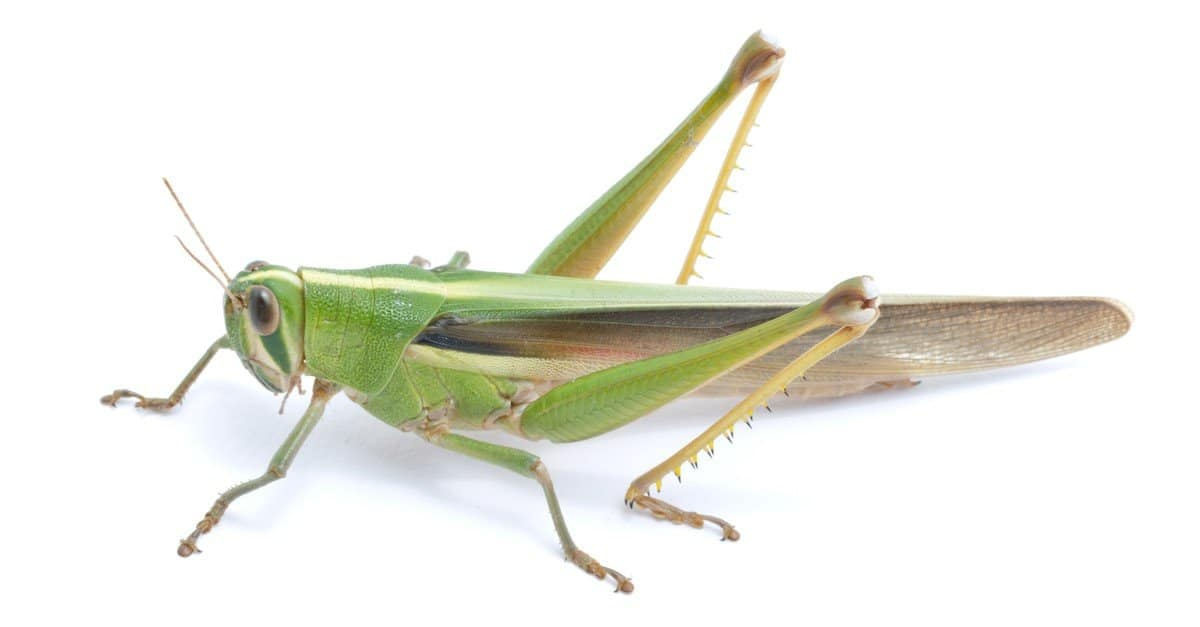
\includegraphics[width=0.4\textwidth]{Images/img_ch3/grasshopper_real.jpg}}\quad
    \subfloat[\cite{Grasshopper3}Anatomic scheme and measurements \label{fig:grasshopper_schema}]{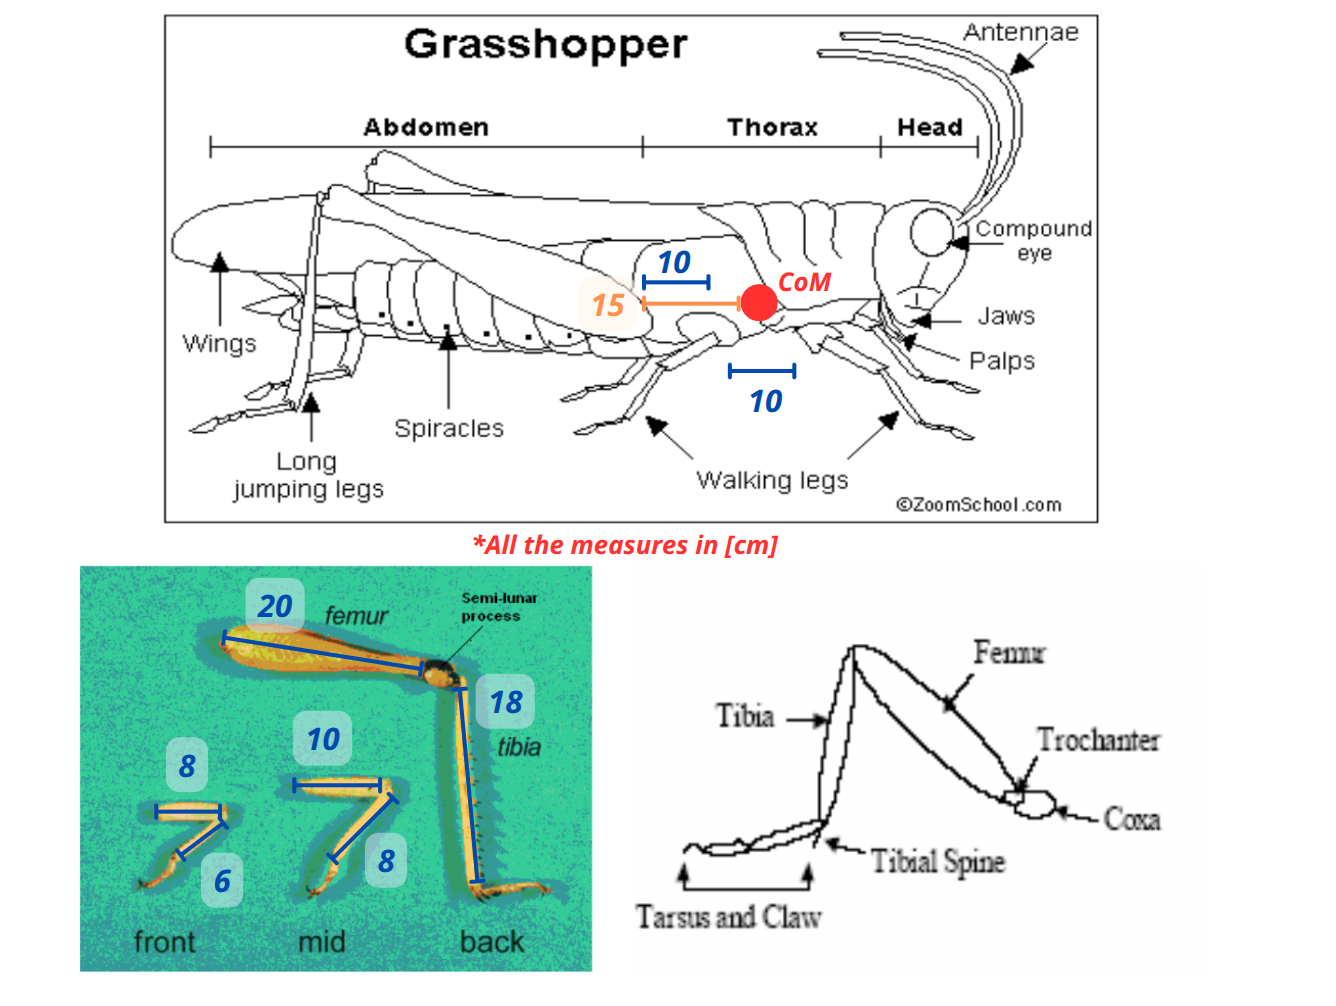
\includegraphics[width=0.55\textwidth]{Images/img_ch3/grasshopper_schema.png}} 
    \caption[Grasshopper picture and anatomic table]{Grasshopper picture and measurements}
    \label{fig:grasshopper}
\end{figure}

The jump is characterized by a big instantaneous body velocity when releasing the rear legs (due to particular leg anatomical features). 
If the BME works, in the jumping configuration the ATBVME should be oriented and elongated in the direction of the jump. 

Furthermore, if one of the rear legs is considered unusable, the jumping direction is affected, and if both cannot be used, the jumping ability is lost.
Finally, uncommon hind leg configurations and unrealistic body CoM locations are tested, to verify the consequence. 

First, an approximated kinematic model of the relevant DOFs of the legs (front, mid, and back) is derived.
The "approximation" neglects the additional links and joints used by the animal for additional mobility, not fundamental in the current analysis. 
The used dimensions of all leg links\cite{Grasshopper3} and the distance between them are reported in Fig.\ref{fig:grasshopper_schema}.

The model used for the legs is again the anthropomorphic arm, as the one in figure \ref{fig:antropomorphicDH} of the previous example. With this model, it is possible to represent the relevant joint and frames for this analysis. 
the DH parameters of all the legs models are reported in Tab.\ref{table:grasshopper_DH}.

\begin{table}[H]
\centering 
    \caption{Grasshopper legs DH parameters}
    \begin{tabular}{ c }
    \textbf{Front Legs parameters}
    \end{tabular}
    \begin{tabular}{| c | c | c | c | c | c |}
    \hline
    \rowcolor{bluepoli!40}
%    \rowcolor{bluepoli!40}
     \textbf{Link} &  $a_i$ $[m]$ & $\alpha_i$ $[rad]$ & $d_i$ $[m] $ & $\theta_i$ $[rad]$ & $\theta_{offset, i}$ $[rad]$ \T\B \\
    \hline \hline
    \textbf{CoxaF} ($i=1$) & 0.0 & $-\frac{\pi}{2}$ & 0.0  & $q_{F1}$  & 0.0 \T\B\\
    \hline 
    \textbf{FemurF} ($i=2$) & 0.08 & 0.0  & 0.0  & $q_{F2}$  & 0.0  \T\B\\
    \hline
    \textbf{TibiaF} ($i=3$) & 0.06  & 0.0  & 0.0  & $q_{F3}$ & 0.0 \T\B\\
    \hline
    \end{tabular}
    \begin{tabular}{ c }
    \\
    \textbf{Mid Legs parameters}
    \end{tabular}
    \begin{tabular}{| c | c | c | c | c | c |}
    \hline
    \rowcolor{bluepoli!40}
%    \rowcolor{bluepoli!40}
     \textbf{Link} &  $a_i$ $[m]$ & $\alpha_i$ $[rad]$ & $d_i$ $[m] $ & $\theta_i$ $[rad]$ & $\theta_{offset, i}$ $[rad]$ \T\B \\
    \hline \hline
    \textbf{CoxaM} ($i=1$) & 0.0 & $-\frac{\pi}{2}$ & 0.0  & $q_{M1}$  & 0.0 \T\B\\
    \hline 
    \textbf{FemurM} ($i=2$) & 0.10 & 0.0  & 0.0  & $q_{M2}$  & 0.0  \T\B\\
    \hline
    \textbf{TibiaM} ($i=3$) & 0.08  & 0.0  & 0.0  & $q_{M3}$ & 0.0 \T\B\\
    \hline
    \end{tabular} 
    \begin{tabular}{ c }
    \\
    \textbf{Back Legs parameters}
    \end{tabular}
    \begin{tabular}{| c | c | c | c | c | c |}
    \hline
    \rowcolor{bluepoli!40}
%    \rowcolor{bluepoli!40}
     \textbf{Link} &  $a_i$ $[m]$ & $\alpha_i$ $[rad]$ & $d_i$ $[m] $ & $\theta_i$ $[rad]$ & $\theta_{offset, i}$ $[rad]$ \T\B \\
    \hline \hline
    \textbf{CoxaB} ($i=1$) & 0.0 & $-\frac{\pi}{2}$ & 0.0  & $q_{B1}$  & 0.0 \T\B\\
    \hline 
    \textbf{FemurB} ($i=2$) & 0.20 & 0.0  & 0.0  & $q_{B2}$  & 0.0  \T\B\\
    \hline
    \textbf{TibiaB} ($i=3$) & 0.18  & 0.0  & 0.0  & $q_{B3}$ & 0.0 \T\B\\
    \hline
    \end{tabular} 
    \label{table:grasshopper_DH}
\end{table}

Figure \ref{fig:grasshopper_model} represents the overall kinematic model used in the following analysis, with the legs positioned using the distances reported in Fig.\ref{fig:grasshopper_schema}, and the initial legs orientation around the z-axis (Left Front (LF), Left Mid (LM), Left Back (LB)) is $\gamma_{LF} = \pi/6, \gamma_{LM} = \frac{2}{3}\pi, \gamma_{RB}=\pi$, and symmetric for the right ones: RF, RM, and RB.


\begin{figure}[H]
    \centering
    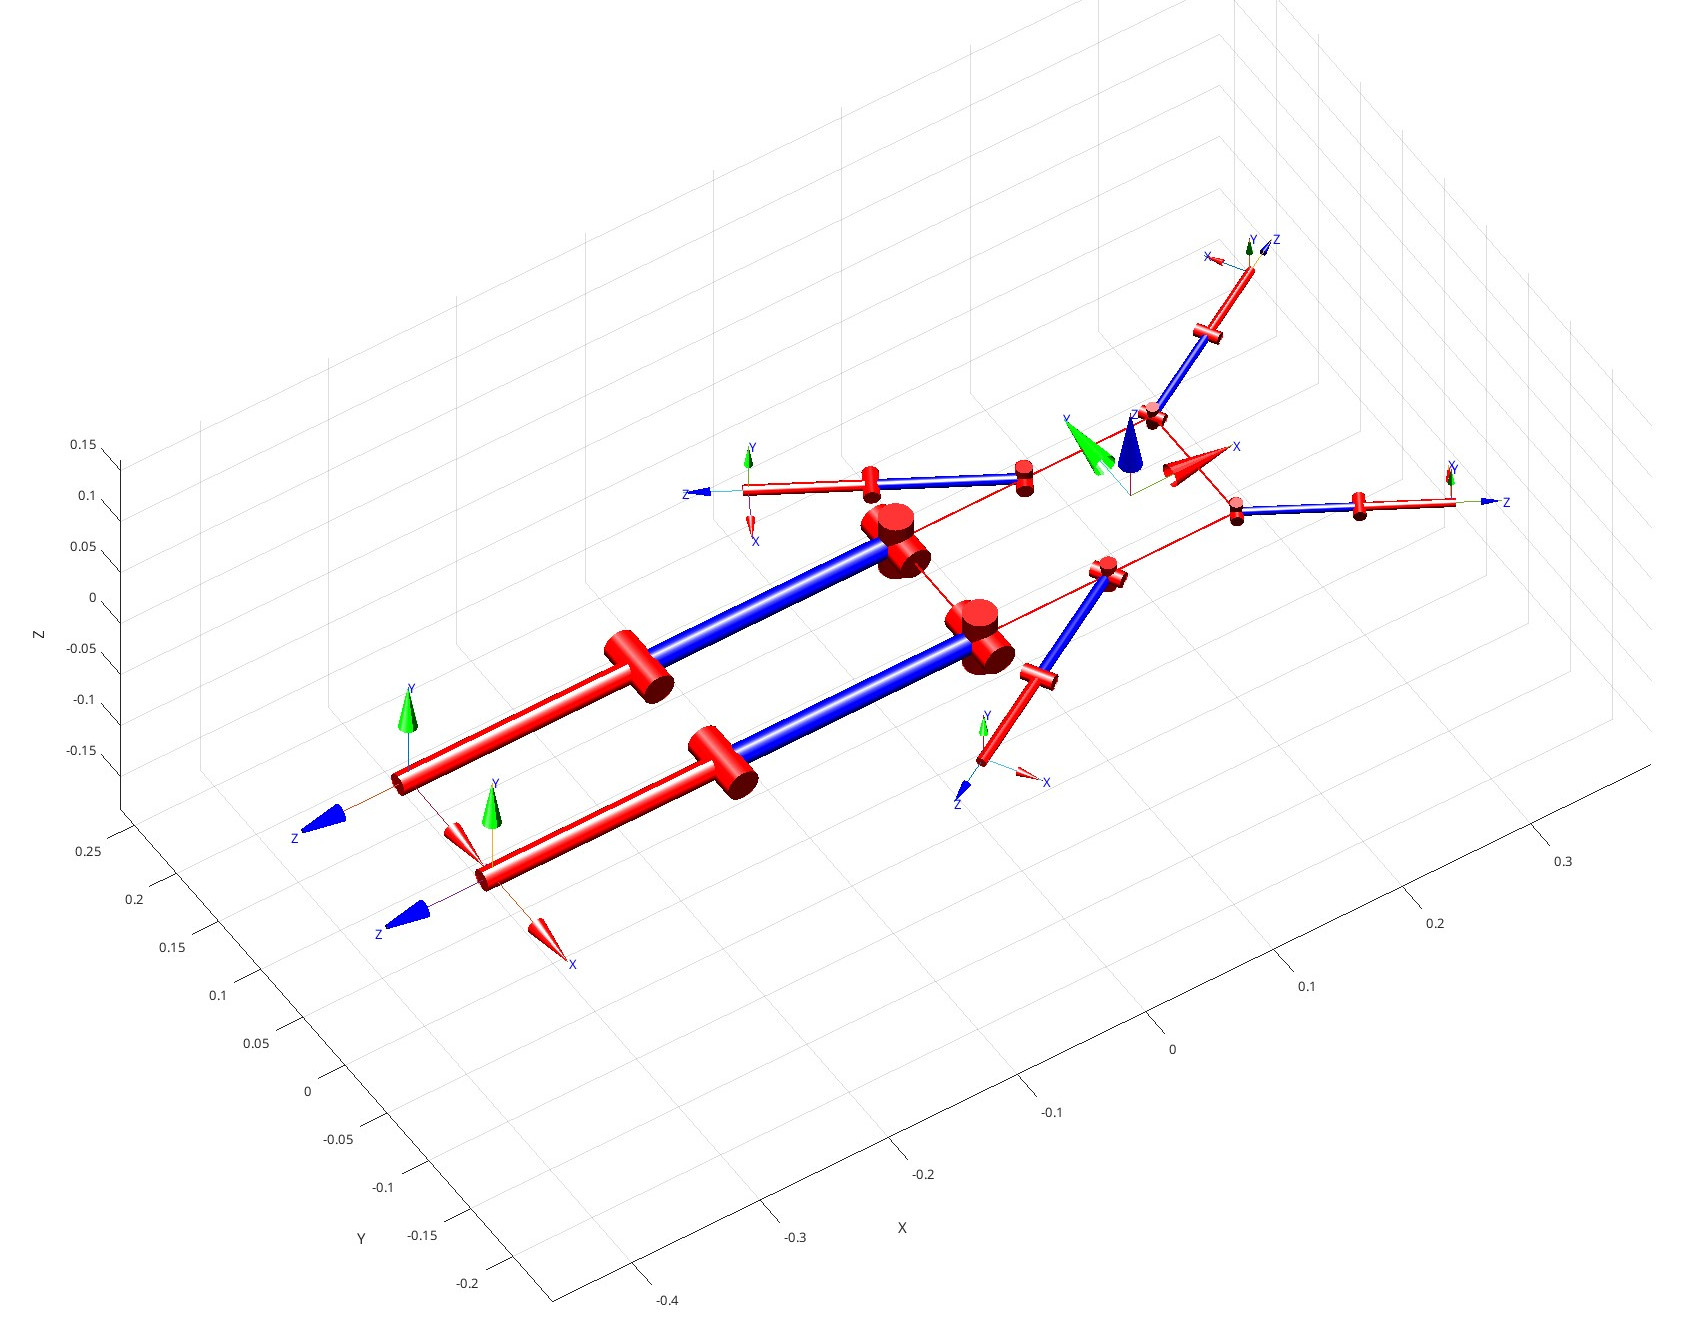
\includegraphics[width=0.7\textwidth]{Images/img_ch3/grasshopper_DH.jpg}
    \caption{Approximated kinematic model of a grasshopper in the zero configuration.}
    \label{fig:grasshopper_model}
\end{figure}

With the model ready to use, the conditions explained before are tested to see if the ATBVME provides meaningful results, in summary the tests are the following: 
\begin{enumerate}
    \setlength\itemsep{-0.7em} 
    \item\label{item:grasshopper_test1}\textbf{Jumping configuration}
    \item\label{item:grasshopper_test2}\textbf{Sensitivity analysis of the jumping configuration}
    \item\label{item:grasshopper_test3}\textbf{One back leg unavailable}
    \item\label{item:grasshopper_test4}\textbf{Both back legs unavailable}
    \item\label{item:grasshopper_test5}\textbf{Sensitivity analysis of CoM position}
\end{enumerate}

To conduct those experiments, first, the different joint velocity limits are considered to use a realistic joint space domain. In particular $\mathbf{Q_{lim}}\in\mathbb{R}^{n\times n}$ is defined \cite{DualArmSpaceManipulabilityEllipsoid}as a diagonal matrix containing the joint limit of all the legs. 
To capture the fact that the front(F) and mid(M) legs are less reactive and used for slow walking, while the back(B) leg's femur-to-tibia joint is the one responsible for the explosive jump (so the fastest one), this aspect is mdeled by defining the limits as:\\
$\mathbf{\dot{q}}_{lim,LF} = \begin{bmatrix}
    0.8 & 0.8 & 0.8
\end{bmatrix}$; 
$\mathbf{\dot{q}}_{lim,LM} = \begin{bmatrix}
    0.8 & 0.8 & 0.8
\end{bmatrix}$; 
$\mathbf{\dot{q}}_{lim,LB} =  \begin{bmatrix}
    1.0 & 1.0 & 4.0
\end{bmatrix}$\\
(with $\mathbf{\dot{q}}_{lim,LF} = \mathbf{\dot{q}}_{lim,RF}$,$\mathbf{\dot{q}}_{lim,LM} = \mathbf{\dot{q}}_{lim,RM}$, $\mathbf{\dot{q}}_{lim,LB} = \mathbf{\dot{q}}_{lim,RB}$)\\

and finally:
$\mathbf{Q}_{lim} = diag(\mathbf{q}_{lim,LF}, \mathbf{q}_{lim,LM}, \mathbf{q}_{lim,LB}, \mathbf{q}_{lim,RF}, \mathbf{q}_{lim,RM}, \mathbf{q}_{lim,RB})$


 because the manipulability theory is relevant to derive the preferred directions rather than the specific numbers\cite{LimitsEllipsoid}, the specific numeric value is not important. Furthermore, this analysis is not rigorous in the exact sizes and dimensions. The important aspect of these boundary values is that the femur-to-tibia joint is the biggest, and the others represent realistic behavior. 

From the definition of $\mathbf{Q}_{lim}$ it is possible to redefine the joint-space sphere behind Yoshikawa's theory in a normalized space $\mathbf{\tilde{\dot{q}}} = \mathbf{Q}^{-1}_{lim}\mathbf{\dot{q}}$, as:
\begin{equation} \mathbf{\tilde{\dot{q}}}^T\mathbf{\tilde{\dot{q}}} = 1
    \label{eq:nornalized_space}
\end{equation}

Then it is simple to rewrite all in the joint space and obtain a new quadratic form for the manipulability ellipsoid, including different symmetric joint limits. In this way, it is possible to give more importance to some of the joints rather than others, solving a limitation of the manipulability theory.  

\textbf{1) Jumping Configuration}\\
In this configuration\cite{Grasshopper3}, the legs are considered with the following joint values, as reported in figure \ref{fig:jumping_config} : 

\begin{equation}
    \label{eq:jumping_config}
    \left\{
    \begin{aligned}
           \mathbf{q}_{LF} = \mathbf{q}_{RF}  = \begin{bmatrix}
               0 &-\frac{\pi}{6} & \frac{2}{3}\pi 
           \end{bmatrix}^T = \begin{bmatrix}
               0 &-30^\circ & 120^\circ 
           \end{bmatrix}^T 
           \\
           \mathbf{q}_{LM} = \mathbf{q}_{RM}  = \begin{bmatrix}
               0 &-\frac{\pi}{6} & \frac{2}{3}\pi 
           \end{bmatrix}^T = \begin{bmatrix}
                0 &-30^\circ & 120^\circ
           \end{bmatrix}^T 
            \\
            \mathbf{q}_{LB} = \mathbf{q}_{RB}  = \begin{bmatrix}
               -\frac{\pi}{12} &-\frac{7}{36}\pi & \frac{8}{9}\pi 
           \end{bmatrix}^T = \begin{bmatrix}
               -15^\circ &-35^\circ & 160^\circ
           \end{bmatrix}^T 
    \end{aligned}
    \right.
\end{equation}

It is evident from the shape of the ATBVME reported in Fig.\ref{fig:jumping_ME_ortho} and \ref{fig:jumping_ME_xz} that a clear jumping direction is indicated by the bigger axis of the ellipsoid, where higher base velocity is achievable. 

\begin{figure}[H]
    \centering
    \subfloat[Jumping configuration\label{fig:jumping_config}]{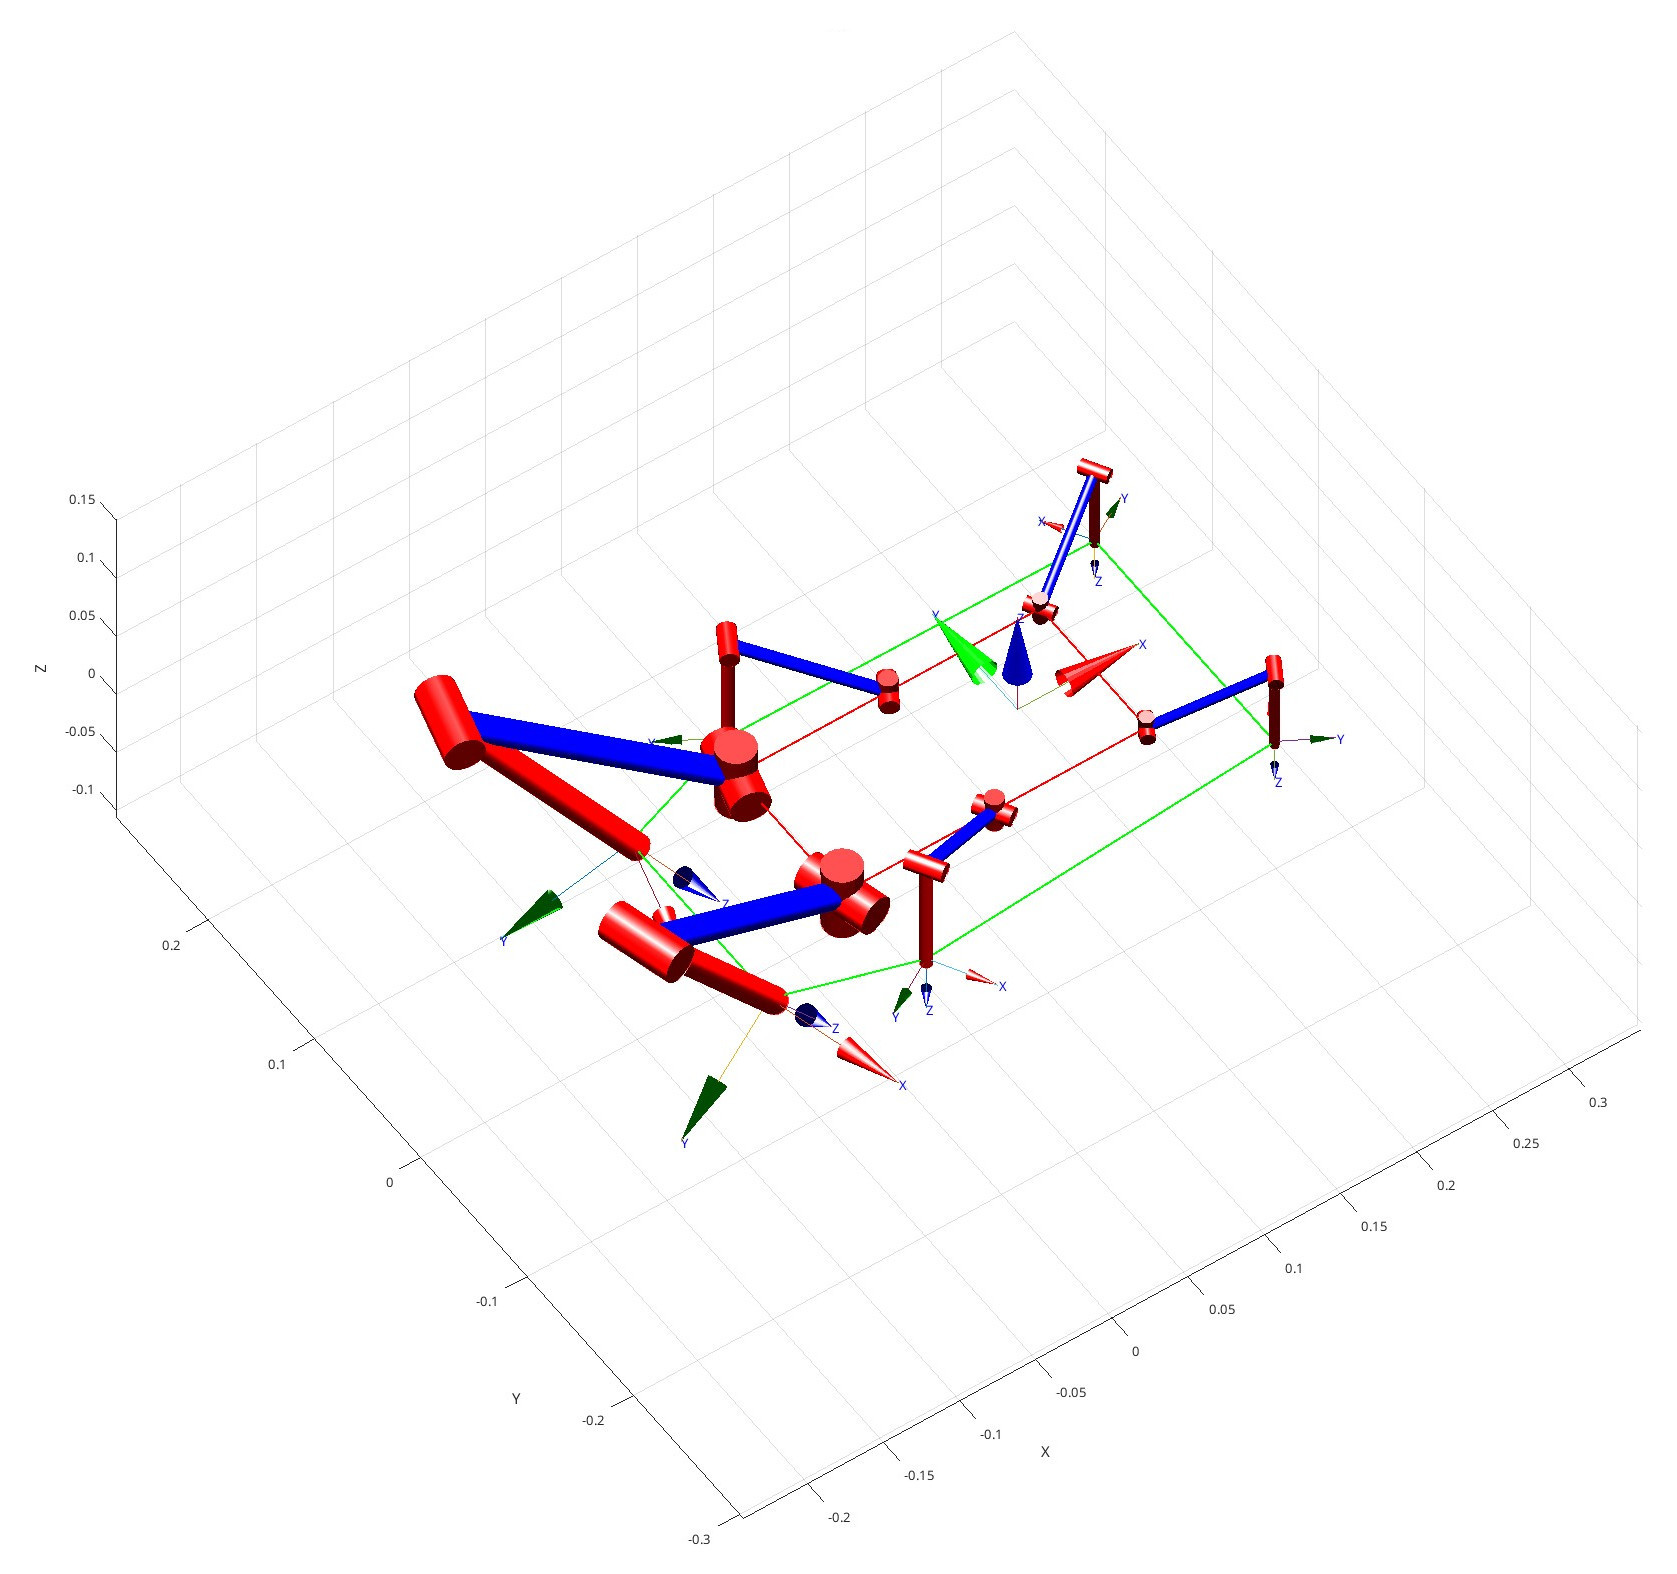
\includegraphics[width=0.5\textwidth]{Images/img_ch3/jumping_config.jpg}}
    \subfloat[ATBVME and legs BVME, orthographic view\label{fig:jumping_ME_ortho}]
    {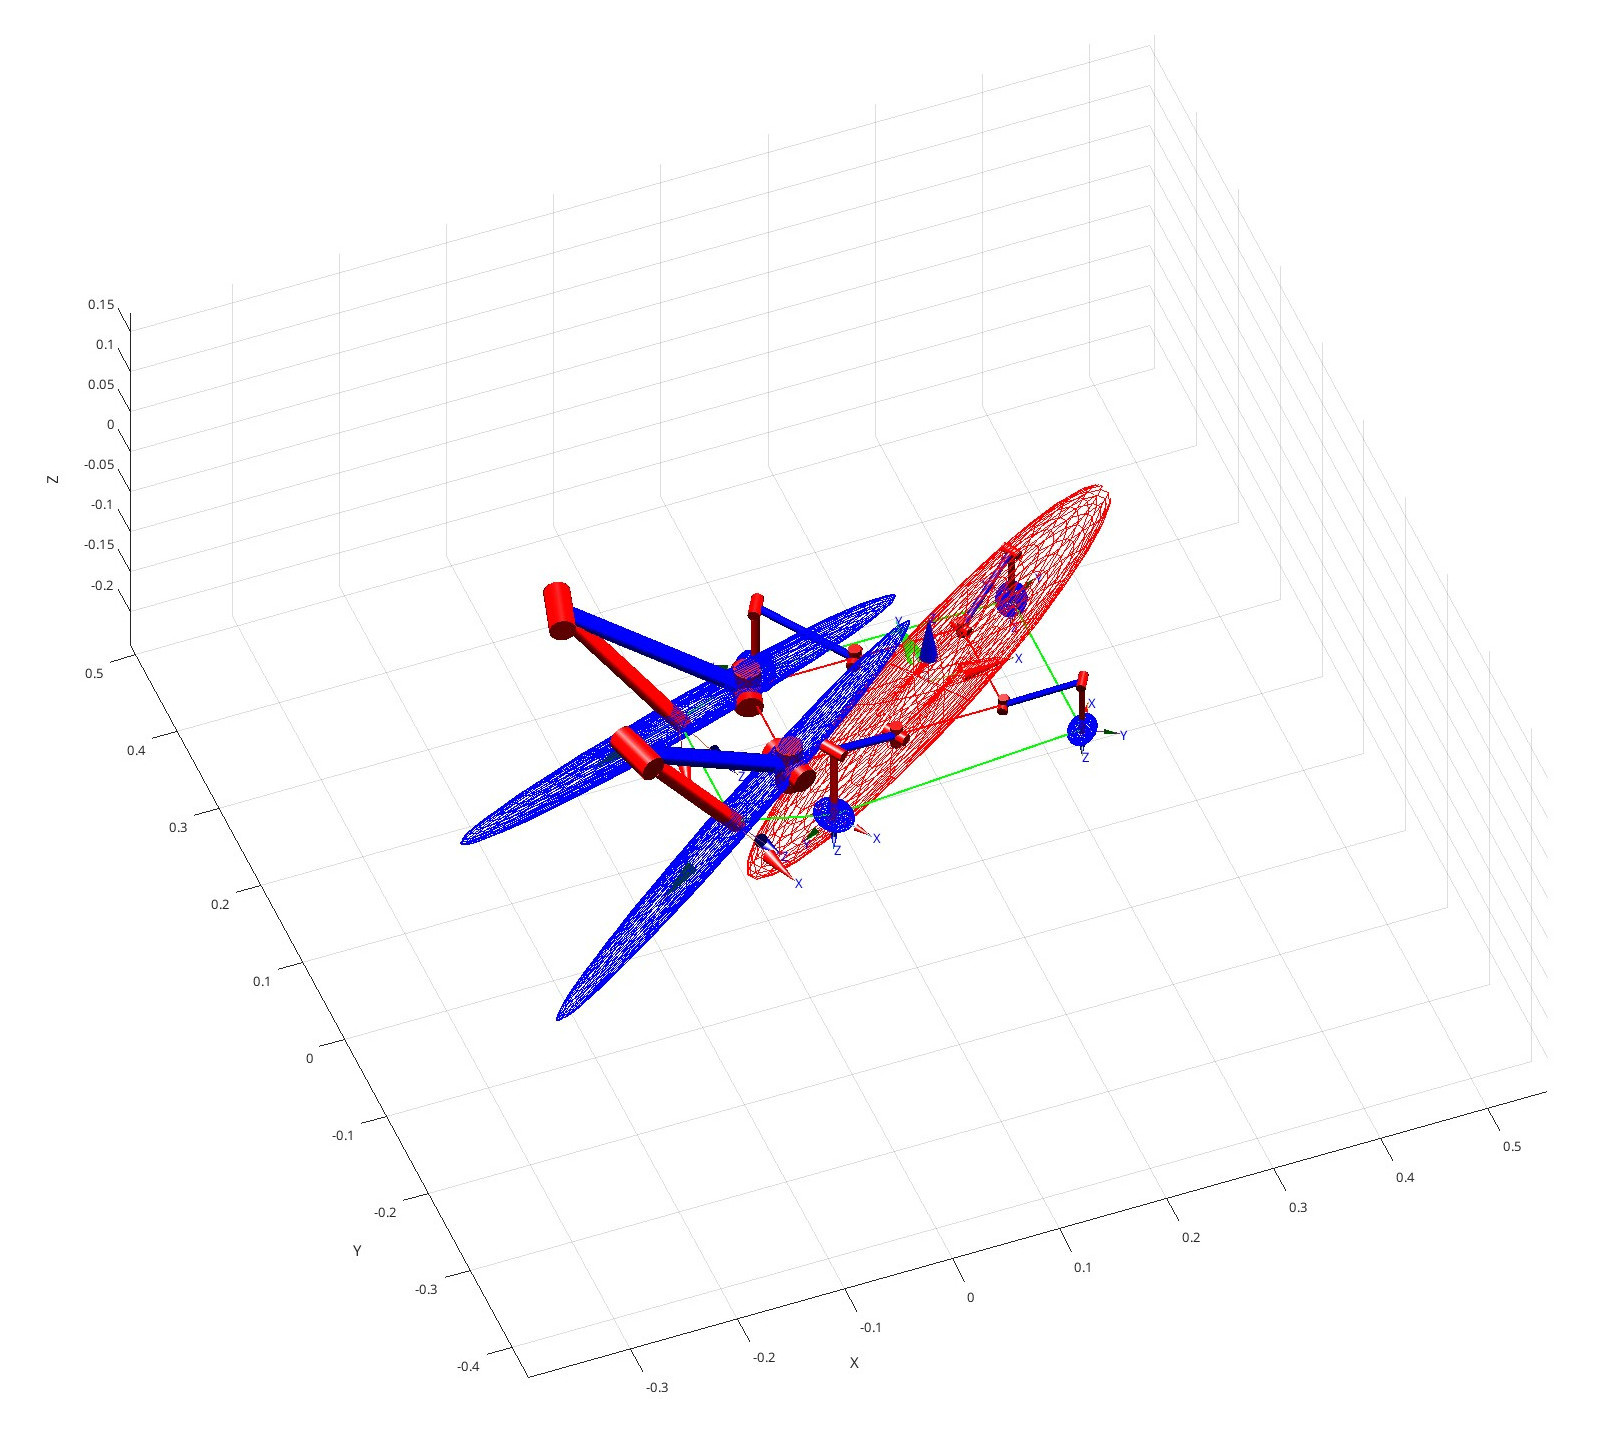
\includegraphics[width=0.5\textwidth]{Images/img_ch3/jumping_ME_ortho.jpg}}\\
    \subfloat[ATBVME and legs BVME, xz view\label{fig:jumping_ME_xz}]
    {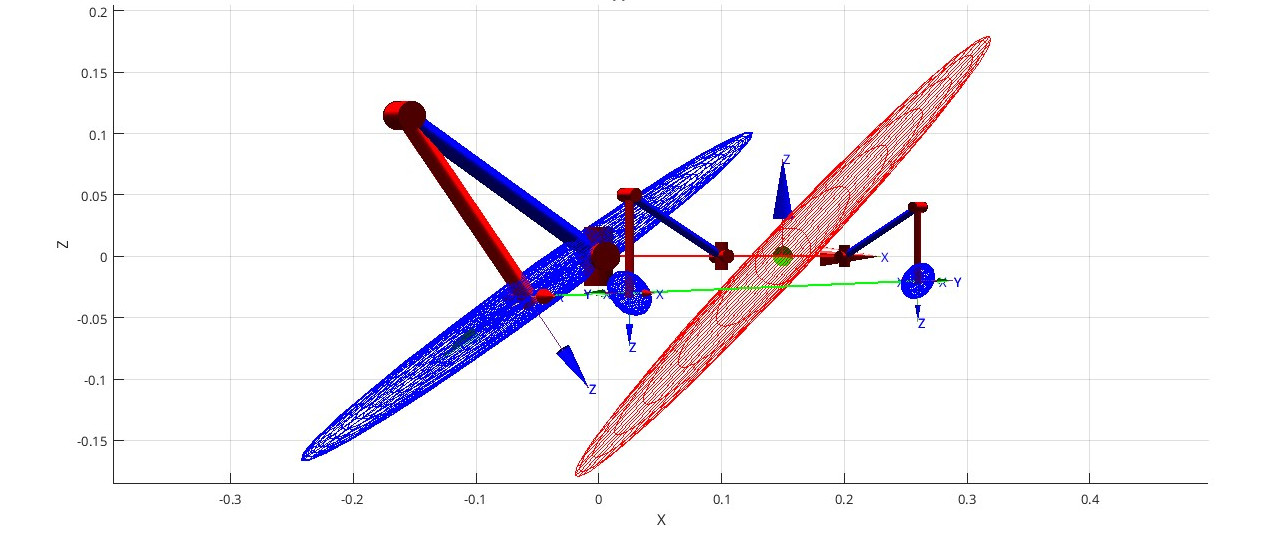
\includegraphics[width=0.6\textwidth]{Images/img_ch3/jumping_ME_xz.jpg}}
    \caption[Manipulability analysis in the jumping configuration]{Manipulability analysis in the jumping configuration}
    \label{fig:grasshopper_model}
\end{figure}


\textbf{2) Jumping Configuration, Sensitivity Analysis}\\
The changes in the ATBVME, when different back leg configurations are considered, are interesting to analyze if the results are consistent with the real biomechanics. 

The jumping configuration of the grasshopper is not only the one in (\ref{eq:jumping_config}), but a set of configurations around the one previously defined, according to the desired jump direction. Releasing the femur-to-tibia (F2T) joint should change the "explosive motion direction". As a limitation of a pure kinematic model, here the spring-like behavior of the extensor muscle is not modeled as a reaction to contraction release, but with the higher speed limit of the F2T joint. For this reason, even when not contracted, back legs give a high-velocity manipulability effect, but configurations far from the jumping one are expected to be disadvantages for this task. 

The results in changing the coxa-to-femur (C2F) and femur-to-tibia (F2T) are reported in Fig.\ref{fig:jumping_changes} in configurations where the back legs touches the ground. Finally, uncommon configurations with wider back legs (B2C angles sensitivity) are reported in Fig.\ref{fig:b2c_changes}, highlighting why these are not common configurations. 


\begin{figure}[H]
    \centering
    \subfloat[$C2F=-30^\circ$, $C2F=160^\circ$, xy view\label{fig:jumping_neg30_160_xy}]{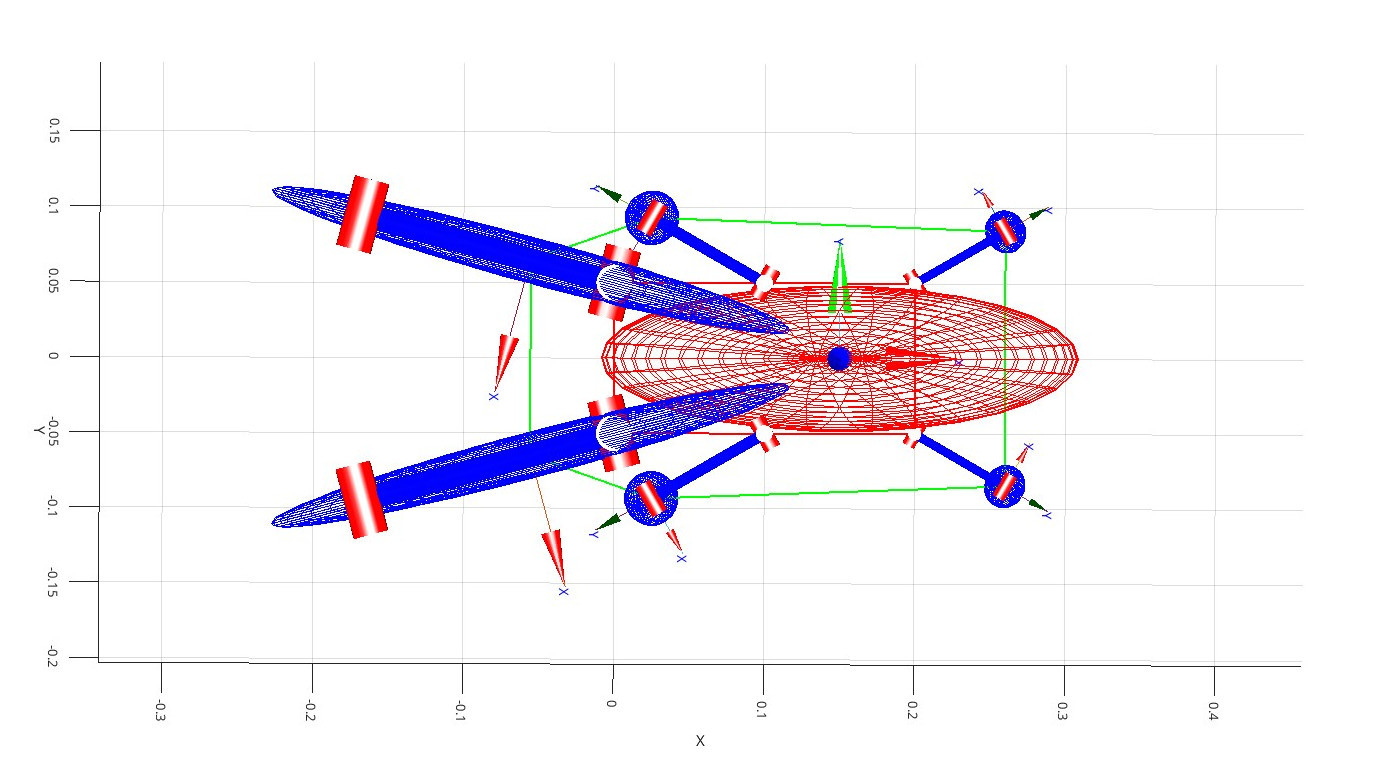
\includegraphics[width=0.50\textwidth]{Images/img_ch3/jumping_neg30_160_xy.jpg}}
    \subfloat[$C2F=-30^\circ$, $C2F=160^\circ$, xz view\label{fig:jumping_neg30_160}]{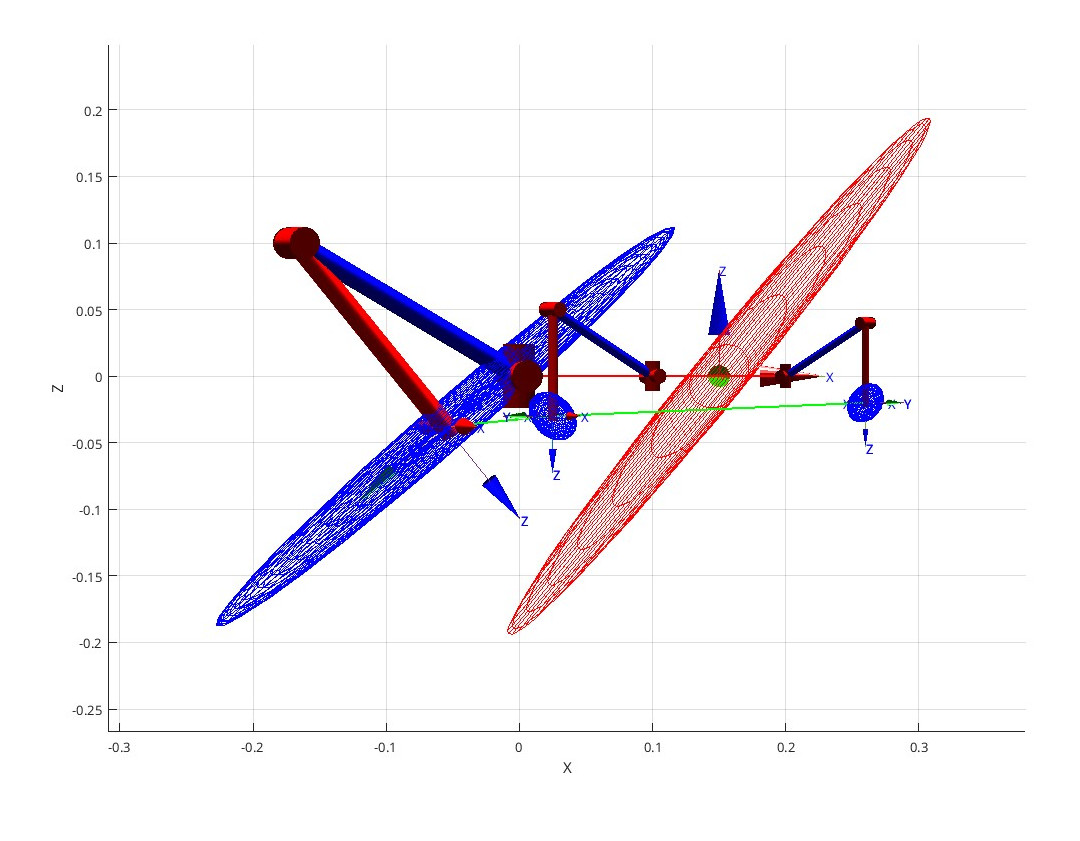
\includegraphics[width=0.45\textwidth]{Images/img_ch3/jumping_neg30_160.jpg}}\\
    \subfloat[$C2F=-20^\circ$, $C2F=170^\circ$, xz view\label{fig:jumping_neg20_170}]
    {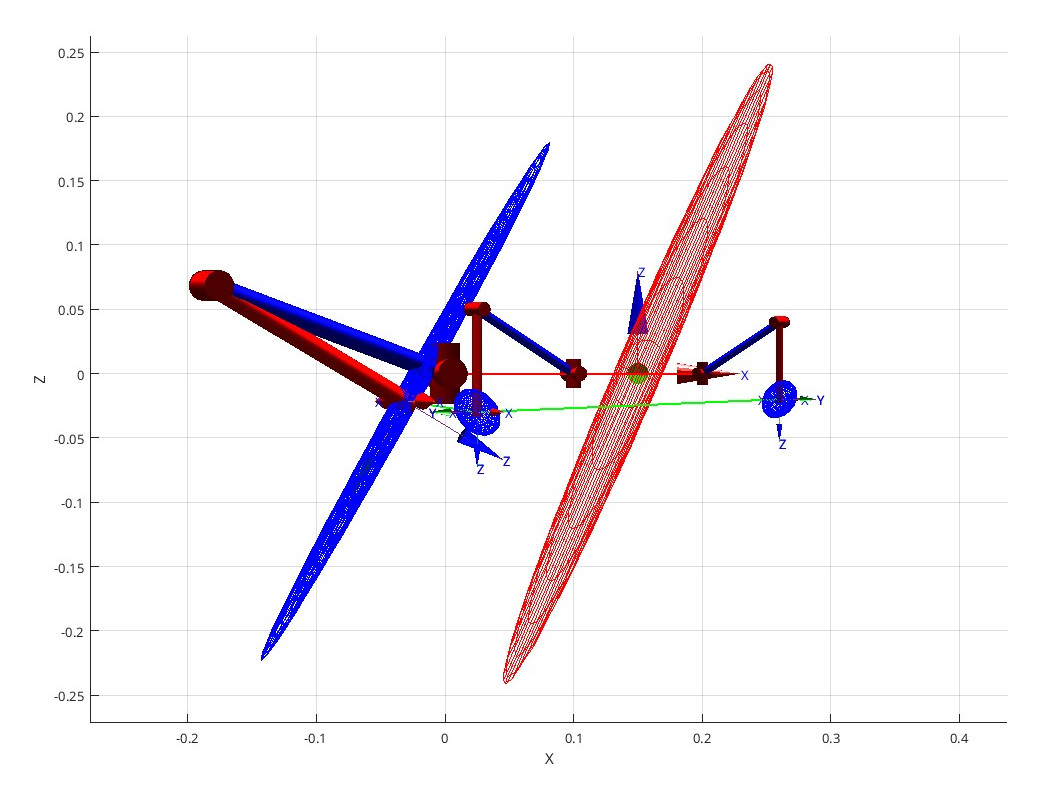
\includegraphics[width=0.45\textwidth]{Images/img_ch3/jumping_neg20_170.jpg}}
    \subfloat[$C2F=-20^\circ$, $C2F=50^\circ$, xz view\label{fig:jumping_neg20_50}]
    {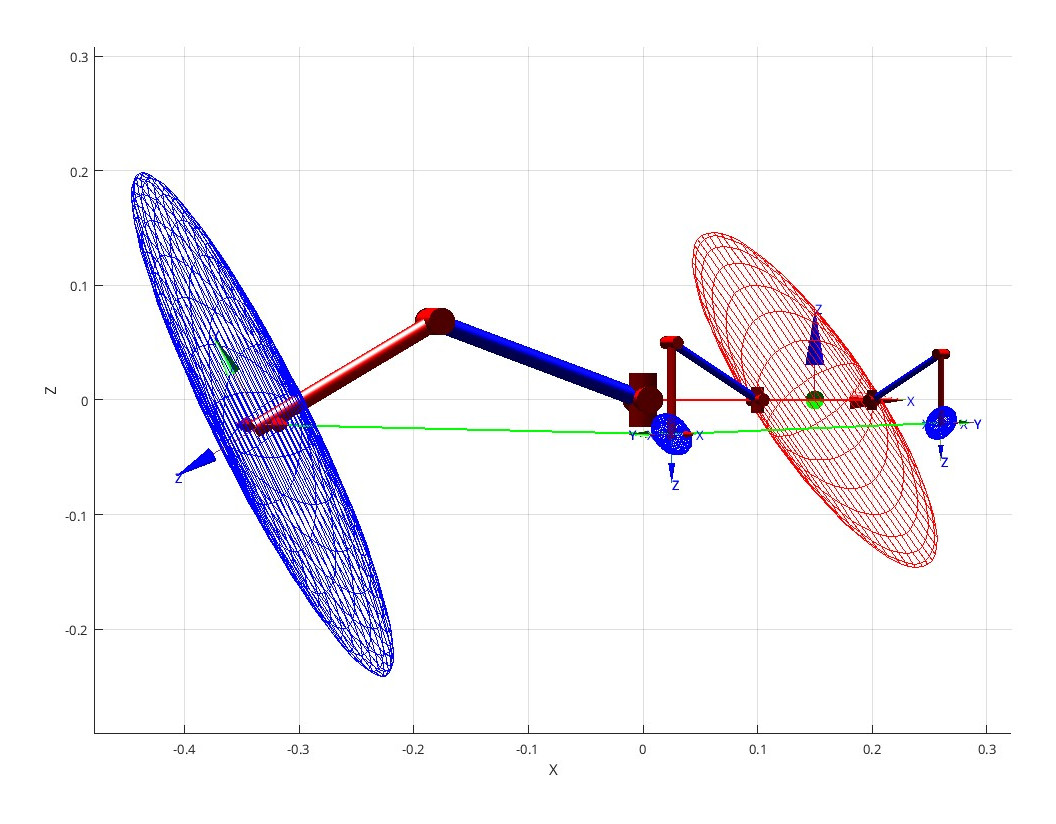
\includegraphics[width=0.45\textwidth]{Images/img_ch3/jumping_neg20_50.jpg}}
    \caption[C2F and F2T jumping sensitivity]{C2F and F2T jumping sensitivity, maintaining $B2C=-15^\circ$.}
    \label{fig:jumping_changes}
\end{figure}

In all the configurations tested and reported above in Fig.\ref{fig:jumping_changes}, the ellipsoid is oriented in the x-axis direction, but the major axis highly depends on the back legs configuration. 
Different legs' interactions with the ground (here modeled just kinematically by the configurations) affect the jump performances and the direction. 

Intuitively, if the back legs are wider, jumping capability gets distributed in a wider range of directions, using efficiency, and the BME is coherent with this, as reported in Fig.\ref{fig:b2c_changes}.

In conclusion, an asymmetric configuration of the back legs is reported in Fig.\ref{fig:asymmetry}, resulting in consistent ellipsoids with the expected unnatural jumping capability.

\begin{figure}[H]
    \centering
    \subfloat[$|B2C|=15^\circ$\label{fig:jumping_b2c_neg15}]{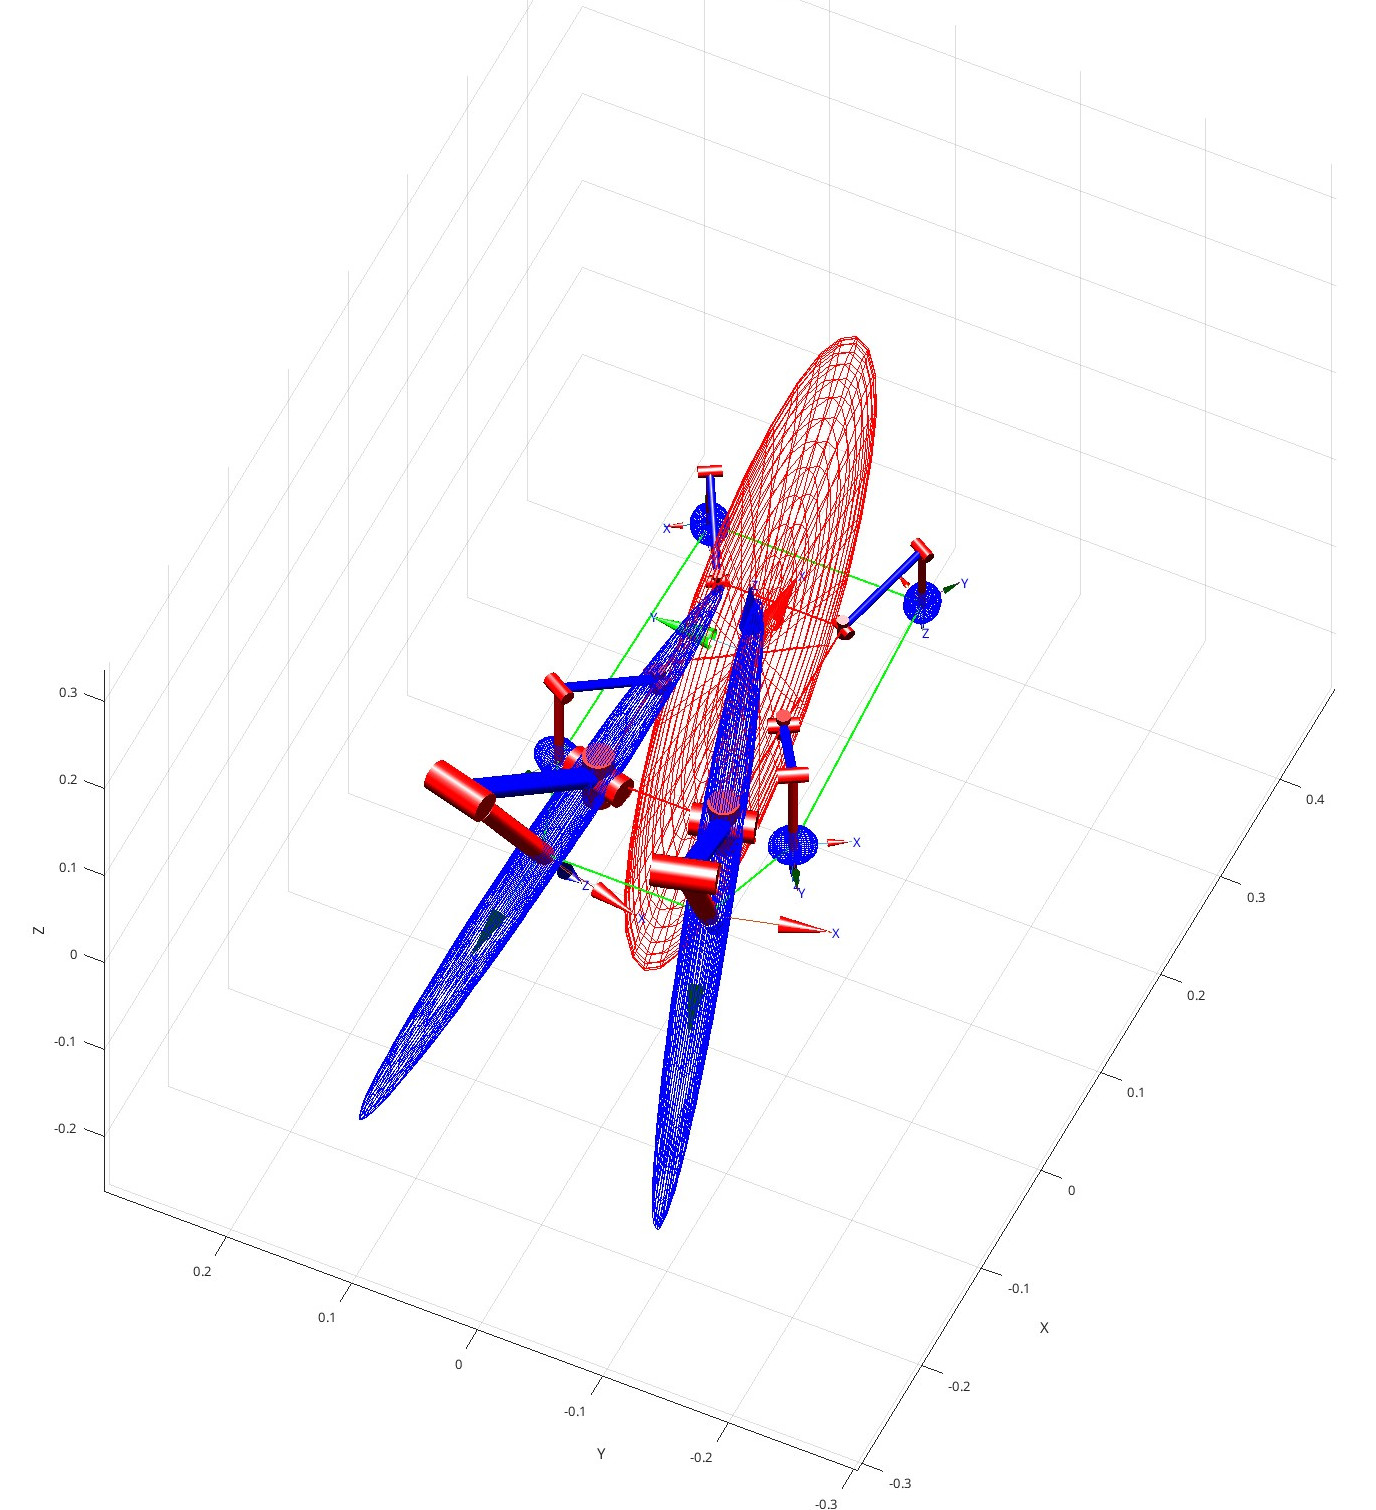
\includegraphics[width=0.4\textwidth]{Images/img_ch3/jumping_b2c_neg15.jpg}}
    \subfloat[$|B2C|=25^\circ$\label{fig:jumping_b2c_neg25}]
    {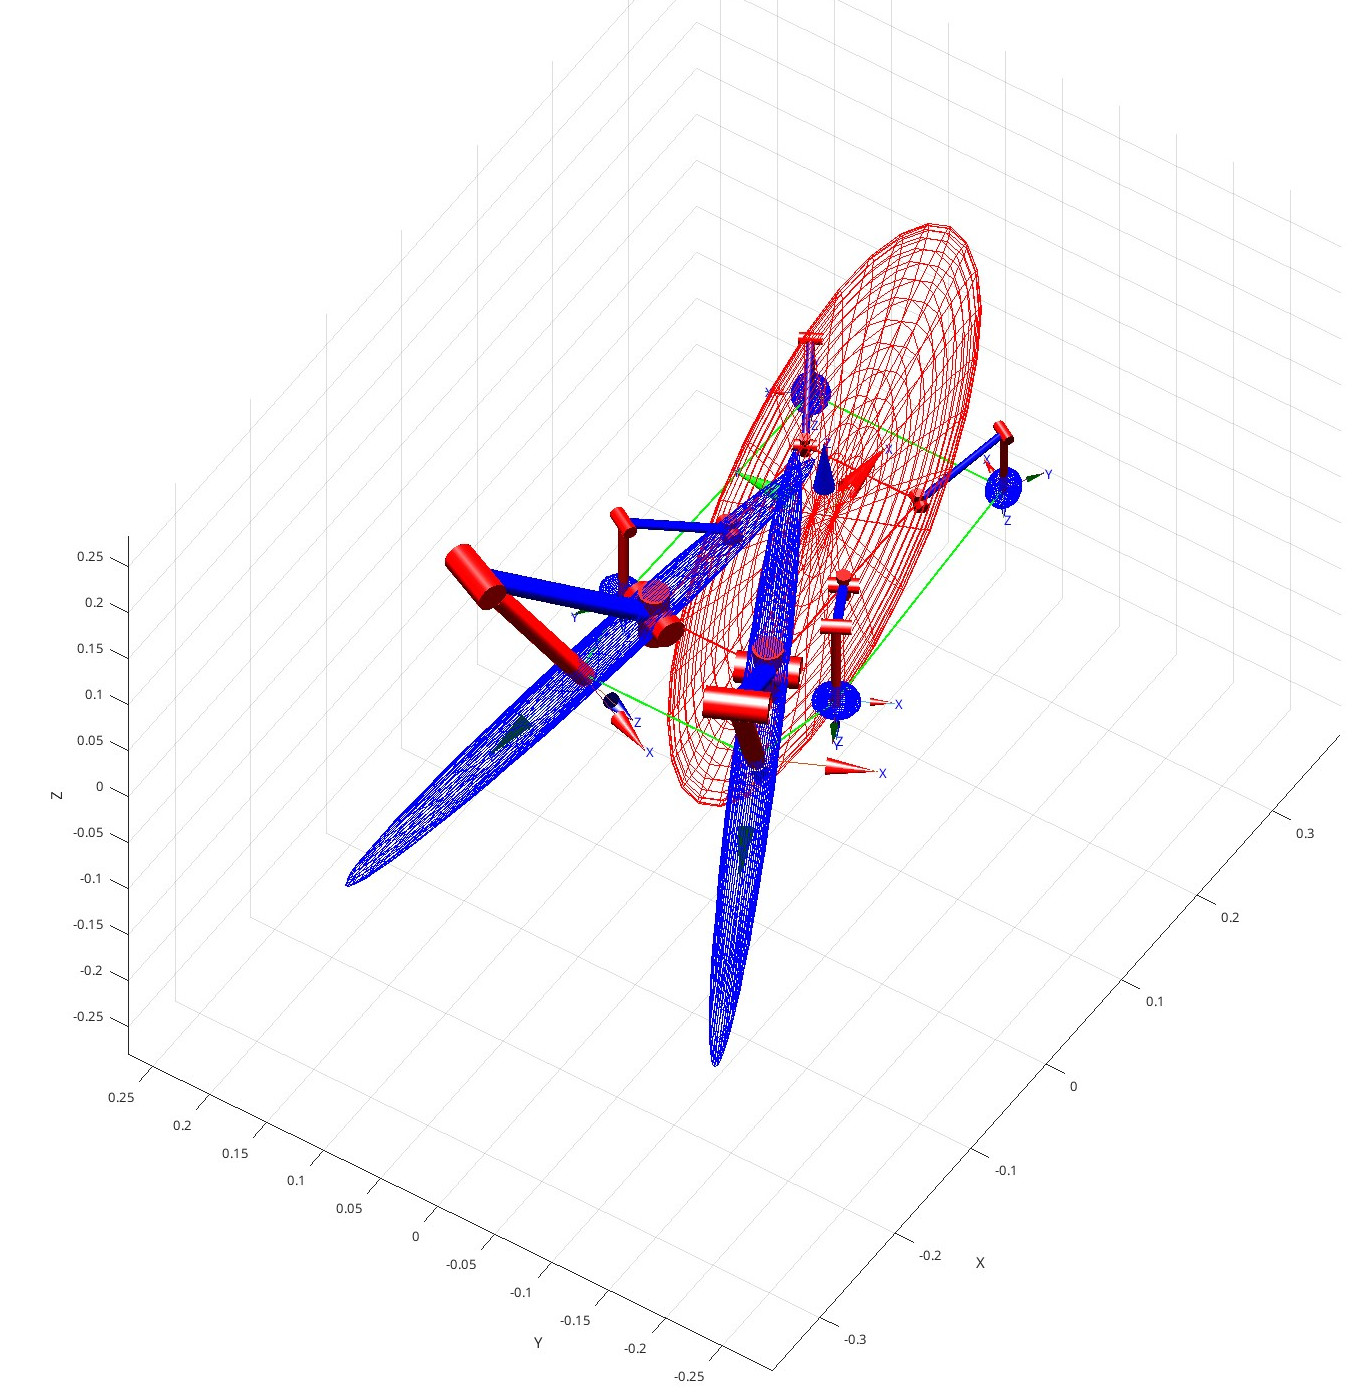
\includegraphics[width=0.4\textwidth]{Images/img_ch3/jumping_b2c_neg25.jpg}}\\
    \subfloat[$|B2C|=45^\circ$\label{fig:jumping_b2c_neg45}]
    {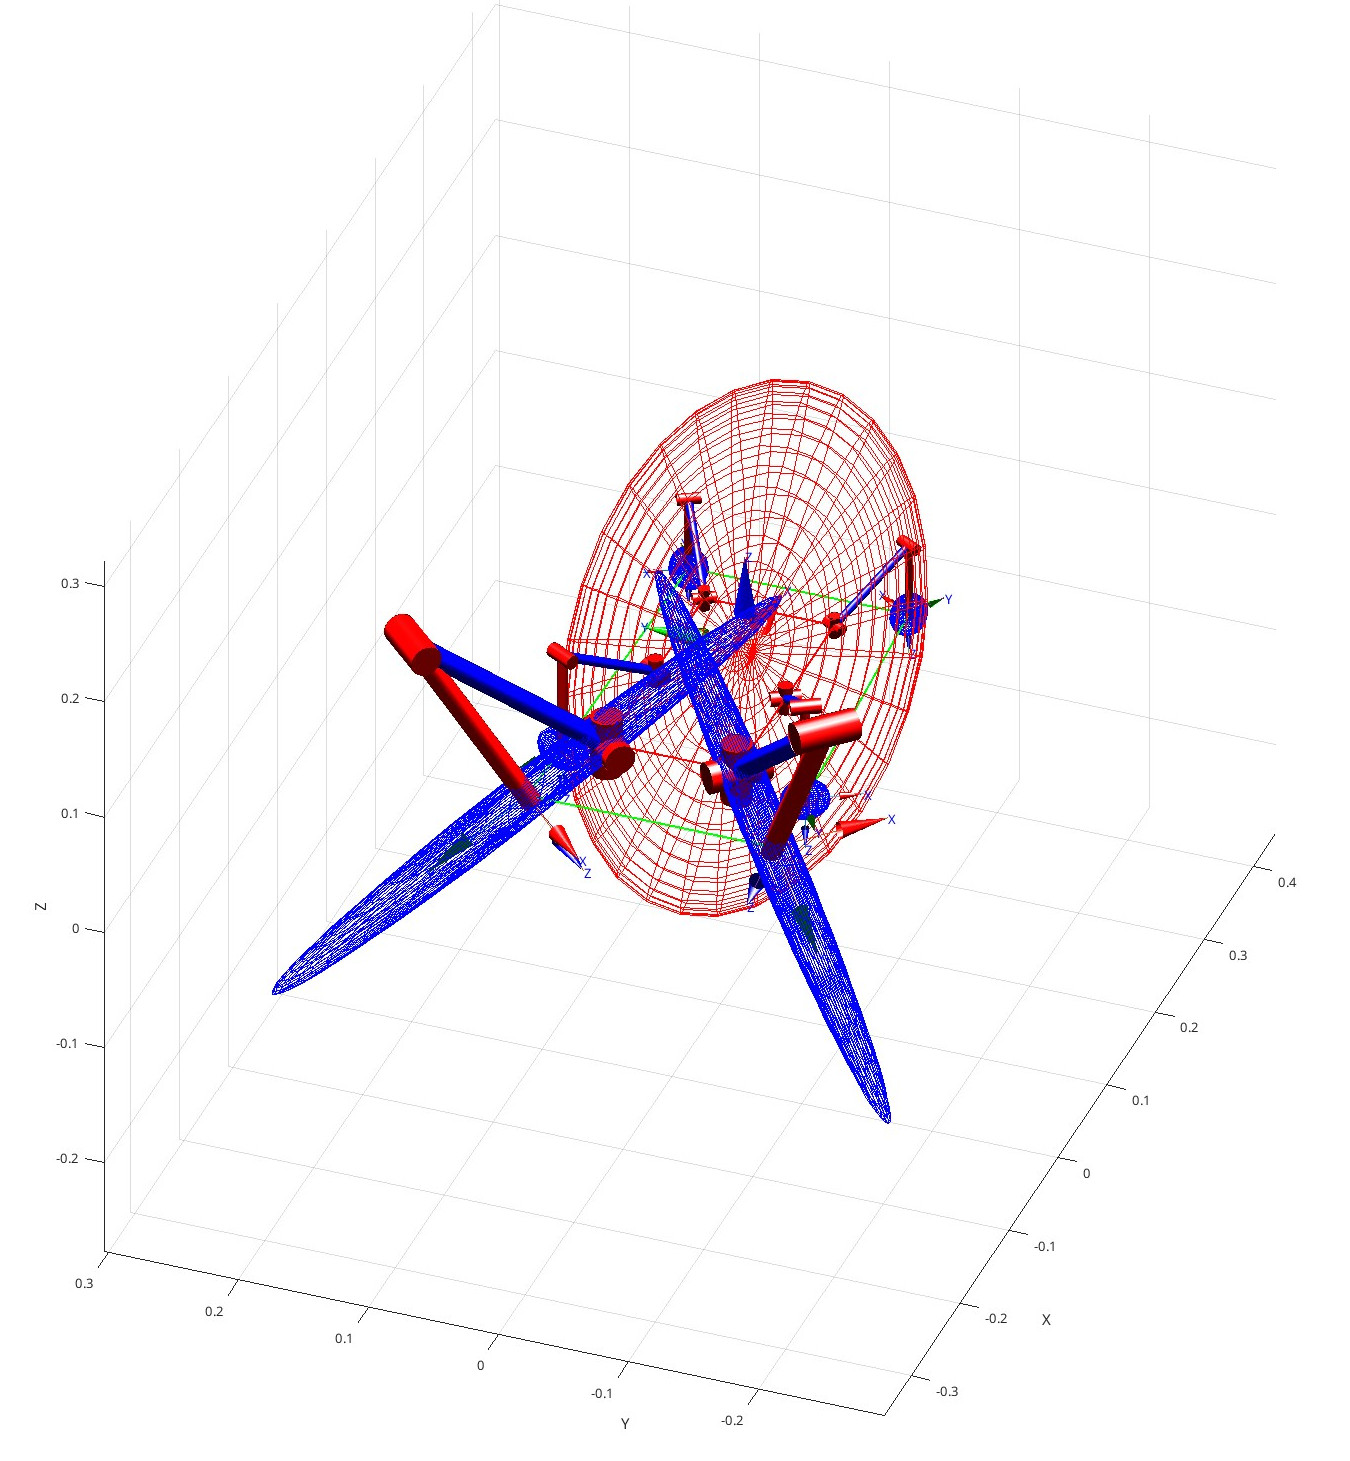
\includegraphics[width=0.4\textwidth]{Images/img_ch3/jumping_b2c_neg45.jpg}}
    \subfloat[$|B2C|=70^\circ$\label{fig:jumping_b2c_neg70}]
    {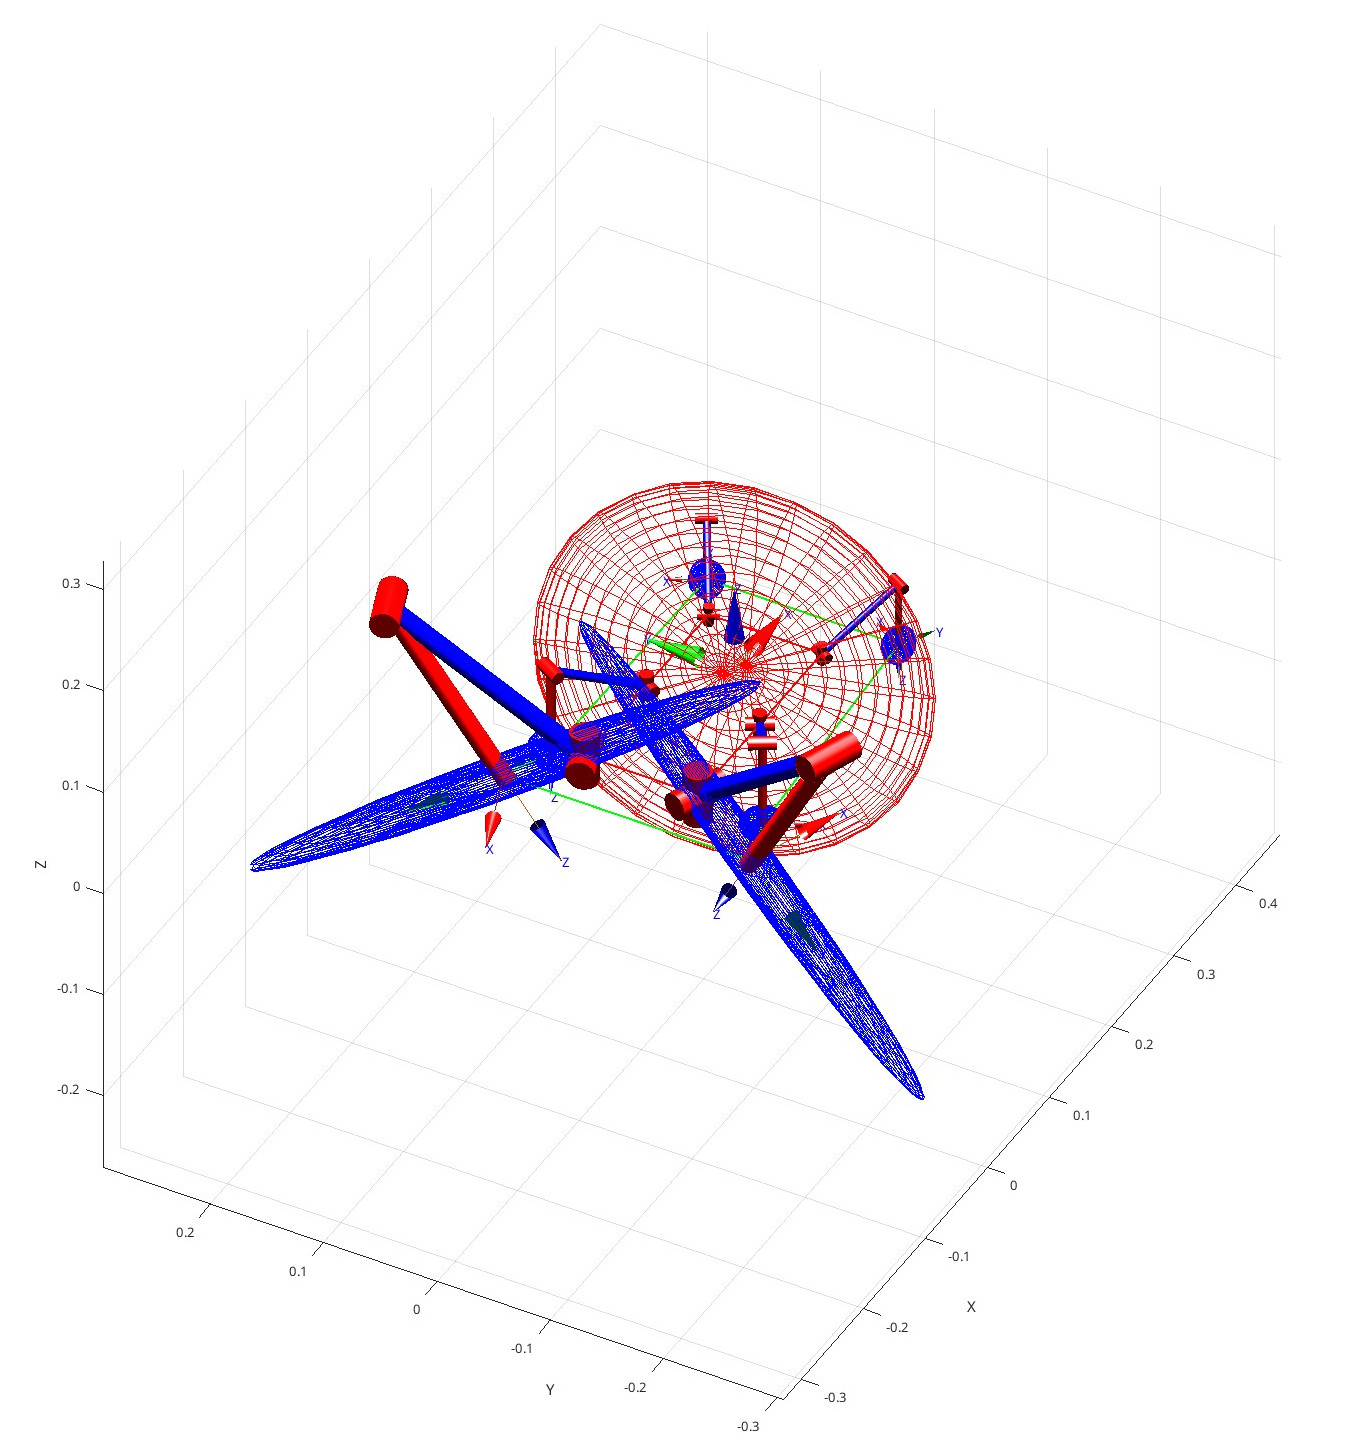
\includegraphics[width=0.4\textwidth]{Images/img_ch3/jumping_b2c_neg70.jpg}}\\
    \subfloat[$|B2C|=15^\circ$, yz view\label{fig:jumping_b2c_neg15_yz}]
    {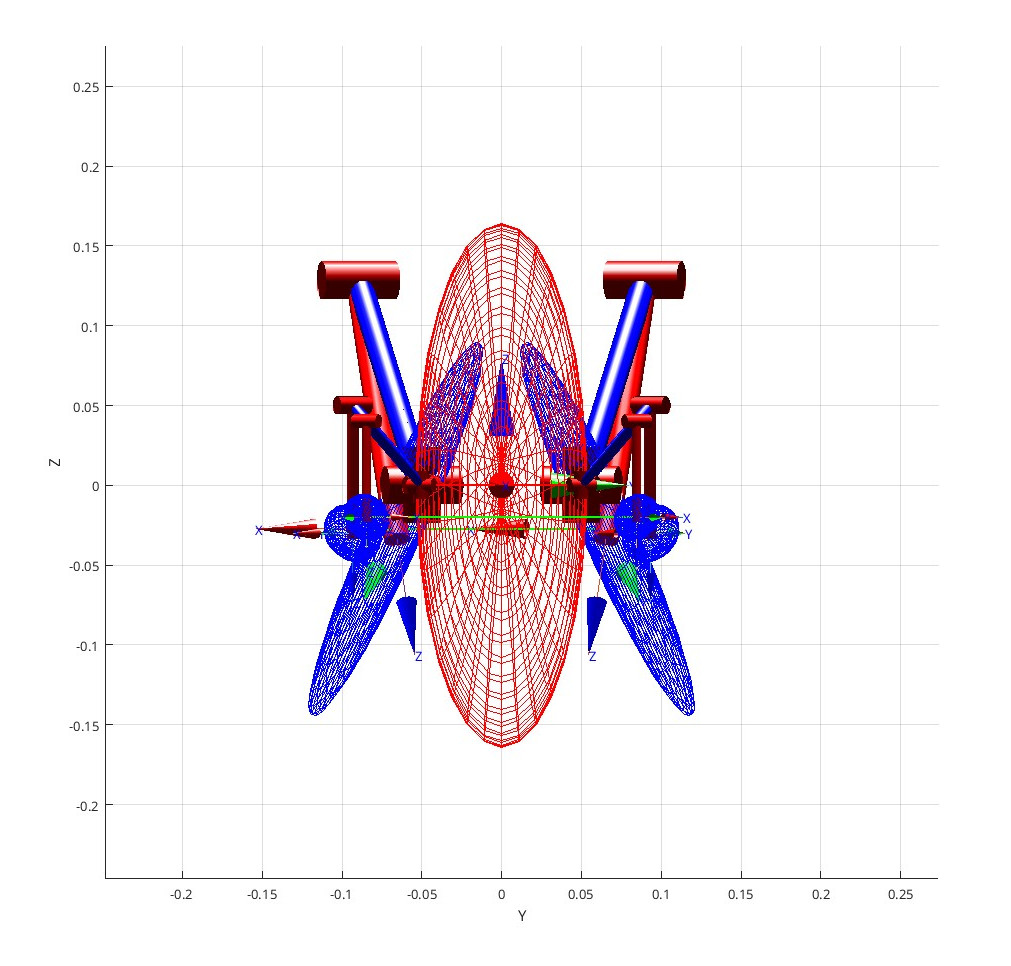
\includegraphics[width=0.4\textwidth]{Images/img_ch3/jumping_b2c_neg15_yz.jpg}}
    \subfloat[$|B2C|=70^\circ$, yz view\label{fig:jumping_b2c_neg70_yz}]
    {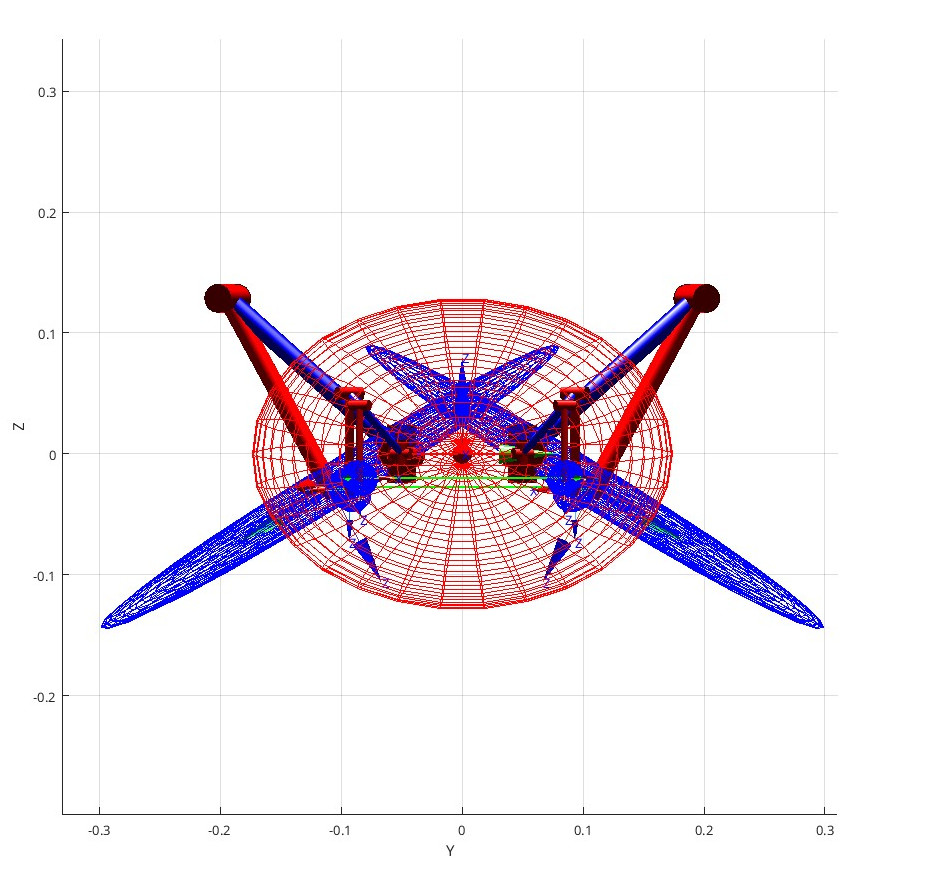
\includegraphics[width=0.4\textwidth]{Images/img_ch3/jumping_b2c_neg70_yz.jpg}}
    \caption[B2C jumping sensitivity]{B2C jumping sensitivity, maintaining $C2F=-40^\circ$ and $F2T=160^\circ$}
    \label{fig:b2c_changes}
\end{figure}

\begin{figure}[H]
    \centering
    \subfloat[$L_{F2T}=120^\circ$ $R_{F2T}=160^\circ$\label{fig:jumping_Lf2t_120_Rf2t_160}]{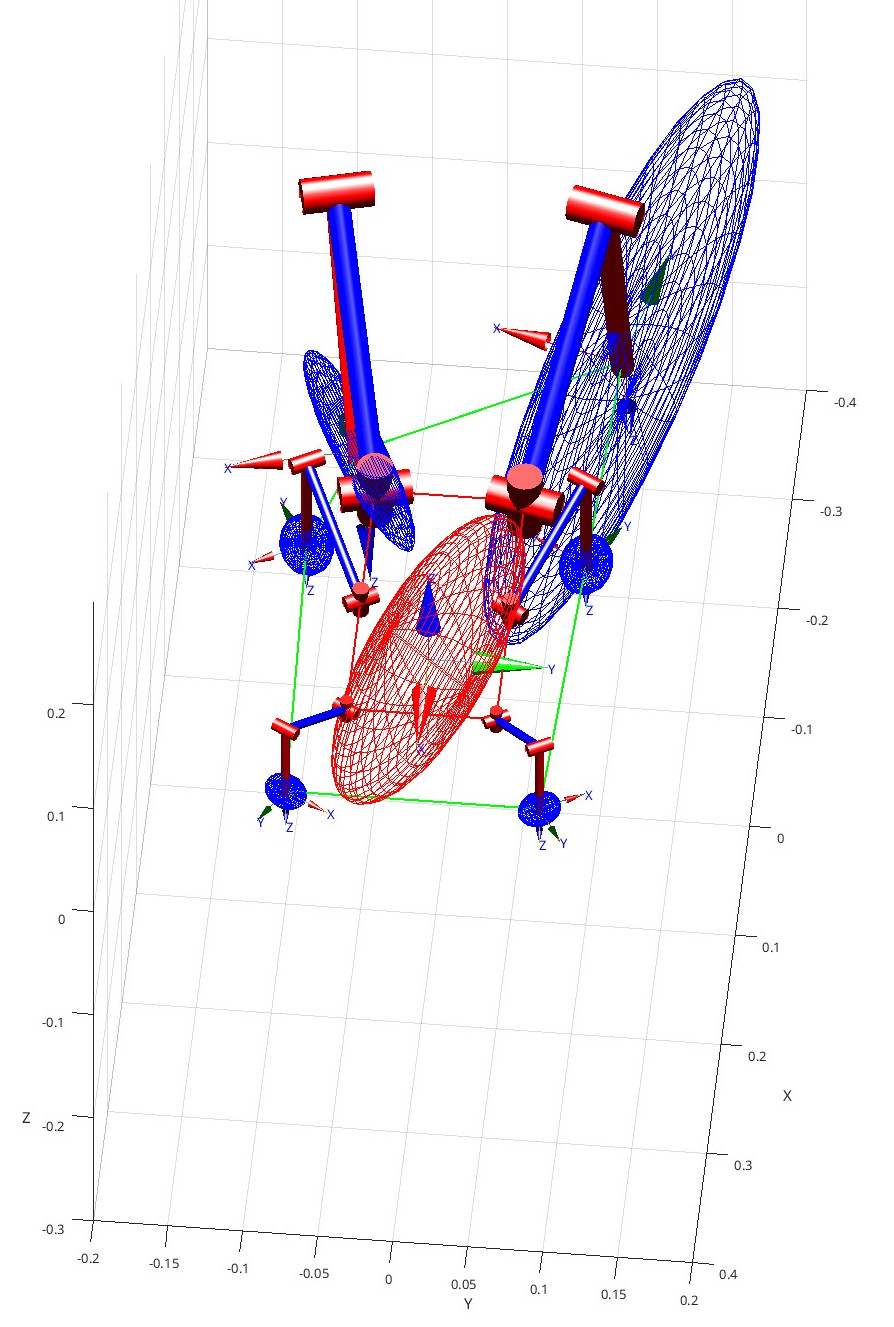
\includegraphics[width=0.35\textwidth]{Images/img_ch3/jumping_Lf2t_120_Rf2t_160.jpg}}
    \subfloat[$L_{F2T}=120^\circ$ $R_{F2T}=160^\circ$, yz view\label{fig:jumping_Lf2t_120_Rf2t_160_yz}]
    {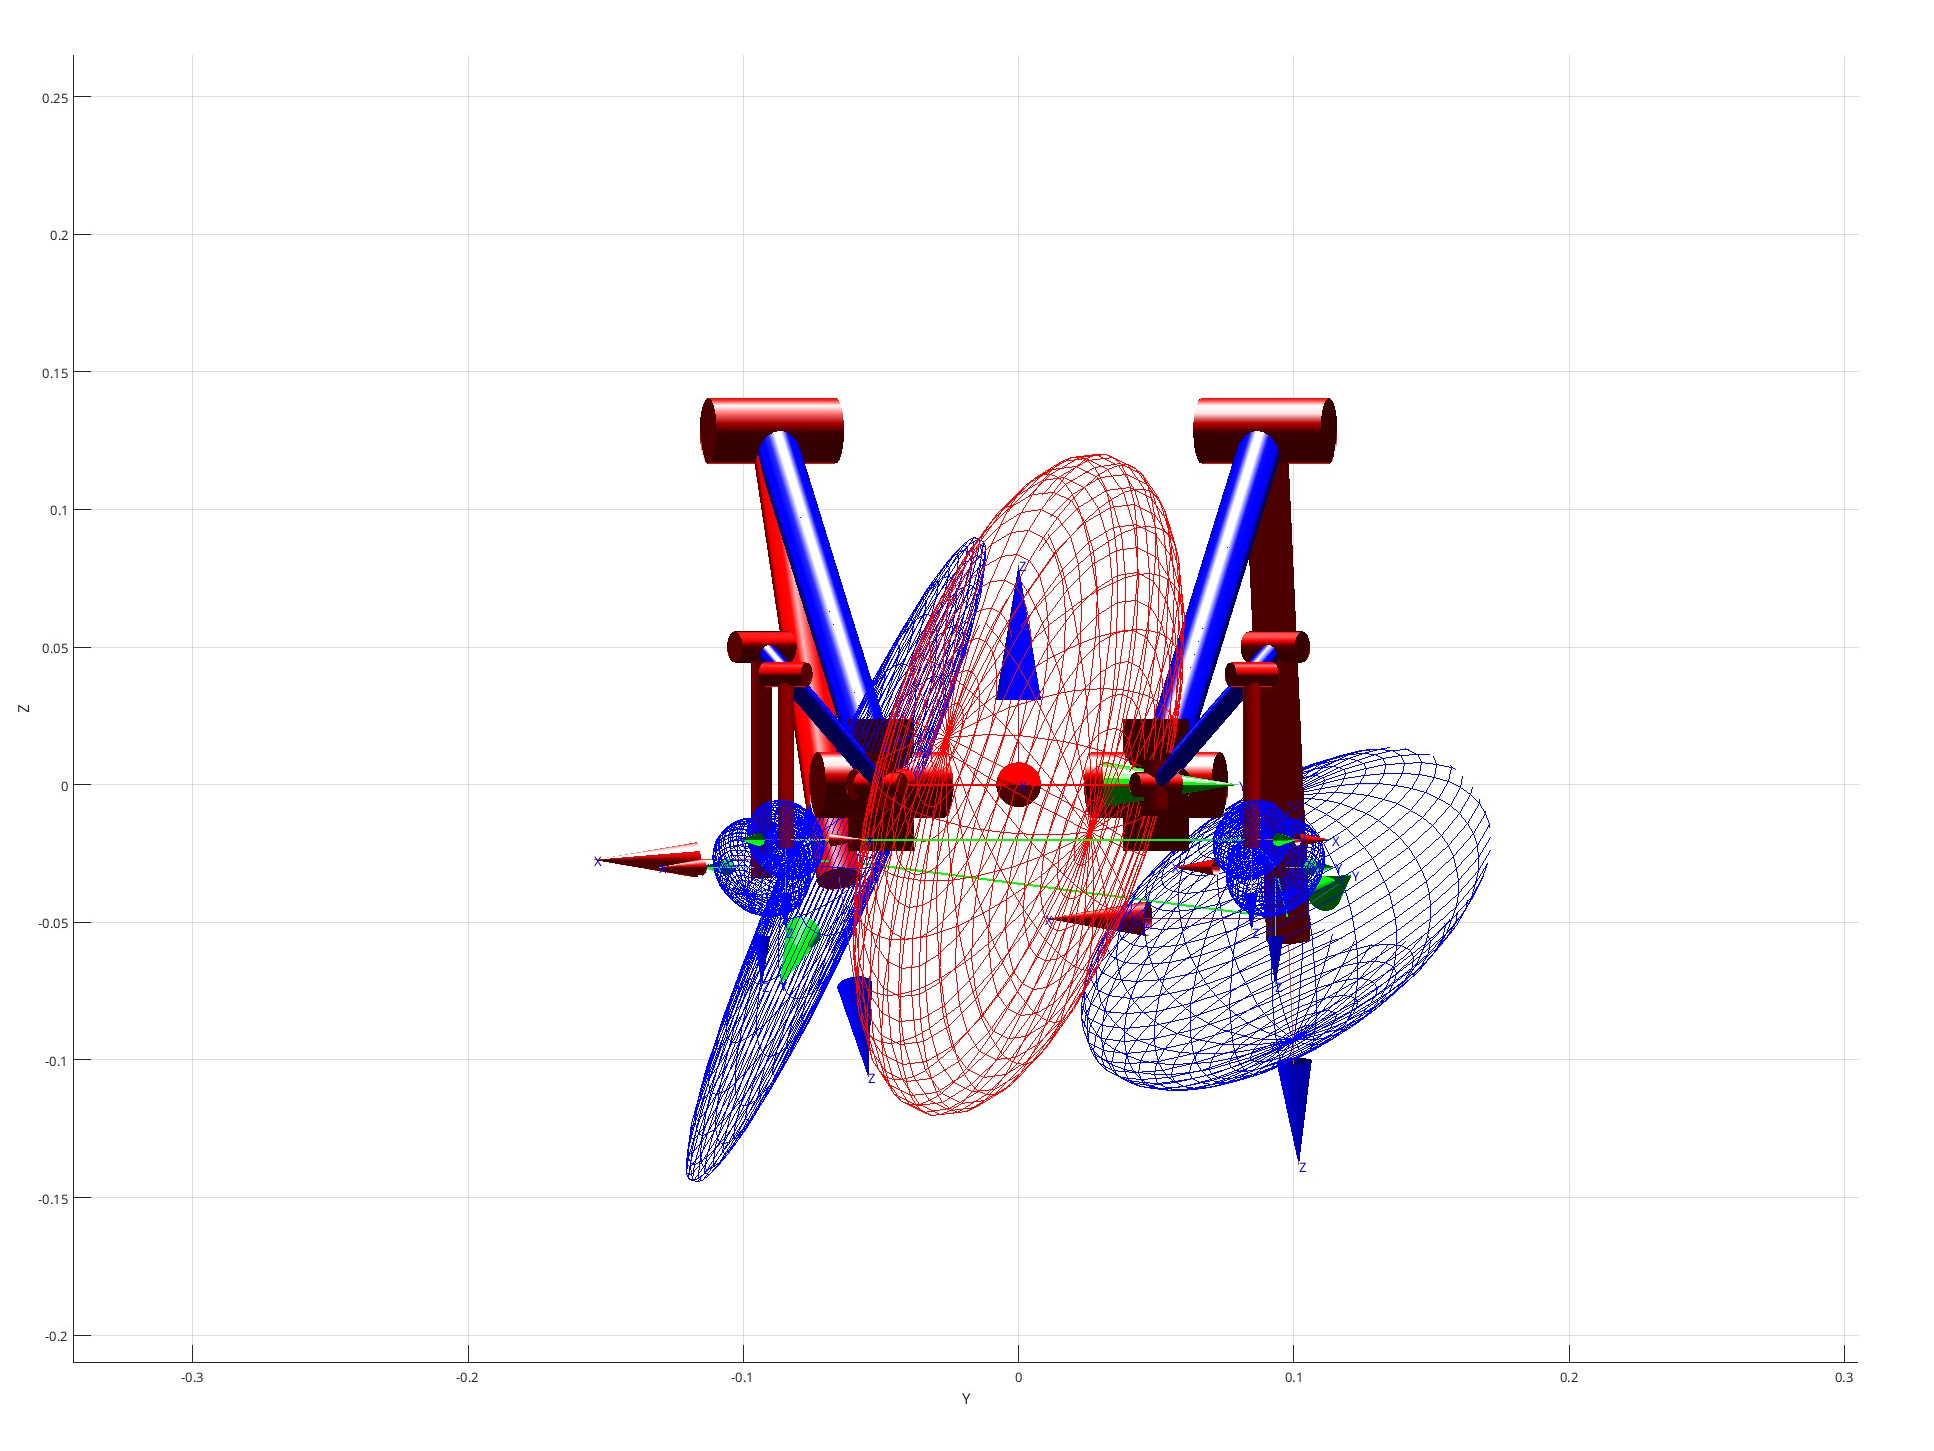
\includegraphics[width=0.5\textwidth]{Images/img_ch3/jumping_Lf2t_120_Rf2t_160_yz.jpg}}\\
    \caption[Asymmetric back legs performances]{Asymmetric back legs performances, with $|B2C| = -15^{\circ}$ and $C2F = -40^{\circ}$.}
    \label{fig:asymmetry}
\end{figure}

\textbf{3) Failure of one back leg}\\
Analyzing possible points of failure is interesting, in this case, to see if the behaviors described by the ellipsoid are coherent. For a robotic system instead, it can provide useful information to define recovery behaviors.  

In the results here, the jumping leg is considered in the configuration:\\ 
$\textbf{q}_{jump,B} = \begin{bmatrix}
    -15^\circ & -40^\circ & 160^\circ
\end{bmatrix}^T$ \\While the other one is irrelevant, since not involved in the motion of the base (removing the ground interaction, represented by the fact that its ellipsoid is green).   

The clear change of maximum direction of the ATBVME in Fig.\ref{fig:one_fail} is coherent with the expected loss of one-leg jumping mobility. 

\begin{figure}[H]
    \centering
    \subfloat[Manipulability without back left leg, top view\label{fig:jumping_NO_BL_xy}]{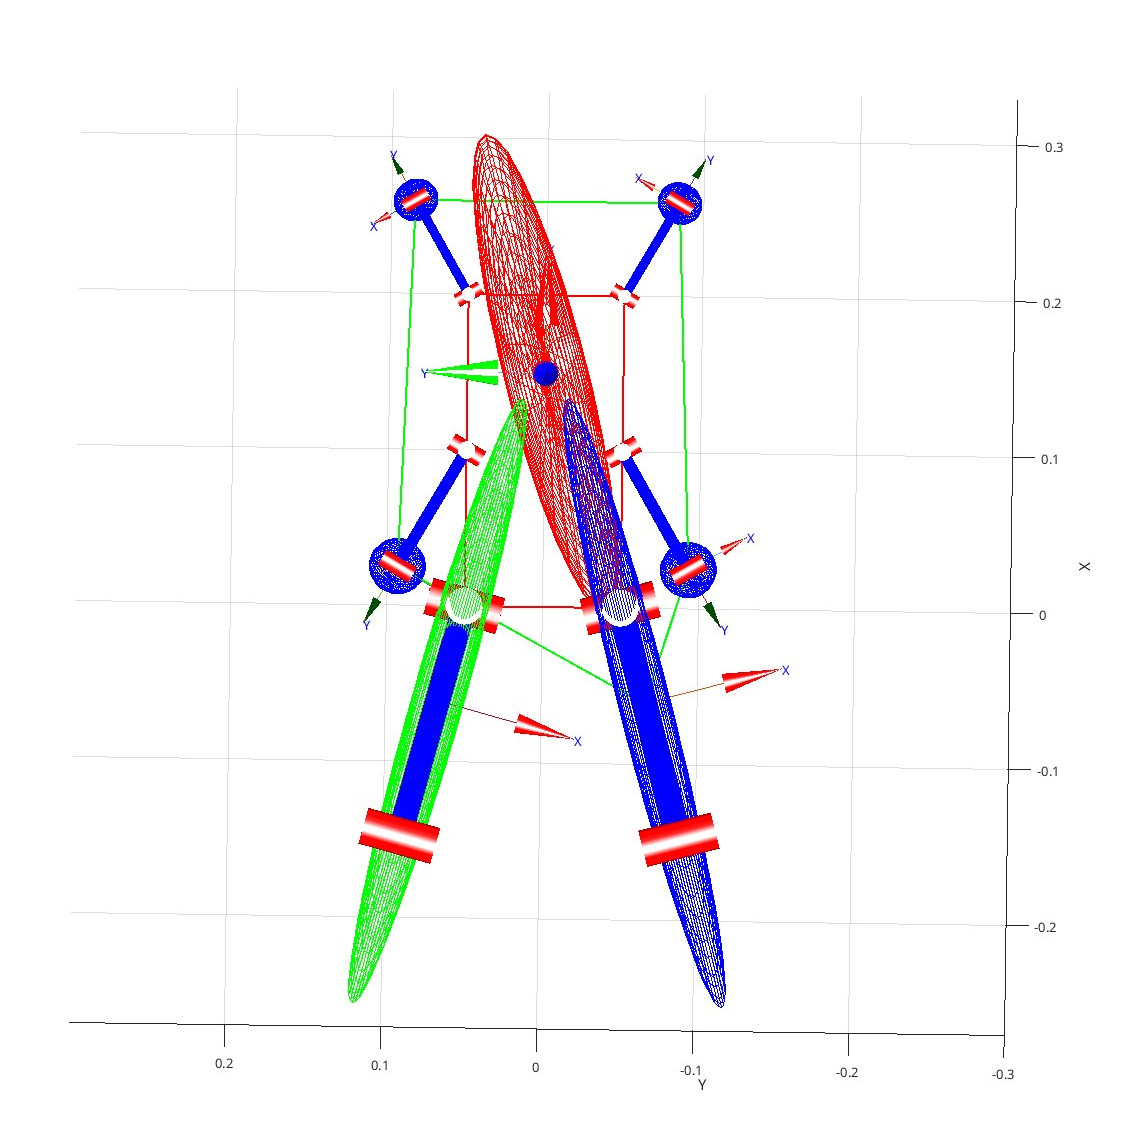
\includegraphics[width=0.5\textwidth]{Images/img_ch3/jumping_NO_BL_xy.jpg}}
    \subfloat[Manipulability without back right leg, top view\label{fig:jumping_NO_BR_xy}]
    {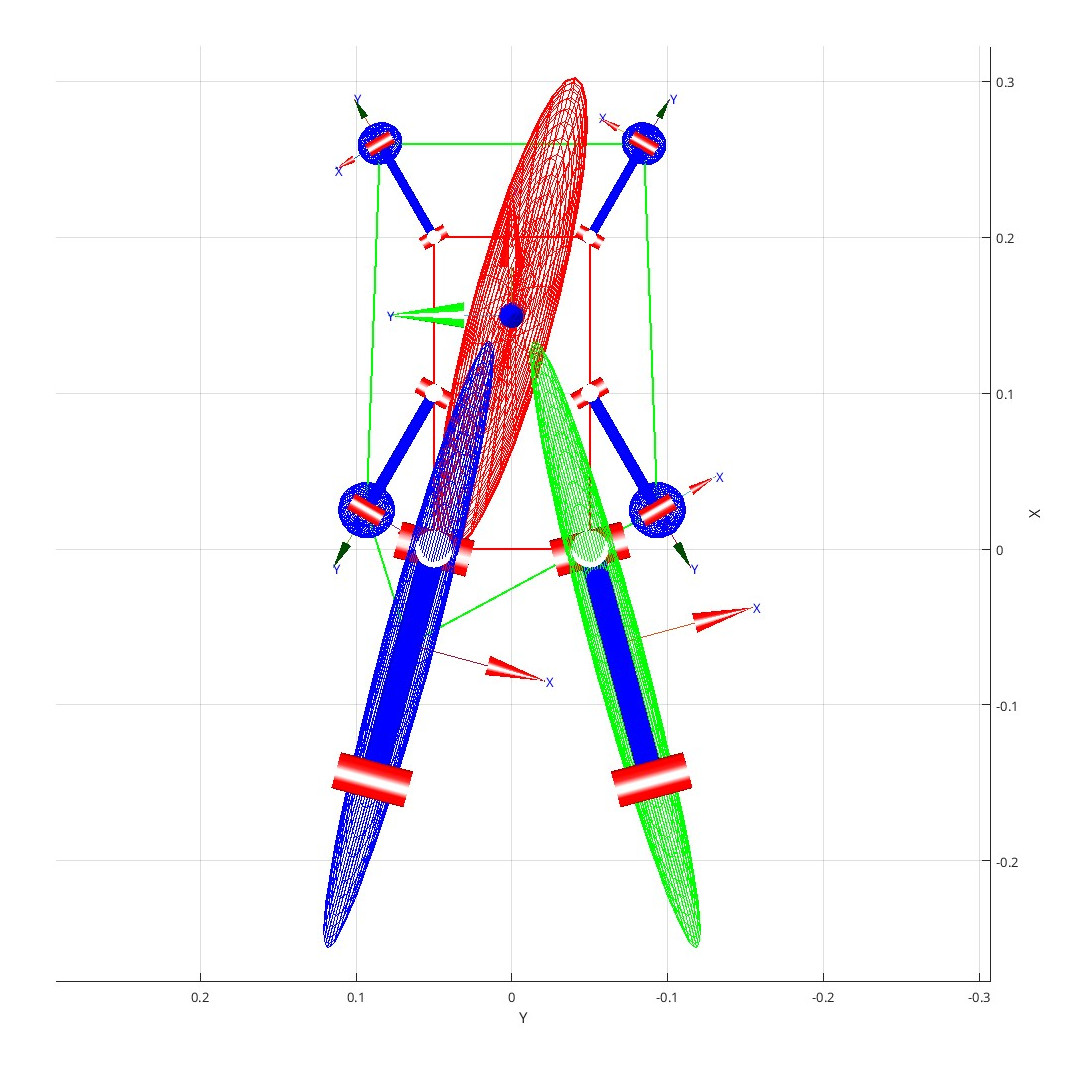
\includegraphics[width=0.5\textwidth]{Images/img_ch3/jumping_NO_BR_xy.jpg}}\\
    \subfloat[Manipulability without back left leg, xz view\label{fig:jumping_NO_BL_xz}]{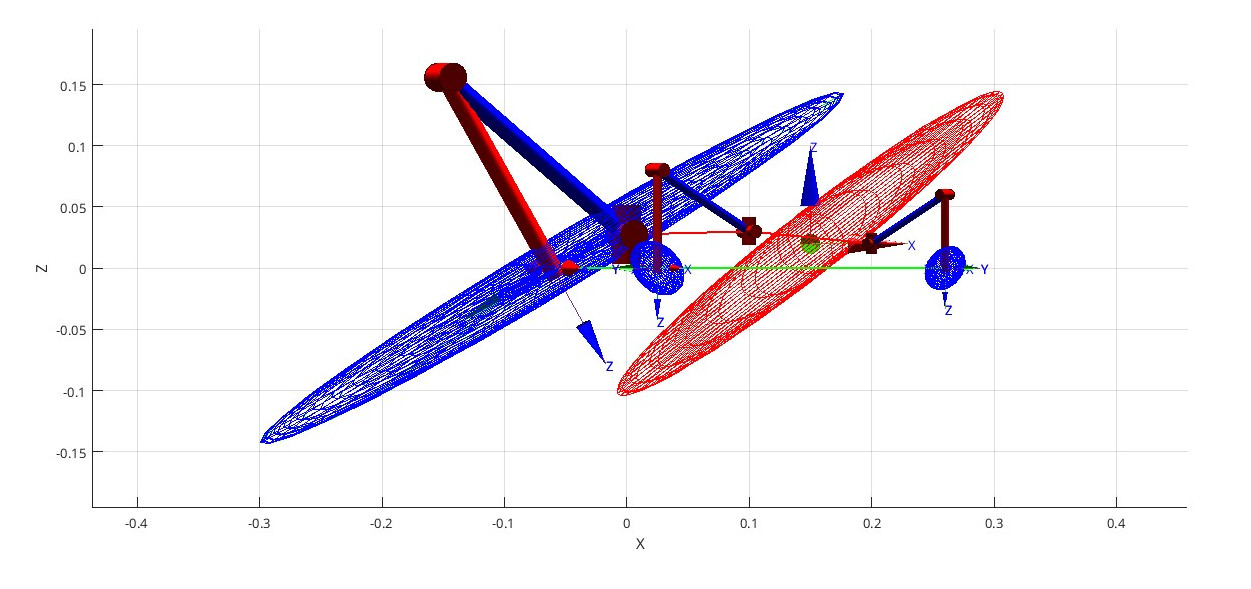
\includegraphics[width=0.5\textwidth]{Images/img_ch3/jumping_NO_BL_xz.jpg}}
    \subfloat[Manipulability without back right leg, xz view\label{fig:jumping_NO_BR_xz}]
    {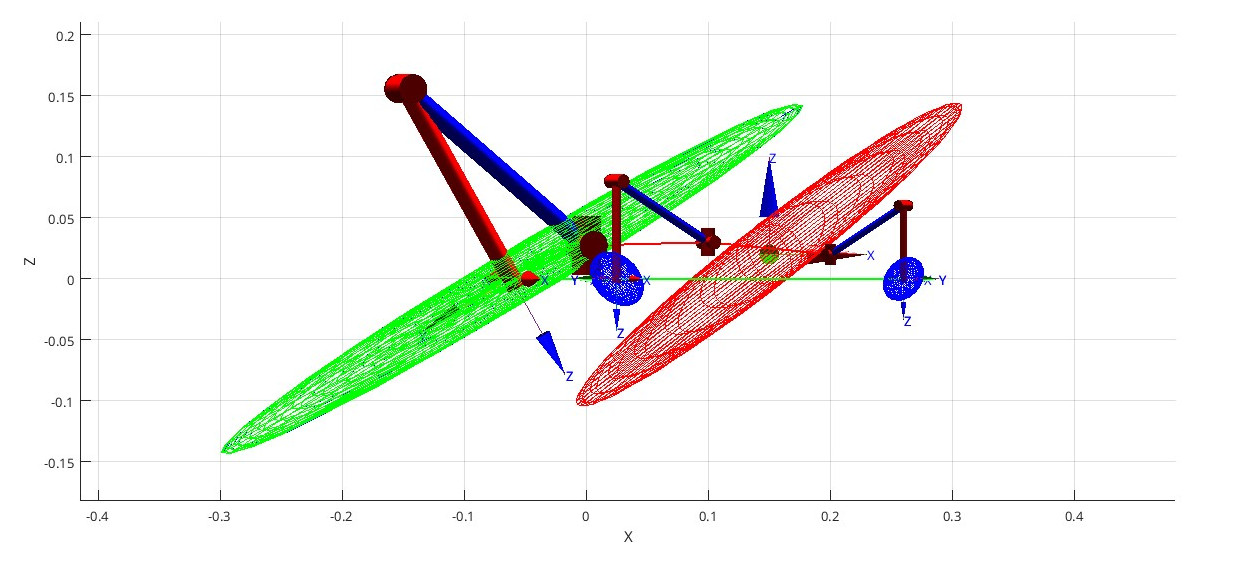
\includegraphics[width=0.5\textwidth]{Images/img_ch3/jumping_NO_BR_xz.jpg}}
    \caption[Jumping performances without one of the back leg]{Jumping performances without one of the back leg.}
    \label{fig:one_fail}
\end{figure}

\textbf{4) Failure of both back legs}\\
Considering a critical failure, in principle it is expected a complete loss of the jumping ability, with only a limited motion capability given by the weak front legs.
The results are reported in Fig.\ref{fig:both_leg_fail}, with a small isotropic ellipsoid, without any dominating jumping axis. 

\begin{figure}[H]
    \centering
    \subfloat[Manipulability without jumping legs, xy view\label{fig:jumping_NO_B_xy}]{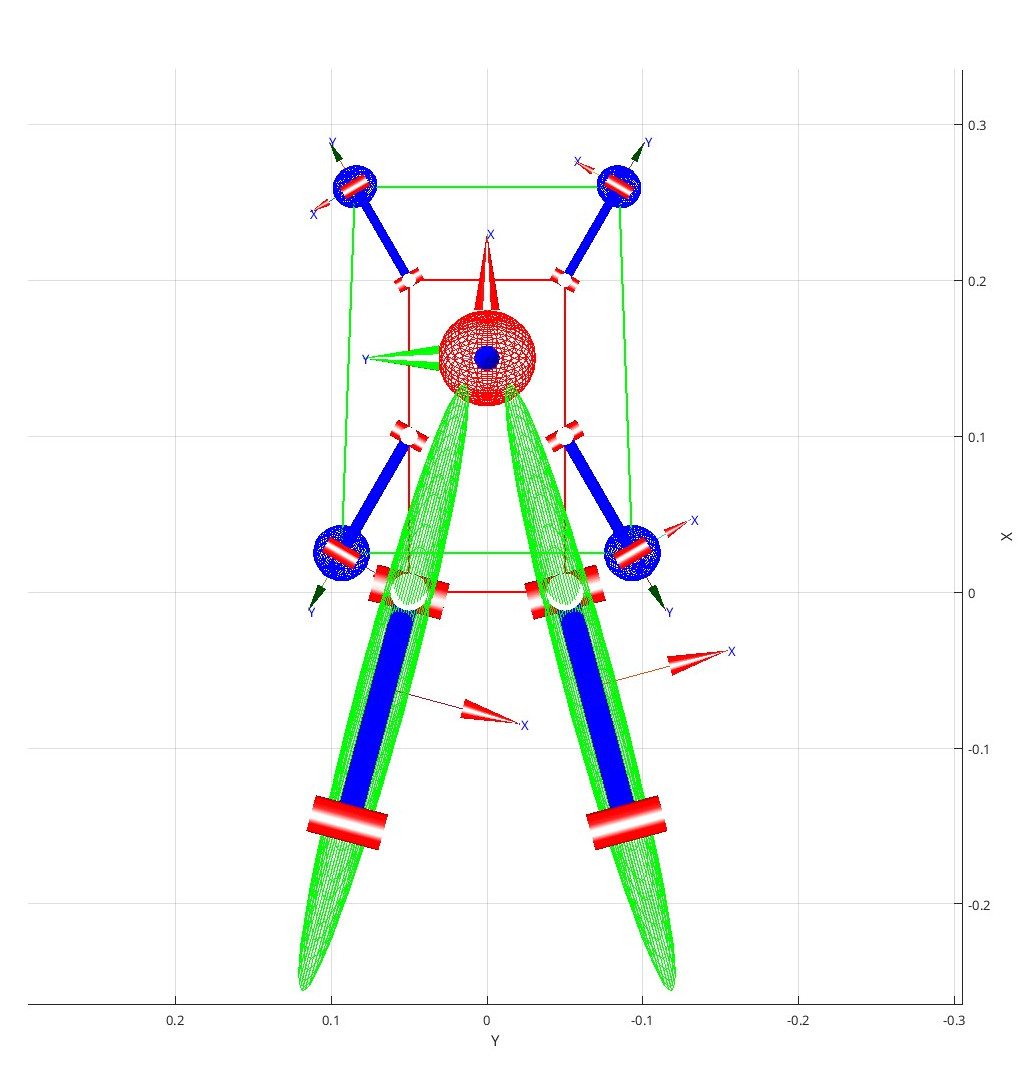
\includegraphics[width=0.5\textwidth]{Images/img_ch3/jumping_NO_B_xy.jpg}}
    \subfloat[Manipulability without jumping legs, xz view\label{fig:jumping_NO_B_xz}]
    {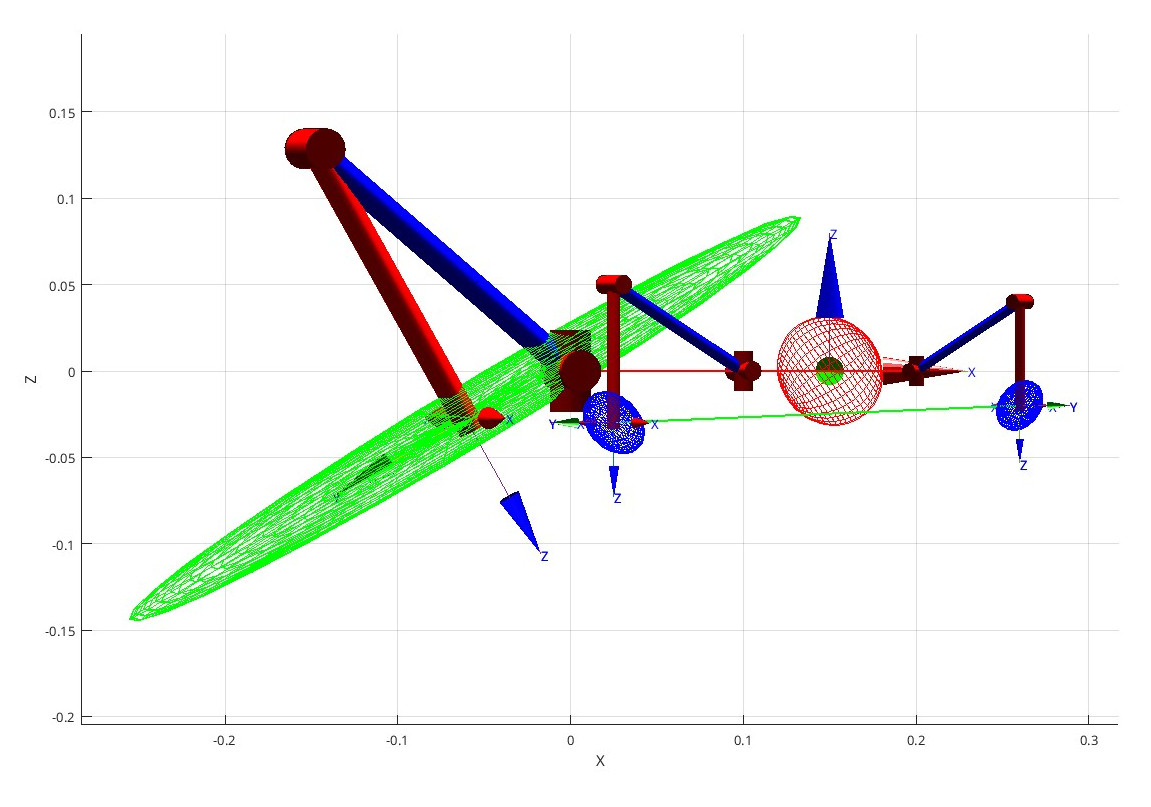
\includegraphics[width=0.5\textwidth]{Images/img_ch3/jumping_NO_B_xz.jpg}}
    \caption[Manipulability without jumping legs]{Manipulability without jumping legs}
    \label{fig:both_leg_fail}
\end{figure}

\textbf{5) CoM position, Sensitivity Analysis}\\
What happens to the manipulability ellipsoid when the CoM position changes is an interesting question. 
This is especially relevant for systems that can 
lose/gain parts or change its structure depending on the task.
Again the back legs are considered in 
$\mathbf{q}_{LB} =\mathbf{q}_{RB} = \begin{bmatrix}
    -15^\circ & -40^\circ & 160^\circ
\end{bmatrix}^T$\\
As reported in Fig.\ref{fig:CoM_changes}, the CoM is translated in the midpoint between the two back legs.
\begin{figure}[H]
    \centering
    \subfloat[xy view\label{fig:jumping_CoM_0_xy}]
    {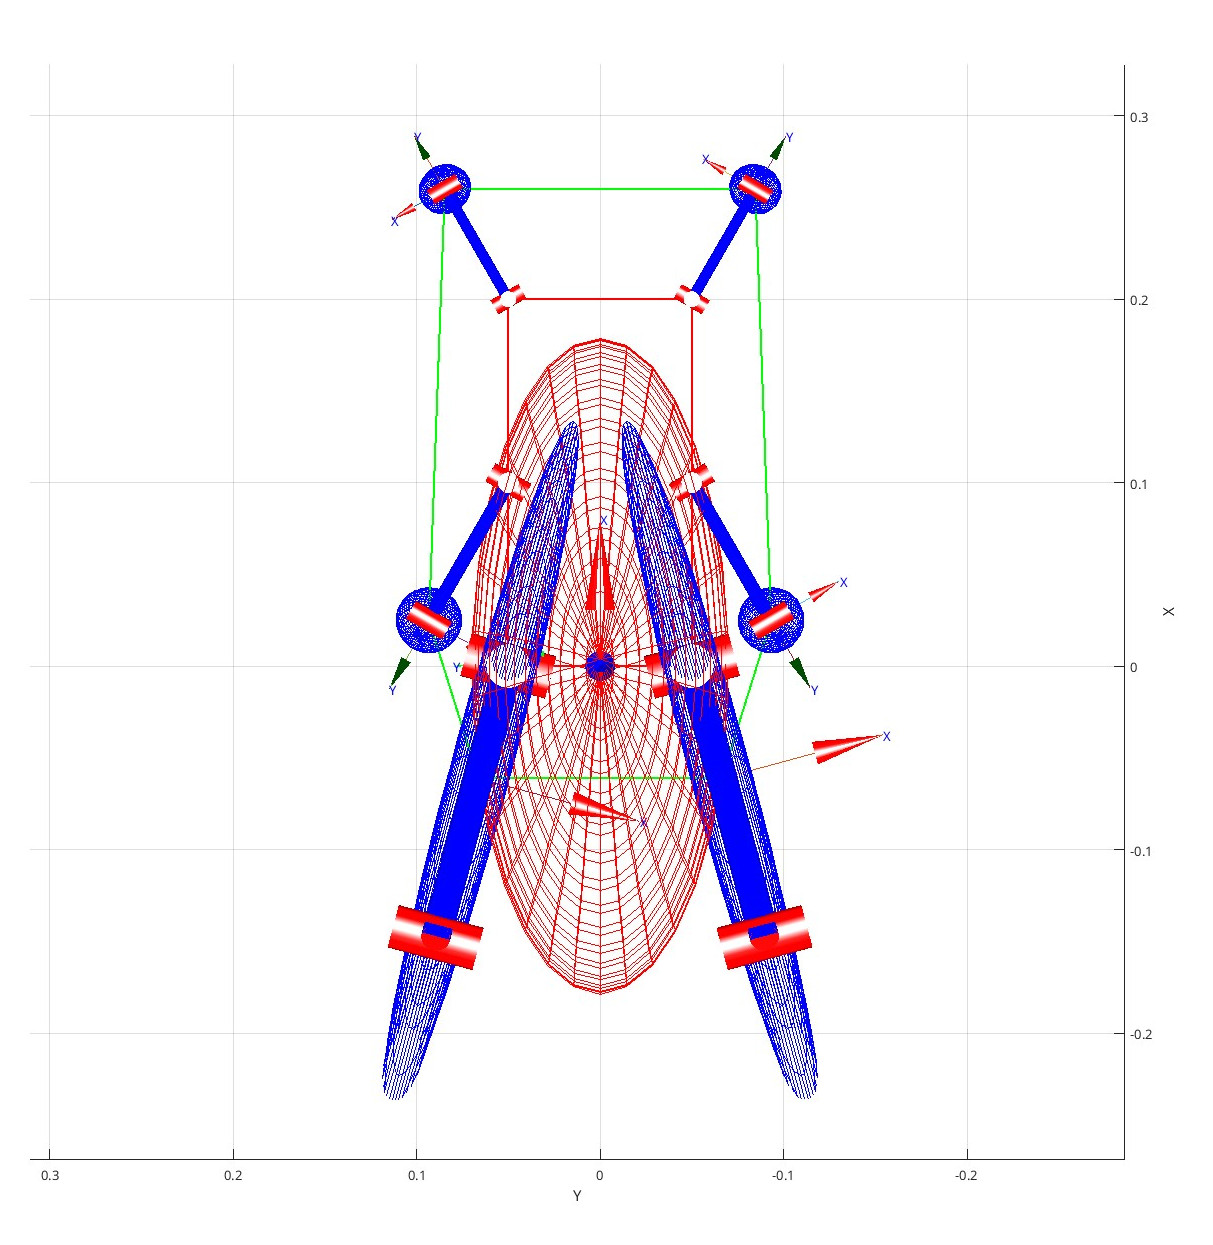
\includegraphics[width=0.4\textwidth]{Images/img_ch3/jumping_CoM_0_xy.jpg}}
    \subfloat[xz view\label{fig:jumping_CoM_0_xy}]
    {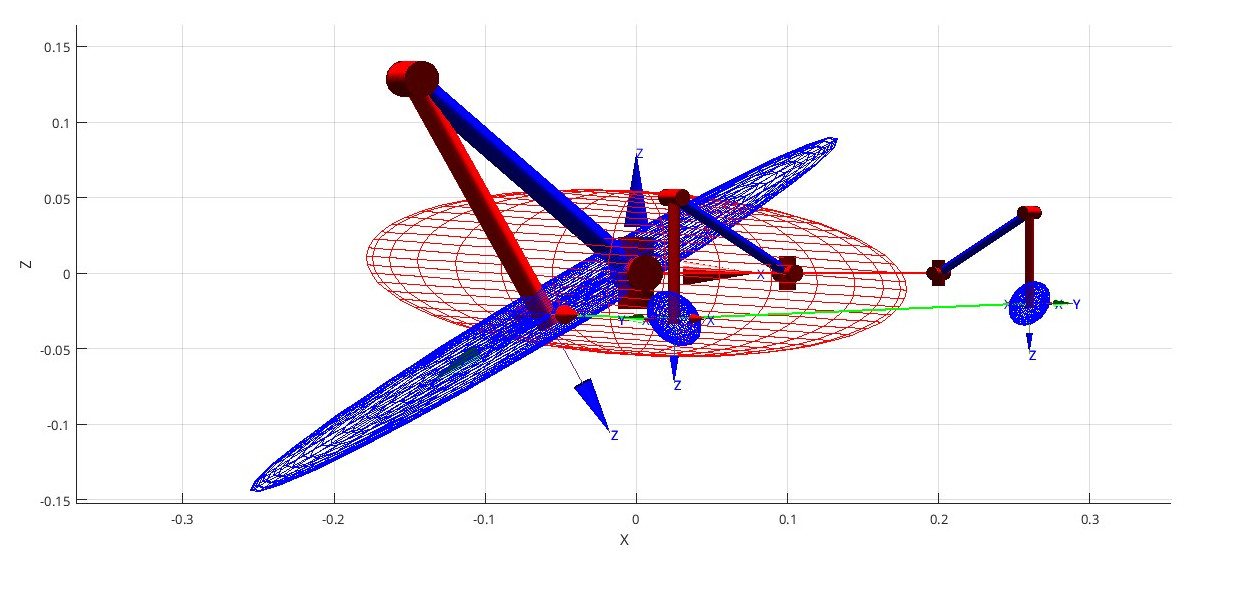
\includegraphics[width=0.4\textwidth]{Images/img_ch3/jumping_CoM_0_xz.jpg}}
    \caption[Jumping with different CoM]{Jumping with the CoM in the midpoint of the back legs}
    \label{fig:CoM_changes}
\end{figure}


\subsection{Final Comments on Multi-Limb robot base ME}
\label{sec:Conclusions}

The results of the examples above prove that the ATBVME is an intuitive and powerful geometrical tool, to identify the preferred direction of base motion. The ellipsoids obtained in all the configurations are consistent with the one expected by an extension of the original theory. Unfortunately, some of the limitations of the manipulability theory are reflected here, and in some cases, even if the shape is correct, the dimensions are just indicative and possibly misleading. 

For this reason, in the current formulation, this theory is useful to estimate directions with good mobility, but not accurate for defining quantitative indices to optimize. 
The scaling approach used for the grasshopper example has been tested also in LimbedEx1 and LimbedEx2, obtaining more meaningful ellipsoid axis ratios, but still high volume in inefficient configurations. 

Nevertheless, this approach is useful for multi-limbed robots with complex limb designs, characterized by unexpected possible base motion, identifiable using the major axis of the ATBVME. For this reason, it will be used to analyze the mobility of the robotic system used in this research and introduced in the following chapter, LIMBERO-GRIEEL.


